%
% $Id:  ENTER YOUR ID/FILENAME HERE$
%
% This template is based on LLNCS.DEM, the demonstration file of the LaTeX macro 
% package from Springer-Verlag for Lecture Notes in Computer Science, version 2.2 for
% LaTeX2e (see llncs.dem for usage information).
% The template uses the additional definitions based on the master-thesis of Alexander 
% Holupirek (University of Konstanz) and Thomas Zink (University of Konstanz).
% 
% This template was adapted and generalized by Sebastian Kay Belle (University of
% Konstanz) as a generic template for bachelor and master theses (at least for the
% students of the distributed systems laboratory).
%
% Sebastian Kay Belle -- Distributed Systems Laboratory
% Department of Computer and Information Science -- University of Konstanz
% 


% one-sided document style suited for bachelor/master theses (english)
\documentclass[a4paper]{llncs} 
% two-sided document sytel suited for bachelor/master theses (english)
%\documentclass[twoside,a4paper]{llncs} 
% one-sided document sytel suited for bachelor/master theses (german)
%\documentclass[ngerman,a4paper]{llncs} 
% two-sided document sytel suited for bachelor/master theses (german)
%\documentclass[ngerman,twoside,a4paper]{llncs} 

%%%%%%%%%%%%%%%%%%%%%%%%%%%%%%%%%%%%%%%%%%%%%%%%%%%%%%%%%%%%%%%%%%%%%%%%%%%%%%%%%%%%%%%%%%%%%%%%%%%%%%%%%%%%%%%%%
%%% PACKAGES
%%%%%%%%%%%%%%%%%%%%%%%%%%%%%%%%%%%%%%%%%%%%%%%%%%%%%%%%%%%%%%%%%%%%%%%%%%%%%%%%%%%%%%%%%%%%%%%%%%%%%%%%%%%%%%%%%
%\usepackage{tocbibind}
\usepackage{graphicx}			% graphics, of course
\usepackage{color}                      % to define colors
\usepackage{amsmath, amssymb}		% math symbols for sets etc
\usepackage{multirow}			% for table and tabular, allows multirows and cols
\usepackage[linesnumbered,ruled,vlined,commentsnumbered]{algorithm2e} % extended algorithm package
%\usepackage{ulem}			% for underlining, also changes \em to \underline
					% use \mormalem to undo, however,
					% somehow removes references from toc
\usepackage{fancyvrb}			% fancy verbatim
\usepackage{fancyhdr}                  	% fancy header
\usepackage[colorinlistoftodos]{todonotes} % todo notes
\usepackage{listings}
\usepackage{hyperref}			% hypertext references, somehow screws up with figures
\usepackage[all]{hypcap}
%\usepackage[svgnames]{xcolor}

%%%%%%%%%%%%%%%%%%%%%%%%%%%%%%%%%%%%%%%%%%%%%%%%%%%%%%%%%%%%%%%%%%%%%%%%%%%%%%%%%%%%%%%%%%%%%%%%%%%%%%%%%%%%%%%%%
%%% SETTINGS
%%%%%%%%%%%%%%%%%%%%%%%%%%%%%%%%%%%%%%%%%%%%%%%%%%%%%%%%%%%%%%%%%%%%%%%%%%%%%%%%%%%%%%%%%%%%%%%%%%%%%%%%%%%%%%%%%
\graphicspath{figures/}			% somehow, doesn't work, thus use command
%\newcommand{\gfx}[0]{../gfx/}
\titlerunning{~}				% set off for llncs	
\authorrunning{~}				% set off for llncs

\newtheorem{thm}{Lemma}%[]             % lemma definition
\newcommand{\factor}[0]{10}

% Listing of algorithms (bug in algorithm2e)
%\renewcommand{\listofalgorithms}{\tocfile{\listalgorithmcfname}{loa}} 

% Bullets for list items
\renewcommand{\labelitemi}{$\bullet$}

% Listings
\lstset{numbers=left, numberstyle=\tiny, stepnumber=1, numbersep=5pt, language=xml, basicstyle=\footnotesize,
 keywordstyle=\color{blue!80!black!100},}

%%%%%%%%%%%%%%%%%%%%%%%%%%%%%%%%%%%%%%%%%%%%%%%%%%%%%%%%%%%%%%%%%%%%%%%%%%%%%%%%%%%%%%%%%%%%%%%%%%%%%%%%%%%%%%%%%
%%% SETTINGS FOR THE HYPERREF PACKAGE
%%%%%%%%%%%%%%%%%%%%%%%%%%%%%%%%%%%%%%%%%%%%%%%%%%%%%%%%%%%%%%%%%%%%%%%%%%%%%%%%%%%%%%%%%%%%%%%%%%%%%%%%%%%%%%%%%
\definecolor{internal-link}{rgb}{0.2, 0.26, 0.43}
\definecolor{cite-link}{rgb}{0.4, 0.61, 0.46}
\definecolor{url-link}{rgb}{0.4, 0.46, 0.63}

\hypersetup{
  colorlinks=true,
  linkcolor=internal-link,
  citecolor=cite-link,
  urlcolor=url-link
}

%%%%%%%%%%%%%%%%%%%%%%%%%%%%%%%%%%%%%%%%%%%%%%%%%%%%%%%%%%%%%%%%%%%%%%%%%%%%%%%%%%%%%%%%%%%%%%%%%%%%%%%%%%%%%%%%%
%%% KW SETTINGS FOR ALGORITHMS2E (see algorithm2e documentation for details)
%%%%%%%%%%%%%%%%%%%%%%%%%%%%%%%%%%%%%%%%%%%%%%%%%%%%%%%%%%%%%%%%%%%%%%%%%%%%%%%%%%%%%%%%%%%%%%%%%%%%%%%%%%%%%%%%%
% define your language keywords here (e.g. \SetKw{To}{to})
%\SetKw{To}{to}
%\SetKw{Not}{not}
% define your data keywords here (e.g. \SetKwData{Counters}{counters})
% define your function keywords here (e.g. \SetKwFunction{Compress}{Compress})

%%%%%%%%%%%%%%%%%%%%%%%%%%%%%%%%%%%%%%%%%%%%%%%%%%%%%%%%%%%%%%%%%%%%%%%%%%%%%%%%%%%%%%%%%%%%%%%%%%%%%%%%%%%%%%%%%
%%% HEADER/FOOTER (see the fancyhdr documentation for details)
%%%%%%%%%%%%%%%%%%%%%%%%%%%%%%%%%%%%%%%%%%%%%%%%%%%%%%%%%%%%%%%%%%%%%%%%%%%%%%%%%%%%%%%%%%%%%%%%%%%%%%%%%%%%%%%%%
\setlength{\headheight}{15pt}
 
\pagestyle{fancy}
\renewcommand{\chaptermark}[1]{\markboth{#1}{}}
\renewcommand{\sectionmark}[1]{\markright{#1}{}}
\renewcommand{\headrulewidth}{0.5pt}
\renewcommand{\footrulewidth}{0.5pt}
 
\fancyhf{}
\fancyhead[LE,RO]{\thepage}
\fancyhead[RE,LO]{\textit{\nouppercase{\rightmark}}}
\fancyfoot[EL,OR]{\thepage}
 
\fancypagestyle{plain}{ %
\fancyhf{} % remove everything
\renewcommand{\headrulewidth}{0pt} % remove lines as well
\renewcommand{\footrulewidth}{0pt}}

%%%%%%%%%%%%%%%%%%%%%%%%%%%%%%%%%%%%%%%%%%%%%%%%%%%%%%%%%%%%%%%%%%%%%%%%%%%%%%%%%%%%%%%%%%%%%%%%%%%%%%%%%%%%%%%%%
%%% OTHER DEFINITIONS
%%%%%%%%%%%%%%%%%%%%%%%%%%%%%%%%%%%%%%%%%%%%%%%%%%%%%%%%%%%%%%%%%%%%%%%%%%%%%%%%%%%%%%%%%%%%%%%%%%%%%%%%%%%%%%%%%
\def\dotuline{\bgroup
  \ifdim\ULdepth=\maxdimen  % Set depth based on font, if not set already
   \settodepth\ULdepth{(j}\advance\ULdepth.4pt\fi
  \markoverwith{\begingroup
  \advance\ULdepth0.08ex
  \lower\ULdepth\hbox{\kern.15em .\kern.1em}%
  \endgroup}\ULon}

\def\dashuline{\bgroup
  \ifdim\ULdepth=\maxdimen  % Set depth based on font, if not set already
   \settodepth\ULdepth{(j}\advance\ULdepth.4pt\fi
  \markoverwith{\kern.15em
  \vtop{\kern\ULdepth \hrule width .3em}%
  \kern.15em}\ULon}

% --- verbatim environments
%\VerbatimFootnotes 
\DefineVerbatimEnvironment{xml}{Verbatim}
{
% gobble=2,
  frame=single,% framerule=0.25pt,
% xleftmargin=1em, xrightmargin=1em,
  fontfamily=courier, fontsize=\scriptsize,
  commandchars=\\\{\}
}
\DefineVerbatimEnvironment{fs}{Verbatim}
{
% gobble=2,
  frame=lines, framesep=3mm,
  labelposition=topline,
  fontfamily=courier, fontsize=\footnotesize,
  commandchars=\\\{\}
}
\DefineVerbatimEnvironment{xquery}{Verbatim}
{
% gobble=2,
  frame=lines, framesep=3mm,
  labelposition=topline,
  %framerule=0.4pt, % default 0.4pt
  fontfamily=courier, fontsize=\footnotesize,
  commandchars=\\\{\}
}

% Definition environment
\newtheorem{mydef}{Definition}

%%%%%%%%%%%%%%%%%%%%%%%%%%%%%%%%%%%%%%%%%%%%%%%%%%%%%%%%%%%%%%%%%%%%%%%%%%%%%%%%%%%%%%%%%%%%%%%%%%%%%%%%%%%%%%%%%
%%% DOCUMENT
%%%%%%%%%%%%%%%%%%%%%%%%%%%%%%%%%%%%%%%%%%%%%%%%%%%%%%%%%%%%%%%%%%%%%%%%%%%%%%%%%%%%%%%%%%%%%%%%%%%%%%%%%%%%%%%%%
\begin{document}

%%%%%%%%%%%%%%%%%%%%%%%%%%%%%%%%%%%%%%%%%%%%%%%%%%%%%%%%%%%%%%%%%%%%%%%%%%%%%%%%%%%%%%%%%%%%%%%%%%%%%%%%%%%%%%%%%
%%% TITLE PAGE -- CHOOSE THE APPROPRIATE TITLE PAGE HERE (AND MODIFY THEM TO YOUR LIKING)
%%%%%%%%%%%%%%%%%%%%%%%%%%%%%%%%%%%%%%%%%%%%%%%%%%%%%%%%%%%%%%%%%%%%%%%%%%%%%%%%%%%%%%%%%%%%%%%%%%%%%%%%%%%%%%%%%
\pagenumbering{alph}
\pagestyle{empty}
%\pagestyle{plain}
%\input{titlepage_std_en} % include your titlepage here (standard title page)
%\input{titlepage_std-signet_en} % include your titlepage here (standard title page with university signet)
\begin{titlepage}
\begin{minipage}{0.9\linewidth}
\end{minipage}
\vfill
%\begin{center}
%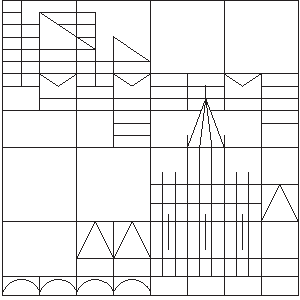
\includegraphics[scale=1]{figures/signet} % signet U KN
%\end{center}
%\vspace{10mm}
%\vfill
{\sf
\begin{center}
{\Large University of Konstanz} \\
\vspace{2mm}{\Large Department of Computer and Information Science} \\ 
\vspace{4mm}
\rule{0.98\linewidth}{2pt}\\
\vspace{4mm} 
{\huge {\bf {\sffamily{Master Thesis}}}}\\
\vspace{10mm}
{\huge A Visual Analytics Approach for Comparing Tree-Structures.}\\
\vspace{10mm}
{\em {\sffamily{in fulfillment of the requirements to achieve the degree of \\ 
\vspace{2mm} {\bf \sffamily{Master of Science (M.Sc.)}}}}}\\
\vspace{2mm}
\rule{0.98\linewidth}{2pt}\\
\vspace{6mm}{\Large \bf \sffamily{Johannes Lichtenberger}}\\
\vspace{0mm}{Matriculation Number :: 01/584875}\\
\vspace{0mm}{E-Mail :: $\langle$firstname$\rangle$.$\langle$lastname$\rangle$@uni-konstanz.de}\\
\vspace{6mm}
{\small
\begin{tabular}{l  p{5mm}  r}
{\bf {\sffamily{Field of Study}}} ::  Information Engineering & & {\bf \sffamily{First Assessor}} ::  {\em Prof. Dr. M. Waldvogel}\\
{\bf {\sffamily{Focus}}} :: {\em } & & {\bf \sffamily{Second Assessor}} ::  {\em Jun.-Prof. Dr. Tobias Schreck}\\
{\bf {\sffamily{Topic}}} :: {\em } & & {\bf \sffamily{Advisor}} ::  {\em M.Sc. Sebastian Graf}\\
\end{tabular}\\
}
\end{center}
}
\vfill
\end{titlepage}




 % include your titlepage here (unconventional title page with university signet above 
%\input{titlepage_fancy-teaser_en} % include your titlepage here (unconventional title page with space for a teaser image)
%\pagestyle{fancy}

%%%%%%%%%%%%%%%%%%%%%%%%%%%%%%%%%%%%%%%%%%%%%%%%%%%%%%%%%%%%%%%%%%%%%%%%%%%%%%%%%%%%%%%%%%%%%%%%%%%%%%%%%%%%%%%%%
%%% PREAMBLE
%%%%%%%%%%%%%%%%%%%%%%%%%%%%%%%%%%%%%%%%%%%%%%%%%%%%%%%%%%%%%%%%%%%%%%%%%%%%%%%%%%%%%%%%%%%%%%%%%%%%%%%%%%%%%%%%%
\newpage
\pagestyle{fancy}
\voffset=10mm % optical enhancement!!!
\pagenumbering{roman} % set the page numbering style to roman numbers
\cleardoublepage
\thispagestyle{empty}
\vspace*{0.5\textheight}
\begin{center}
dedicated to...
\end{center}
\newpage
 % refer your preamble here

%%%%%%%%%%%%%%%%%%%%%%%%%%%%%%%%%%%%%%%%%%%%%%%%%%%%%%%%%%%%%%%%%%%%%%%%%%%%%%%%%%%%%%%%%%%%%%%%%%%%%%%%%%%%%%%%%
%%% ABSTRACT
%%%%%%%%%%%%%%%%%%%%%%%%%%%%%%%%%%%%%%%%%%%%%%%%%%%%%%%%%%%%%%%%%%%%%%%%%%%%%%%%%%%%%%%%%%%%%%%%%%%%%%%%%%%%%%%%%
\newpage
\setcounter{page}{1}
\begin{abstract}
Todays storage capabilities facilitate the accessibility and long term archival of increasingly large data sets usually refered to as "Big Data". Tree-structured hierarchical data is very common, for instance phylogenetic trees, filesystem data, syntax trees and often times organizational structures. Analysts often face the problem of gathering information through comparison of multiple trees. However large amounts of data lead to an information overload. Visual analytic tools aid analysts by combining visual clues and analytical reasoning. Visual representations are ideal as they tend to stress human strength which are great at interpreting visualizations.

We therefore propose a prototype for comparing tree-structures which either evolve through time or usually share large node-sets. Our backend Treetank is a tree-storage system designed to persist several revisions of a tree-structure efficiently. Differend types of similarity measures are implemented adhering to the well known tree-to-tree edit problem. The Fast Matching Simple Editscript-algorithm published in a paper by Chawathe is implemented to support the comparison of ID-less trees and to store these differences as a new revision in Treetank. Based on unique stable node-IDs through time we are able to use a novel ID-based diff-algorithm to build an aggregated tree-structure formed by comparing different revisions.

The aggregated tree-structure is input to several interactive visualizations. A novel Sunburst-layout facilitates the comparison between two revisions and besides providing several other visualization options supports zooming as well as drilling down into the tree by selecting a new root node. Besides inserted, deleted and updated nodes moved- and replaced-nodes are optionally depicted to improve expressiveness. Hierarchical edge bundles are used to visualize moves. Furthermore several filtering-techniques are available to compare even very large tree-structures up to many hundred thousand or even millions of nodes. Small multiple variants of the Sunburst-layout aid the comparison between multiple trees. A text view furthermore depicts a serialization of the aggregated tree-structure in form of syntax highlighted XML. To support large trees only visible content is serialized plus an additional overhead to support scrolling which appends lines on demand. The views are synchronized.

A short evaluation based on a few criterias and a study of three application scenarios as well as performance evaluations proves the applicability of our approach. In comparison to other approaches to the best of our knowledge besides TreeJuxtaposer our approach is the only one which facilitates the comparison of large trees. Furthermore we support the comparsion of generic rooted, labeled trees whereas other approaches are specifically designed for certain domains and often times either the comparison is based on IDs or the algorithm is not usable for other domains. Thus our approach clearly surpasses most other approaches in terms of generability and scalability due to our database driven approach which allows for a fast ID-based difference algorithm optionally using hashes for filtering changed subtrees.
\end{abstract}
 % refer your abstract here
\addcontentsline{toc}{section}{\abstractname}

%%%%%%%%%%%%%%%%%%%%%%%%%%%%%%%%%%%%%%%%%%%%%%%%%%%%%%%%%%%%%%%%%%%%%%%%%%%%%%%%%%%%%%%%%%%%%%%%%%%%%%%%%%%%%%%%%
%%% TABLE OF CONTENT, LIST OF FIGURES & LIST OF TABLES
%%%%%%%%%%%%%%%%%%%%%%%%%%%%%%%%%%%%%%%%%%%%%%%%%%%%%%%%%%%%%%%%%%%%%%%%%%%%%%%%%%%%%%%%%%%%%%%%%%%%%%%%%%%%%%%%%
\newpage
\pagestyle{fancy}
\setcounter{tocdepth}{2}
\tableofcontents
\newpage
\pagestyle{fancy}
\addcontentsline{toc}{section}{\listfigurename}
\listoffigures
\newpage
\pagestyle{fancy}
\addcontentsline{toc}{section}{\listalgorithmcfname}
\listofalgorithms
\newpage
\pagestyle{fancy}
\addcontentsline{toc}{section}{\lstlistlistingname}
\lstlistoflistings
\newpage
\pagestyle{fancy}
\addcontentsline{toc}{section}{\listtablename}
\listoftables
\newpage
\listoftodos
%\addcontentsline{toc}{section}{\listtodoname}

%%%%%%%%%%%%%%%%%%%%%%%%%%%%%%%%%%%%%%%%%%%%%%%%%%%%%%%%%%%%%%%%%%%%%%%%%%%%%%%%%%%%%%%%%%%%%%%%%%%%%%%%%%%%%%%%%
%%% SECTIONS
%%%%%%%%%%%%%%%%%%%%%%%%%%%%%%%%%%%%%%%%%%%%%%%%%%%%%%%%%%%%%%%%%%%%%%%%%%%%%%%%%%%%%%%%%%%%%%%%%%%%%%%%%%%%%%%%%
\cleardoublepage
\pagestyle{fancy}
\pagenumbering{arabic} % set the page numbering to arabic page numbers
\setcounter{page}{1}
\section{Introduction}\label{sec::introduction}
\subsection{Motivation}
% Overall context
Ever growing amounts of data require effective and efficient storage solutions as well as highly scalable, interactive methods to gain new insights through exploratory analysis or to prove assumptions. Almost all data is subject to change. Nowadays storage is cheap and adheres to Moore's law\cite{MOORE} of doubling about every 18 months supporting the storage of several snapshots of time varying data. Furthermore existing storage techniques minimize the impact of storing such potentially very large data-sets.

Hierarichal information in the form of tree-structures is inherent to many datasets. It is almost always mapped through primary-/foreign-key relations in relational databases. Whereas this might be sufficient in many situations it introduces an additional artificial mapping. Using either a graph-DBMS for directed acyclic graphs (DAG)s or a native XML-DBMS for tree-structures facilitates a straight forward approach of storing data as well as efficient traversal methods and other domain specific advantages (for instance Dijkstra's algorithm for shortest path search in graph databases and most often extensive XQuery support in XML-DBMS).

\subsubsection{Comparison of tree-structures}
In order to be human readable every tree-structure has to be serialized in some form. Character based line by line comparsion difference-tools as for instance used within Subversion (SVN) or the GNU diff tool to compare serialized textual tree-structure representations most often %makes little to no sense. 
does not add up. Even though most of them colorize the differences based on character differences or provide other limited graphical representations of the computed differences they are not able to recognize the tree-structure and certain domain specific characteristics. For instance XML (Extensible Markup Language), which is a human readable meta markup language, exemplary for tree-structures in general and used in our prototype, has some inherent features which can not be recognized by such tools. Among those are the \emph{lack of semantic differences} in case two XML documents only differ by an arbitrary amount of whitespace between attributes, namespaces\footnote{special kind of attributes} and elements or the permutation of attributes. Changes from empty elements to start tag, end tag sequences (\texttt{<root/>} to \texttt{<root></root>}) or inversely must not be considered as well. Furthermore moves of nodes or subtrees and differences in the order of child nodes can not be determined. The major disadvantage however attributes to the tree-structure itself. Node-boundaries ca not be recognized as these tools incorporate no knowledge about the structure itself. A comparison between two very simple XML documents (or two versions thereof) done with GVim, which utilizes a line by line character based comparison algorithm is illustrated in Fig. \ref{fig:faileddiff}. Several of the aforementioned deficiencies are depicted in this simple example. 

\begin{figure}[tb]
\center{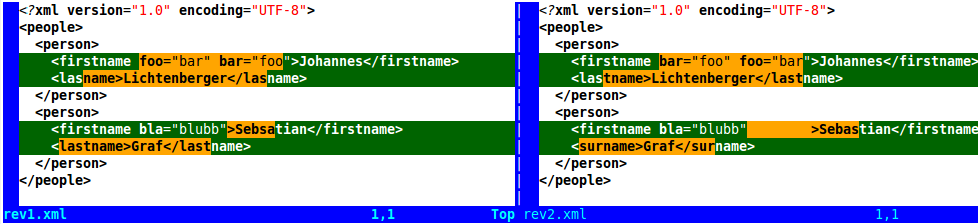
\includegraphics[width=\textwidth]
{figures/gvimdiff.png}}
\caption{\label{fig:faileddiff} GVim diff of two XML-document revisions illustrating the deficiencies of line by line character based diff-tools.}
\end{figure}

\subsection{Problem Statement}\label{subsec::problem}
% Problem statement
%Todays challenges in database research includes the analysis of increasingly large amounts of data. Storing not only one version of a tree-structure but several similar versions proves this task. Analysts typically face the problem of quickly gaining knowledge from a database with potentially large amounts of uninteresting data for the task at hand. They literally have to find a needle in a haystack, which is commonly known as the "information overload" problem. 
Analysts often face the problem of having to compare large tree-structures. While coping with rapidly increasing amounts of data is effectively solved by means of Treetank, comparison requires sophisticated methods on top of it. 

Generally two cases of tree-structures have to be distinguished which our system must be capable of.

\begin{itemize}
\item Tree-structures evolving naturally through applying changes.
\item Similar tree-structures.
\end{itemize}

The research task adressed in this thesis is the problem of how to support analyts in comparing tree-structures .

\subsection{Approach}
% Approach
A promising solution to the task at hand is to use methods from "Visual Analytics", a term coined by James J. Thomas in \cite{VISUAL_ANALYTICS}. Thomas states that Visual Analytics is "the science of analytical reasoning facilitated by visual interactive interfaces.". Thus we provide analytical methods which are inevitable for comparing tree-structures in the first place facilitated by an interactive visual interface. Furthermore interesting patterns can be revealed by custom \texttt{XPath} queries.

Whereas hierarichal visualizations have been studied for some time and sophisticated representations have been found, Visual Analytics of comparing tree-structures just recently gained momentum.

\subsubsection{Value of visualizations}
Francis J. Anscombe reveals the value of graphs (which is generalizable to every (useful) kind of data-visualization) by illustrating in a simple example with four data sets, why graphs are essential to good (statistical) analysis. Using statistical calculations from a typical regression program shows that each computation yields the same result even though fundamental differences are visible on first glance once plotted. Furthermore human brains are trained to interpret visual instead of textual content which is another facet illustrated by this example. It is almost impossible to gain further insights running through the printed out form of these data sets \cite{ANSCOMBE}. 

\subsubsection{Generalization and refinement of our research task}
While several data mining tools are available which specify on specific tasks, tree-structures are flexible and come in many flavors. XML is a meta markup language which is capable of describing all kinds of rooted, labeled trees. Thus it is used by our prototype. In fact it is a semi structured, flexible, meta markup language. XML-documents in stark contrast to relational data do not have to adhere to a schema, which has to be planned and implemented beforehand. Due to that it is mandatory that the visual interface offers great flexibility and thus is not restricted to a special use case.

The high level goal defined in section (\ref{subsec::problem}) can be divided into:
\begin{itemize}
\item Preprocessing and import of differences.
\item Structural comparison based on \texttt{insert-/delete-}operations.
\item Comparison of non-structural data (for instance \texttt{TextNode} values).
\item Extend with \texttt{replace}, \texttt{update} and \texttt{move}-operations (optional).
\item Provide visualizations to quickly gain insights into which subtrees/nodes have been changed.
\end{itemize}

\subsection{Contributions}
The main aim of this thesis is the research and development of an interactive visual interface supporting analysts in comparing tree-structures along with analytical methods to compute the differences in the first place.

In a nutshell this thesis provides the following computer science contributions:

\begin{itemize}
\item Preprocessing of realworld XML data, for instance the revisioned import of (a small fraction of) \emph{Wikipedia} and monitoring changes in a specific Filesystem directory.
\item Several storage-enhancements of a database-system tailored to the storage of temporal tree-structures including compacting, a LevelOrderAxis and new edit-operations to support the implementation of an ID-based differencing algorithm and expressive visualizations. Furthermore a new bulk-insertion operation based on an existing component speeds up hashing of subtrees considerably from $O(n^2)$ to $O(n)$ due to a simple postprocessing postorder traversal whereas $n$ is the size of the nodes in the inserted subtree.
\item Analytical methods (algorithms) to compute structural and non structural differences between similar or evolving tree-structures.
\item Several views:
\begin{itemize}
\item A \texttt{TextView} which serializes an aggregated tree-structure to a syntax highlighted XML output. Furthermore only the visible area plus additionally space to add a slider is filled.
\item A \texttt{SunburstView} facilitating the comparison of tree-structures by a novel layout algorithm and several pruning techniques. Further interaction mechanisms like zooming/panning, a fisheye view, support of XPath-queries and several other techniques are provided as well.
\item A \texttt{SmallmultipleView} supporting different modes (incremental, differential, a hybrid mode).
\end{itemize}
\end{itemize}

\subsection{Conventions}
Pseudocode which is used to illustrate algorithms in this thesis is based on a Java-like syntax as our prototype is based on Java. The following conventions in particular apply:

\begin{itemize}
\item The logical operator \emph{$||$} from Java and other programming languages is denoted by \emph{OR}.
\item Similar the logical operator \emph{$\&\&$} is denoted by \emph{AND}.
\item Variable or reference assignments \emph{$=$} are denoted by \emph{$\leftarrow$}.
\end{itemize}

\subsection{Outline}
The thesis is structured as follows:

\begin{description}
\item[Chapter 2] describes essential preliminaries and provides an overview of algorithms to compute differences in tree-structures. Next, research efforts in visualizing differences of tree-structures are examined. The chapter concludes with a summary of the visualizations which are examined in respect to various attributes.
\item[Chapter 3] starts off with a short description of numerous enhancements to our storage-backend which support an ID-less diffing algorithm as most tree-structures do not use unique node-IDs. The algorithm (FMSE) matches nodes based on similarity-functions for leaf- and inner-nodes in the first place and modifies a tree with as few edit-operations as possible to transform the first tree into the second tree or the first revision/snapshot of a tree into the second in subsequent steps. Next, the implementation of FMSE is described. The algorithm is utilized to import differences stored as snapshots in our storage backend. Once the data is imported a diff-algorithm based on unique node identifiers can be utilized, which is described thereafter. The chapter concludes with performance measures of our node-identifier based algorithm and a short summary.
\item[Chapter 4] is introduced with a short description of a tree-aggregation. Detailed descriptions of our visualizations follow. Furthermore several interaction mechanisms are examined.
\item[Chapter 5] demonstrates the feasability of our approaches based on real world data.
\item[Chapter 6] discusses our approach in relation to the State-of-the-Art.
\item[Chapter 7] summarizes the results and provides suggestions for future work.
\end{description}


 % refer your introduction here
\cleardoublepage
\section{Preliminaries and State-of-the-Art}\label{sec::relwork} %Analysis \& visualization of differences in tree-structured data}\label{sec::hierarichaldata}

\subsection{Introduction}
Today's storage capabilities facilitate the storage of a constantly growing amount of data which is most often collected and stored without filtering or preprocessing.
One of the consequences is the information overload problem defined as:

\begin{itemize}
\item Irrelevant to the current task at hand.
\item Processed or presented in an inappropriate way.
\end{itemize}

To turn these issues into advantages the science called "Visual Analytics" recently became popular. 

James J. Thomas and Kristin A. Cook coined the term "Visual Analytics"\cite{VISUAL_ANALYTICS} and defined it as: "Visual analytics is the science of analytical reasoning facilitated by interactive visual interfaces." It combines (semi-)automatic analytical analysis with interatice visualization techniques, thus emphasizes both cognitive human and electronical data processing strenghts.

Whereas the information seeking mantra is described as "overview first, zoom/filter, details on demand" Keim et al define the Visual Analytics mantra as:

"Analyse First -
Show the Important -
Zoom, Filter and Analyse Further -
Details on Demand"\cite{keim2008visual}

This implies and confirms the important role of humans in the analysis process. As meantioned in the introduction humans are trained to interpret visual impressions but often fail in the same way to construe inappropriate representations (Anscombe's quartet is a very good example).

Our Visual Analytics pipline is largely influenced by the proposal of Keim et al. (depicted in Fig. \ref{fig:visualanalyticsprocess}).

\begin{figure}[htb]
\center{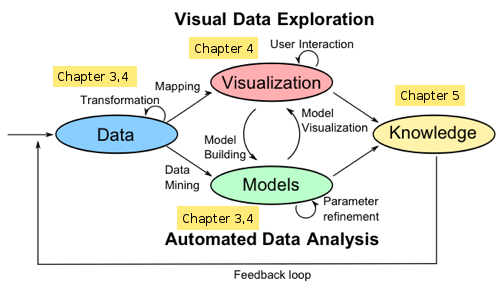
\includegraphics[width=\textwidth - 14em]
{figures/visualanalyticsprocess}}
\caption{\label{fig:visualanalyticsprocess} Visual Analytics Process proposed by Keim et al. Presented in \cite{keim2008visual}.}
\end{figure}

%Chapter \ref{sec::differences} describes the addition of new edit-operations in Treetank and two types of diff-algorithms. These fundamental to analytical reasoning and therefore denote Data Mining methods in Fig. \ref{fig:visualanalyticsprocess}. Models underlying the different views are built based on the output of the the difference-algorithms and thus represent directly the model entity in Fig. \ref{fig:visualanalyticsprocess}. Visualizations (Chapter \ref{sec::visualizations} receive user input and build models through invocation of an ID-based diff algorithm. Parameter changes in the GUI of our main visualization, a Sunburst view tailored to tree-structure comparisons, influence and change the models and in turn change the visualizations according to their output. However user interaction t havet change visualization(s) without having any impact on the model(s).

Comparing tree-structures by a Visual Analytics approach requires analytical reasoning through the computation of differences in the first place. In order to support large tree-structures we decided to use a treebased storage system which is capable of storing transaction-time snapshots efficiently.

\subsection{Storage backend}
Treetank\cite{TREETANK} is an effective and efficient secure storage system tailored to revisioned tree-structures. Currently it supports the import of XML documents which is commonly referred to as \emph{shredding}. To process stored data the W3C recommendations XPath 2.0, XQuery 1.0 and XSLT 2.0\footnote{parts of the XPath 2.0 recommendation have been implemented. Alternatively the Saxon binding can be used which also offers XPath 2.0, XQuery 1.0 and XSLT 2.0 support}, as well as a cursor like Java-API using transactions is supported. Treetank offers a pointer-based encoding and a transaction-based API to navigate in the tree-structure or modify nodes similar to the Document Object Model (DOM\cite{DOM}).

The architecture is based on three exchangeable vertical aligned layers, a transaction-layer, a node-layer and an I/O-layer. It supports \emph{Snapshot-Isolation} through Multiversion Concurrency Control (MVCC) and thus multiple readers in parallel to currently at most one writer. Furthermore the well known ACID properties are supported (Appendix \ref{subsec::acid}). Several consistency checks as of now guarantee well formed XML during serialization. While importing large XMark-instances \cite{XMark} which are commonly used for benchmarking we encountered a space-overhead due to our pointer based encoding. Appendix \ref{subsec::storage} details a number of persistent storage enhancements.

One of the most interesting properties of Treetank for our purpose is \emph{versioning}, that is storing and managing snapshots of tree-structures. Furthermore we utilize hashes which are generated for all nodes during database/resource generation, unique node-IDs as well as query-capabilities. However, Treetank does not provide any information about the changes of a node. The revisioning algorithms merge \emph{NodePage}s, with the same unique ID together and override existing nodes with the latest version. NodePages organize a specified number of nodes in memory. Deleted nodes are introduced to guarantee the correctness after the merge-phase. The combination of NodePages relies on the specific revisioning algorithm. Thus, the merge-phase of NodePages usually refers to the latest full dump of all NodePages or the previous revision. As a direct consequence we are not able to simply utilize the page-layer. However a recent introduction of hook-mechanisms facilitates the indexing of changes to support comparing subsequent revisions (however, not yet implemented). Yet, such an index is only useful for comparing consecutive revisions.

The next section describes a few preliminaries for comparing tree-structures.

\subsection{Analysis of differences}
Line by line textual diffs are based on algorithms which solve the Longest Common Subsequence (LCS) problem. Whereas they are sufficient to track changes in flat text-files, tree-structures need more sophisticated methods as pointed out in the introduction.

The \emph{Extendable Markup Language} (XML) is a textual data format for encoding and structuring documents in machine- and human-readable form. Its inherent data structure is a rooted, ordered, labeled tree. 

\begin{mydef}
A rooted \textbf{tree-structure} is an acyclic connected graph, which starts with a root-node whereas every node has zero or more children and one parent-node with the exception of the root-node. We define a tree $T$ as $T = (N, E, root(T))$ whereas $N$ denotes all nodes, $E$ denotes edges, the relation between child- and parent-nodes and $root(T)$ is the root-node.
\end{mydef}

\begin{mydef}
A rooted, ordered, labeled tree is a tree-structure which extends the rooted tree-definition by defining a specific order for child nodes (that is extending the parent/child edge relation E). Furthermore each node has a label. Thus, $T$ is an ordered, labeled tree, iff $T = (N, E, root(T), \Lambda(n) \in \Sigma)$. $\Sigma$ is a finite alphabet and $n$ is a node in the tree.
\end{mydef}

Thus a tree is more restricted than a hierarchy based on a directed acyclic graph (DAG) in which every node except the root\footnote{which has no parent} has one or more parent nodes.

Many algorithms have been developed to determine differences in tree-structures for instance to provide deltas, which represent a compact version of the changes to the original document.

Next, some essential terms are defined to set the stage for the upcoming sections.

The tree-to-tree correction problem is to determine a (minimal) sequence or set of edit-operations to transform a source tree into a destination tree. 

\begin{mydef}
An edit-operation is an atomar operation which changes a tree.
\end{mydef}

A delta/edit-script is defined as:

\begin{mydef}
A delta/edit-script is a sequence or set of (elementary) edit-operations which when applied to one version v1, yields another version v2.
\end{mydef}

\begin{mydef}
A symmetric delta is a directed delta which is invertible.
\end{mydef}

In the following we use the term \emph{delta} and \emph{edit-script} interchangeably in the generic form meaning directed delta. Each edit operation is usually defined with a fixed cost (usually unit cost).

\begin{mydef}
A minimal edit script is a minimum cost edit script.
\end{mydef}

Besides providing a minimal or close to minimal edit script further metrics of a diff-algorithm are the CPU runtime and the compactness of the delta in terms of storage-space (e.g. it is in most cases sufficient to define edit operations on subtrees, such as a delete- and move-operation which usually removes respectively moves the whole subtree).

Some of the most popular approaches to detect differences in XML-documents which do not require unique node-identifiers (node-IDs) are described next.

\subsubsection{DocTreeDiff\cite{ronnau2009efficient}}
is designed for difference detection in document-centric XML documents. The algorithm computes the Longest Common Subsequence (LCS) on leaf nodes which are on the same level by comparing hash-values. Subsequently ancestor nodes which differ are updated. Then inserted and deleted nodes are determined based on unmatched leaf nodes in the respective tree. As only leaf nodes which are on the same level (number of nodes on the path up to the root node) in the first step are matching candidates, the algorithm does not match identical subtrees if an inner node is added (or a leaf-node is inserted and a subtree is moved and appended to the new node which is sufficient for a tree model which only allows insertions on leaf nodes). Furthermore moves are detected in a postprocessing step instead of on the fly, thus requiring the temporary in-memory storage of inserted and deleted nodes. The runtime complexity is $O(leaves(T)D + n)$ whereas $T$ is the sum of nodes in both trees and $D$ is the number of edit operations and $n$ is the number of non-leaf nodes. The space complexity is $O(T+D)$.%XML documents come in two-flavors. Document-centric XML documents are usually written by an author representing the structure of texts such as website-content or DocBook\cite{DocBook}-based articles whereas data-centric documents are usually automatically created through gathering data. Leaf nodes in document-centric XML usually can be descriminated very well.

%It is stated that document-centric XML typically is restricted in depth by a document format through a Schema or DTD but the width, which grows with increasing text length, is not. Furthermore almost all content is stored in the leafes whereas internal nodes represent the structure of the document (sections, paragraphs, lists, descriptions...). Based on this observation R\"onnau et al. state the following assumptions

%\begin{enumerate}
%\item Content is stored within the leaves.
%\item Changes to structure and markup will be performed on a higher level within the tree.
%\item Many non-leaf nodes are equal due to identical markup.
%\end{enumerate}

%Based on these assumptions the algorithm relies heavily on the computation of a LCS on leaf nodes.

%\begin{enumerate}
%\item First the algorithm computes the LCS on leaf nodes based on their hash values and the depth in the tree.
%\item Next, a bottom up traversal of all leaf nodes which are considered equal follows to detect updates for each anchestor node. All nodes are marked which have been processed to skip the process for subsequent bottom-up traversals when an anchestor node is the same.
%\item Last, deletes, inserts and moves are detected. A second bottum up traversal starting at leaf nodes which have not matched, detects nodes which are in the old revision but not in the new are considered as being deleted. At every level the child nodes of the parents are searched for the neares node which has been marked as matched during the LCS computation. If one is found the traversal stops. The same holds for inserted nodes if the reverse condition is true. Therefore the bottom-up traversal detects the largest possible subtrees to delete or insert, since the edit operations are not defined on single nodes. Furthermore adjacent deletions or insertions are glued together. Delete/insert-operations on the same subtrees are combined into one move-Operation.
%\end{enumerate}

\subsubsection{DeltaXML\cite{DELTAXML}}
Nodes are matched according to their type, the level in the tree and the Longest Common Subsequence (LCS). Furthermore matching PCDATA nodes are optionally prefered. Similar, attribute-IDs in the deltaxml-namespace may be used to mark nodes with unique IDs. Marking all nodes with an ID generates a minimum edit script. However, a complete description of the algorithm is not published.

\subsubsection{XyDiff\cite{cobena2002detecting}}
Cobena et al. present in \cite{cobena2002detecting} a fast heuristic algorithm in the context of Xyleme, an XML database warehouse. %Initially a unique persistent identifier XID is assigned to each node. XID-Maps are generated through a postorder traversal whereas initially integers from 1 to n are assigned. N denotes the number of nodes in the original tree. Added nodes in the revision to compare are assigned further integers starting from n + 1 again by a postorder traversal. Nodes which are not present in the new revision are removed resulting in gaps. Assuming an initial range of identifiers from (1-474) it might result in several ranges, for instance (1-13),(17-447),(450-474) which means that the nodes with the XIDs 14, 15 and 16 have been deleted as well as the nodes 448 and 449. The algorithm for the actual change detection is outlined in the next paragraph. Inserts, Deletes, Updates and Moves are supported. 
Signatures which are hash-values computed based on the value of the current node and all child signatures are used. Inserts and deletes are restricted to leaf nodes in the spirit of Selkow's tree-model \cite{tai1979tree}. Based on heuristics large subtrees are matched and depending on weights propagated to parent/ancestor nodes. In \cite{ronnau2009efficient} several deltas are examined whereas the greedy subtree-algorithm yields large deltas. However, tuning parameters as the weights and how far to go up to match parent nodes is not considered.

%First nodes with ID attributes defined in a DTD are matched. Then signatures are generated in a bottom-up traversal, which are hash values computed from the value of the current node and all child signatures. Furthermore weights are computed and defined as the text node sizes which are summed up for each child node. A priority queue is build, whereas the largest weights of the new document are prioritised. The largest subtrees are considered first to be matched based on their signatures. If more than one node has the same signature a heuristic is used, otherwise the child nodes are added to the queue. Whenever nodes match each subtree and anchestor pair is going to be matched as long as the labels are equal. The propagation to anchestor nodes depends on the node weight. A heuristic is used to substitute the computation of largest order preserving common subsequences for the move-operation. As heuristics are used the resulting edit-scripts/deltas are not guaranteed to be minimal.

The CPU runtime of the algorithm is $O(n \log n)$ and the space complexity is $O(n)$ whereas $n$ is the size of both documents.

\subsubsection{LaDiff / Fast Match Simple Editscript (FMSE)\cite{chawathe1996change}}\label{subsec::ladiff}
operates on different versions of LaTeX documents. We describe the algorithm in slightly more detail as we decided to implement the algorithm for XML data in Treetank. It is developed in the context of \LaTeX to demonstrate and measure the feasibility of an approach to detect changes in hierarichally structured information. 

Chawathe et al. divides this task into two main problems:

\begin{description}
\item[the Good Matching problem] is the problem of finding matches between the two trees, which are either equal for some predefined function or approximately equal.
\item[finding a Minimum Conforming Edit Script (MCES)] is the second obstacle. Recapitulate that an \emph{edit script} is a sequence of edit operations transforming the source file into the target document once applied. Costs are therefore applied to every edit operation.
\end{description}

The algorithms used to solve these two problems operate on rooted, ordered, labeled trees. Four edit operations (\texttt{insert}, \texttt{delete}, \texttt{update} and \texttt{move}) are defined with unit costs such that an \texttt{insert}/\texttt{delete} or \texttt{delete}/\texttt{insert} is more costly than a \texttt{move}.

The algorithm proves to yield minimum edit scripts in case the assumption holds true that no more than one leaf node is considered equal to a predefined function which compares the values of leaf nodes and the labels match. XML does provide labels in form of \texttt{QName}s for \texttt{element}- and \texttt{attribute}-nodes (as well as attribute-values) and a slightly restricted alphabet for \texttt{text}-nodes. Thus either text-node values have to be compared, \texttt{QName}s or \texttt{QName}s and attribute-values.

The first criterium defined for leaf-nodes is 

\begin{equation} 
compare(v(x), v(y)) \leq f\ such\ that\ 0 \leq f \leq 1
\end{equation}

Inner nodes are matching candidates according to

\begin{equation}
\frac{|common(x, y)|}{max(|x|,|y|)} > t\ and\ label(x) = label(y)
\end{equation}

\begin{equation}
common(x,y) = \{(w,z) \in M | x\ contains\ w\ and\ y\ contains\ z\}
\end{equation}

whereas a ``node x contains a node y, iff y is a leaf node descendant of x and $|x|$ denotes the number of leaf nodes x contains''. The threshold t is defined as $0.5 \leq t \leq 1.0$.

In a first step the good matching problem is solved by means of concatenating nodes/labels bottom up during a postorder traversal and finding a longest common subsequence (LCS). Furthermore, nodes which are unmatched during the LCS-matching are subject to a subsequent comparison. The predefined similarity-function is applied and if the nodes are matched they must be aligned. 

After that in a breadth first traversal nodes are inserted, updated or moved. The children of each node are aligned based on the LCS once again. Nodes which are matched but not in the LCS are moved. The order in which operations are applied to the source tree and the edit script is crucial to the correctness of the algorithm. Details are omitted for brevity.

The second step is the deletion of unmatched nodes during a postorder-traversal.

When the assumption which assures the generation of a minimum edit-script does not hold which might be the case for several XML-documents, especially in data centric XML files, the algorithm yields large output-deltas due to mismatches according to Lindholm et al.\cite{lindholm2006fast} and Rönnau et al.\cite{ronnau2009efficient}. This is a direct consequence of the ambigiouty of the LCS as well as of the subsequent matching of nodes. However this is a problem common to almost all differencing algorithms and can be minimized by proper definitions of the similarity functions for leaf- and inner-nodes. An optional postprocessing step reduces mismatches and thus move-operations such that children of matched nodes, which do not have same parent are candidates for matches with children of the same parent in the other tree, thus correcting some misaligned nodes. Note that this step can not reduce errors, which are propagated from mismatched leaf nodes.

It becomes apparent by investigating the analysis of Rönnau et al.\cite{ronnau2009efficient} that the result of mismatched leaf-nodes in contrast to other algorithms yields many moves (compared to more inserts/deletes in other algorithms). However, moves in Treetank without generating hashes and storing the number of descendants of each node during import are a constant time ($O(1)$) operation due to the pointer-based approach. Even with hashing enabled which provides inevitable performance-boosts for our internal ID-based diffing algorithm which is used in a subsequent step by our visualizations, only ancestor nodes are affected and thus linear time is needed (however much faster than a deletion and insertion which in addition requires traversing the whole subtree two times).

The runtime complexity is $O(n*e+e^2)$ and the space complexity is $O(n)$ whereas $n$ is the number of unchanged nodes and $e$ is the number of different/changed nodes.

\subsubsection{X-Diff\cite{wang2003x}}
operates on unordered, labeled trees. Thus the order of child nodes does not matter. Despite using an unordered tree-model which is not suitable in many cases as for instance document centric XML, updates on element nodes to the best of our knowledge are not defined as the signature for \texttt{TextNode}s does not use their values. However updating an internal node is crucial due to otherwise potentially large subtree delete- and insert-operations even though only a single node is updated.

%First XHash values are computed in a bottom up postorder traversal for every node which represent the entire subtree rooted at the respective node.
%The hash computation does not include the child order, such that isomporhic trees can be matched in subsequent steps.

%Next the trees are traversed starting from the root-nodes. Nodes on currentLevel+1 are filtered out which have equal hash values.

%Signatures defined as $Signature(x) = /name(x_{1})/.../name(x_{n})/name(x)/type(x)$ for element nodes and $Signature(x) = /name(x_{1})/.../name(x_{n})/type(x)$ for text nodes are used to determine if nodes are considered to match. Note that in case of a text node it does not contain the value in the signature. This decision leads to the support of update-Operations, which are only defined as an edit cost for text nodes. 

%Initially leaf nodes are compared based on a predefined edit distance function and a matching/distance-value tuple is stored in a table. To compute the edit distance between subtrees the minimum-cost maximum flow algorithm \cite{zhang1996constrained} is used.

%Based on a minimum cost matching and the distance table an edit script can be computed.

The runtime is defined for three involved steps separately: 

\begin{enumerate}
\item {\bf{Parsing and Hashing}}: $O(|T_{1}| + |T_{2}|)$
\item {\bf{Mapping}}: $O(|T_{1}| \times |T_{2}|) \times max\{deg(T_{1}, deg(T_{2})\} \times \log_{2}(max\{deg(T_{1}), deg(T_{2})\}))$
\item {\bf{Generating Minimum-Cost Edit Script}}: $O(|T_{1}| + |T_{2}|)$
\end{enumerate}

\subsubsection{Faxma\cite{lindholm2006fast}}
uses fast sequence aligning transforming the parsed documents into sequences of tokens. Subsequently the diff is computed using rolling-hashes with different window-sizes. Moves are handled through the combination of \texttt{delete/insert} pairs which is similar to the approach used by \emph{DocTreeDiff}. The delta is a script which includes identifiers to matched nodes with inserted sequences in between. It is thus not defined in terms of a usual edit script and therefore not directly useful for our purpose.   %First the input documents are parsed into XAS tokens, which preserves the XML structure. They support three edit operations: \texttt{insert}, \texttt{delete} and \texttt{move} since they claim that subtrees are often moved. . Based on \emph{rolling-hashes} a sliding window iterates over sequences derived from transforming both XML documents. A rolling-hash can be updated really fast if the right hash-function is chosen. If so, only the old value, the new value and the previous hash-value is needed \cite{RollingHash}:

%\begin{equation}
%h(S_{i+1}) = H(h(S_{i}), s_{i} , s_{i+n+1})
%\end{equation}

%To quickly find maximum length matches, window sizes of length $S = <48,32,16,8,4,2,1>$ are used.

%At first all nodes are marked as $ins(node)$ in both sequences. Starting with the greatest size, matches are searched for in a zigzag-pattern, whereas matched sequences are extended alternately moving forward and backward until no further matches are found. These matches are marked with\\ $cpy([start\ index], [end\ index])$ in the sequence of the updated document. Any matching sequences are then removed from the sequence representing the old revision, finally resulting in the configuration, that only deleted nodes are left in this sequence.

%Since the matches are not necessarily aligned on subtree boundaries the match-list must be transformed back into the tree-domain.

%The algorithm serializes match lists in a sequential traversal, providing the \texttt{start-} and \texttt{end-tag} has been encountered. A queue of tentative node- and tree-reference tags is maintained to either discard changes partially or serialize the results. Details of this algorithm are omitted, since the resulting delta does not fit our purpose. The delta is a script which includes identifiers to matched nodes with inserted sequences between. It is thus not defined in terms of an edit script and thus not directly useful for our purpose.

\subsubsection{Summary}
The problem in common to all approaches is to efficiently compute a minimum or near minimum edit script in order to transform the first into the second tree. Unfortunately a guaranteed minimum edit script for the the tree-to-tree correction problem is known to be bound in runtime by \\$O(nm\ min(depth(T1),\ leaves(T1))\ min(depth(T2),\ leaves(T2)))$, with $n$, $m$ denoting the number of nodes of the trees $T1$ , $T2$\cite{Zhang:1989:SFA:76071.76082}. Using heuristics speeds up the process but in most cases generates non optimal (non minimal) edit scripts. These non minimal deltas are counterintuitive when used to determine differences between tree-structures, because of mismatched nodes. These mismatches result in modifications of nodes which should not be changed and vice versa. However detecting changes is not our primary obstacle, which requires monitoring. Even algorithms which guarantee a minimum edit script do not necessarily reflect the changes due to their inherent ambiguity. Usually a few edit-scripts are minimal according to their cost-model of edit-operations.

Every diff-algorithm has its strength and pitfalls. Depending on the input and expected modification patterns some algorithms provide better results than others in terms of predefined evaluation criterias. Even though several algorithms are compared in \cite{ronnau2009efficient} we remain critical as the size of the delta and the amount of edit-operations might not be the best descriminators. The granularity and the cost of edit-operations is equally important. For instance the cost of the moves in Treetank at worst is linear in the number of ancestor nodes, the sum of ancestors of the node before it is moved and afterwards and constant at best, depending on configuration options\footnote{generating hashes and determining the number of descendants of each node or not}. Defining insertions and deletions in terms of subtrees reduces the size of the edit-script. However it does not take the cost of applying these changes into account. That said all algorithms work best if leaf-nodes are distinguishable very well and thus the similarity measures are able to match only one node in the other tree. Otherwise finding a best match for each node results in at least a quadratic runtime. Comparing document oriented XML thus usually produces better results in comparison to data centric XML in terms of minimum or near minimum edit-scripts/deltas.

Memory consumption is very important considering large XML instances ranging from 10 MiB to 100 MiB and more. However at some point either the trees have to be splitted or costly I/O operations due to serialization/deserialization of datastructures on external storage have to be used. Reducing the cost of computing the LCS which has a large memory footprint might be mandatory but also results in heuristics. A survey of the wide range of algorithms is summarized in \cite{cobena2002comparative}. Several algorithms are described and compared according to the attributes memory consumption, time complexity, supported operations and the tree model. However it does not include comparisons of recent algorithms as DocTreeDiff and Faxma. Thus, a short summary is detailed in Table \ref{chap2:comparsion}. DeltaXML 

In summary a trade-off between the number of edit-operations, the memory consumption and the runtime complexity of the algorithm exists. Furthermore no algorithm exists which outperforms and in respect to the edit-script cost produces always better results than the others while comparing trees of different domains and characteristics. It heavily depends on the change pattern of the input document and parameters of the algorihm if provided. Due to the different granularity of the edit-operations among the approaches the size of the delta and the number of different types of edit-operations is not always a good evaluation critera. To be fair the cost of applying all edit-operations must be determined. Thus, the cost of insertions and deletions is always defined on the subtree-sizes.

\begin{table}[tb]
\centering 
\begin{tabular}[r]{|l|c|c|c|c|} 
\hline
\textbf{algorithm} & \textbf{runtime} & \textbf{space} & \textbf{tree model} & \textbf{move support}\\
\hline
\hline
\textbf{DeltaXML} & not published & not published & not published & not published\\
\hline
\textbf{XyDiff} & $O(n \log n)$ & $O(n)$ & ordered & yes\\
\hline
\textbf{FMSE} & $O(n e + e^2)$ & $O(n)$ & ordered & yes\\
\hline
\textbf{X-Diff} & $O(n^2)$ & not published & unordered & no\\
\hline
\textbf{DocTreeDiff} & $O(leaves(T)D + n)$ & $O(T+D)$ & ordered & yes\\
\hline
\textbf{Faxma} & $O(n)$ (average) & not published & ordered & no\\
& $O(n^2)$ (worst) &  & & \\
\hline
\end{tabular}
\label{chap2:comparsion}
\vspace{0.5em} 
\caption{Comparsion of tree-to-tree difference algorithms.}
\end{table}

\subsection{Visualization of differences}
In the past several visualization techniques have been proposed for hierarichal data ranging from simple node link diagrams, force directed layouts to space filling approaches. Comparison of tree-structures just recently gained momentum. %Recently database systems which are capable of storing hierarichal temporal data efficiently and therefore store snapshots of time varying data put forth the need to analyse these data. %to determine and visualize changes between several revisions such that analysts are able to answer time dependent questions like the ones raised in the motivating application examples.

%While in the past it has been possible to map temporal hierarichal data to relational databases it required the storage of a full snapshot through foreign/primary key relations instead of just storing incremental or differential updates as well as the hierarichal mapping overhead.

%\subsubsection{TimeRadarTrees\cite{vilanovatimeradartrees}} To visualize weighted dynamic compound Digraphs, which are graphs with a hierarichal dimension, TimeRadarTrees have been developed. Changes of leaf nodes and their directed edges are revealed, whereas incoming edges are plotted in a radial manner as a slice on the inner circle. Outgoing edges are represented by the outer thumbnails. Therefore visual clutter regarding related nodes, which occurs in node link diagrams is avoided. The hierarchy and thus the inner nodes are drawn on top of the inner radial circle (Fig. \ref{fig:timeradar}). The leaf nodes are labeled A, B, C, D and E. Each segment of a node represents the node in a specific revision of the graph. Node D has three incoming edges in the first graph, in the second one and in the third none (inner circle). The color red denotes that the node has at least one incoming or outgoing (which depends on wether one looks at the inner or outer circles) edge. Grey scale means the node has no incoming/outgoing edges at all. As TimeRadarTrees visualize changes on leaf nodes but not the hierarchy itself they ca not be directly mapped to our task and thus are not present in the short evaluation at the end of this chapter and in table \ref{chap2:comparsion}.

%\begin{figure}[tb]
%\center{\includegraphics[width=\textwidth - 12.5em]
%{figures/timeradar}}Phylogenetic trees among a nontrivial number of input sequences are constructed using computational phylogenetics methods. Distance-matrix methods such as neighbor-joining or UPGMA, which calculate genetic distance from multiple sequence alignments, are simplest to implement, but do not invoke an evolutionary model. Many sequence alignment methods such as ClustalW also create trees by using the simpler algorithms (i.e. those based on distance) of tree construction. Maximum parsimony is another simple method of estimating phylogenetic trees, but implies an implicit model of evolution (i.e. parsimony). More advanced methods use the optimality criterion of maximum likelihood, often within a Bayesian Framework, and apply an explicit model of evolution to phylogenetic tree estimation.[3] Identifying the optimal tree using many of these techniques is NP-hard,[3] so heuristic search and optimization methods are used in combination with tree-scoring functions to identify a reasonably good tree that fits the data.
%Tree-building methods can be assessed on the basis of several criteria:[6]
%\caption{\label{fig:timeradar} TimeRadarTrees illustration. Presented in \cite{vilanovatimeradartrees}.}
%\end{figure}

\subsubsection{Treevolution\cite{theron2006hierarchical}} visualizes the evolution of hierarchical data in a radial node-link diagram. Each node might have arbitrary many parent nodes and each ring represents one snapshot of the hierarchy. Inserted nodes are placed on the appropriate ring depending on the time of insertion. However edge crossings occur frequently due to the parent-child relationship whereas often times nodes have more than one parent. A direct consequence is visual clutter which complicates the analysis of the hierarichal relationship between inserted nodes and their parents. Furthermore label overplotting occurs frequently which is a result from drawing the labels in one direction (left to right), however a simple interaction method improves on this by providing rotation mechanisms.

\subsubsection{Interactive Visual Comparison of Multiple Trees\cite{bremm2011interactive}} The authors propose a prototype to compare multiple phylogenetic trees. Several views are available to analyse the trees on different levels of detail. A matrix view for instance displays pairwise tree-similarities based on a similarity score which takes overlapping subtrees into account. The similarity score depends on all nodes in a subtree including inner nodes instead of just determining overlapping leaf nodes. A histogram shows the score distribution among all nodes in all trees. The consensus tree is "a compact form of representing an 1:n comparison" in one tree. The score is "the average of the scores comparing a reference tree node against its best matching unit in all other trees". The last view is a Tree Comparison View which highlights all nodes in the subtree a user marks through a linking and brushing technique in all other trees. It is the only system which is capable of comparing multiple trees on different levels of detail at the same time with linked visualizations. However we assume that the quadratic runtime of comparing all nodes with all other nodes will be restricted to (many) small trees. Furthermore to the best of our knowledge it is not meantioned how nodes are compared, but we assume unique labels or node identifiers are required as the prototype is proposed for phylogenetic trees. 

\subsubsection{Spiral-Treemap/Contrast-Treemap\cite{tu2007visualizing}}
A Treemap is a space filling approach which maximizes available screen space for the visualization. Most treemap layouts suffer from abrupt significant layout changes even if the underlying data changes were rather small. Tu et al. propose a new layout algorithm called \emph{Spiral Treemap} to improve the layout stability arranging child nodes in spirals which change the orientation by 90° in the corners. Child-nodes are aligned along a spiral in each level beginning at the upper left corner. Therefore edit-operations as for instance \texttt{inserts} and \texttt{deletes} only affect local regions. However, we argue that it is not trivial to analyse strutural differences as they are not explicitly visualized in the Contrast Treemap and the texture distortion depends on the layout algorithm, whereas small changes are hardly visible. Furthermore the hierarchy is not easy to recognize in the Spiral Treemap which is a common problem for Treemaps owed to the enclosing nature of child nodes in their parent nodes. Labels however are easily perceived if the rectangles are not too thin which occurs frequently in large trees ranging from about $50000$ nodes to a few hundred or even millions of nodes. Furthermore the nodes degenerate from rectangles to very tiny stripes. Improving the aspect ratio of the rectangles results in Squarified Treemaps\cite{bruls2000squarified}, which lack the property of ordered siblings. However child-nodes in trees are often ordered which is why Squarified Treemaps in general are only feasible in certain specific cases which lack a semantic difference in node ordering. %(Fig. \ref{fig:treemap-spiral}). Furthermore \emph{Contrast Treemaps} are proposed to visualize attribute changes. First a union tree is build to merge the two trees. Inserted and Deleted nodes are missing the corresponding attribute value in the other tree. Otherwise two attribute values are available from each tree, which are color coded in the same rectangle. The value of the "original" item is in the top left corner whereas the other value is in the bottom-right. Additionaly it is possible to encode the value depending on the occupied area. The higher the value in one tree the more area is occupied, the lower the value the fewer area is utilized. The Spiral Treemap layout algorithm is used whereas the size of the items in the Treemap is based on one of the attribute values or an aggregation function (min, max, avg). Another technique helps tracking layout changes. A background image is placed behind one of the two Treemaps representing one of the trees. It is distorted in regions which have changed due to the second Treemap layout. Regions which are extended or shrinked are also reflected in the distortion of the background image. Note, that in order to gain knowledge from the distorted texture/image a stable layout algorithm as for instance the Slice and Dice or Spiral Treemap is required. 

%\begin{figure}[tb]
%\center{\includegraphics[width=\textwidth]
%{figures/treemap-spiral}}
%\caption{\label{fig:treemap-spiral} Spiral Treemap. Presented in \cite{tu2007visualizing}.}
%\end{figure}



%\begin{figure}[tb]
%\center{\includegraphics[width=\textwidth]
%{figures/treevolution}}
%\caption{\label{fig:treevolution} Treevolution. Presented in \cite{theron2006hierarchical}.}
%\end{figure}

\subsubsection{TreeJuxtaposer\cite{munzner2003treejuxtaposer}}
TreeJuxtaposer is a system designed to support biologists to compare the structures of phylogenetic trees. A new comparsion algorithm to determine matching nodes in near-linear average time is proposed. Perfect matching nodes have the same labels for each of their leaf nodes. Based on a simple similarity measure ($S(A,B)$ between two sets whereas the function is defined as $\frac{A \cup B}{A \cap B}$) they propose a method to colorize edges of non perfectly matching nodes and a rectangular magnifier to emphasize changed nodes. The visualization itself contains several revisions side by side plotted in node-link diagrams. Selections and rectangular magnifications are synchronized. TreeJuxtaposer uses a node-link algorithm and thus shares the drawbacks of other node-link visualizations such as \emph{Treevolution} and the \emph{Ripple presentation}. In comparison to space filling approaches further attributes as for instance value comparisons, subtreesizes and labels are not visualized or result in visual clutter. Furthermore the fast differencing algorithm to the best of our knowledge relies on unique node labels to support the region query on a two-dimensional plane.

%\begin{figure}[tb]
%\center{\includegraphics[width=\textwidth]
%{figures/treejuxtaposer}}
%\caption{\label{fig:treejuxtaposer} TreeJuxtaposer. Presented in \cite{munzner2003treejuxtaposer}.}
%\end{figure}

\subsubsection{Code Flows: Visualizing Structural Evolution of Source Code\cite{telea2008code}}
Code Flows is proposed for determining and tracking changes in source code between several revisions. It is a space filling approach which uses horizontally mirrored icicles and therefore additional attributes of nodes are visualizable besides highlighting actual tree changes. Labels are readable in smaller trees or when zoomed in because of the rectangular layout of icicle plots. Due to spline-tubes matching, nodes can be tracked very well through different revisions. Even code splits and merges are easily trackable. On the downside small code changes resulting in the addition or deletion of a few nodes might not be visible at first glance. Furthermore the spline connections between matched nodes leads to visual clutter due to overplotting when nodes are moved.

%\begin{figure}[tb]
%\center{\includegraphics[width=\textwidth - 15em]
%{figures/codeflows}}
%\caption{\label{fig:codeflows} Code Flows. Presented in \cite{telea2008code}.}
%\end{figure}

\subsubsection{Ripple presentation for tree structures with historical information\cite{ishihara2006ripple}}
The Ripple presentation visualizes both evolving hierarchies and categories. Concentric circles are used to indicate an evolving hierarchy through time. Each circle represents one point in time. Nodes are plotted in a special node-link layout. The root node of each subtree is in the focus of the view. Leaf nodes are arranged in ascending order meaning older nodes are drawn on circles further away from the current root of the subtree. The angles of edges are application dependent and facilitate the clustering of categories through time. In their news articles, example categories are extractable from the content. For each child belonging to the same category the angle of the edge has to be located in between the parent angle. Since the application examples require no diff-calculation and updates as well as deletions of nodes are not considered it is not useful to compare every aspect of changing tree structures. It suffers from a lot of clutter consequent to label overplotting as well. Deletions and updates have not been considered since the example use cases to the best of our knowledge just add nodes and categories. Due to the fact that it is also a node link representation and not a space filling approach attributes of nodes are not visualizable. Thus it is best comparable to Treevolution, but because of the more complex layout algorithm it can group nodes according to categories. 

%\begin{figure}[tb]
%\center{\includegraphics[width=\textwidth - 12em]
%{figures/ripple}}
%\caption{\label{fig:ripple} Ripple presentation. Presented in \cite{ishihara2006ripple}.}
%\end{figure}

\begin{table}[tb]
\centering 
\begin{tabular}[r]{|l|c|c|c|c|} 
\hline
\textbf{visualization} & \textbf{hierarchy} & \textbf{space filling} & \textbf{readability} & \textbf{changes}\\
\hline
%\hline
%\textbf{Sunburst} & +++ & ++ & + & +++\\
\hline
\textbf{Spiral-/Contrast-Treemap} & + & ++\footnotemark & ++ & ++\\
\hline
\textbf{Treevolution} & + & - & + & +\\
\hline
\textbf{Code Flows} & +++ & ++ & ++ & ++\\
\hline
\textbf{Juxtaposer} & ++ & - & ++ & +++\\
\hline
\textbf{Ripple Presentation} & + & - & + & +\\
\hline
\textbf{IVCoMT} & +++ & - & ++ & ++ \\
\hline
\end{tabular}
\label{chap2:comparsion}
\vspace{0.5em} 
\caption{Comparsion of tree-to-tree comparison visualizations. "-" indicates the absence of an attribute, "+" to "+++" implies how well or bad the attribute is supported.}
\end{table}

\footnotetext{due to the side by side view which needs a lot of space}

\subsubsection{Summary}
Recently, interactive visualizations of the evolution of tree-structures or different, similar trees have been proposed. Table \ref{chap2:comparsion} summarizes the visualizations according to several attributes. The first column denotes the readability of the hierarchy-representation. The second column indicates if a space filling approach is used and to which extend the whole display space is utilized. The third column characterizes the readability of the visualization including the encoding of differences and labels. The last column is the most significant. It determines to which extent changes are visualized. Even deletions are not considered in some cases which might be due to the use cases of the respective visualization. Note that the scala range from "-", not present to "+++" (best). Chapter \ref{sec::conclusion} presents a detailed more comprehensive analysis in comparison to our system. 

Most of the visualizations are tailored to specific tasks and thus are at best only partially useful for other applications. In fact besides adapting the diff-algorithm described in \cite{telea2008code} none of the proposed systems to the best of our knowledge is able to compare every kind of tree structure due to diff-algorithms which rely on domain characteristics as unique node identifiers/node labels or on change detections which hook into a system. Furthermore we suppose that except TreeJuxtaposer and CodeFlows no other system is able to compare large trees. However, in CodeFlows the filtering of nodes depends on the level of detail (per class-level, function-level...). Thus a global view which filters all relevant, changed nodes is not available.

The prototype presented in \cite{bremm2011interactive} by Bremm et al. is the only system capable of visualizing differences at various levels of detail due to linked visualizations. However, we are observe, that the approach in its current form is not applicable to large tree-structures due to their similariy measures which pose a quadratic runtime complexity.

%The use cases of \emph{TimeRadarTrees} are rather different from the ones addressed in this thesis. While changes of leaf nodes and the relationships between them are in the focus of TimeRadarTrees, determining and visualizing changes of the whole hierarchy is one of the main goals in this thesis.



%\emph{Ripple presentations} 

%\begin{figure}[tb]
%\center{\includegraphics[width=\textwidth - 12em]
%{figures/ripple-clutter}}
%\caption{\label{fig:ripple-clutter} Ripple representation - label overplotting. Presented in \cite{ishihara2006ripple}.}
%\end{figure}

%\emph{TreeJuxtaposer} 

%\emph{Code flows}

%\emph{Interactive Visual Comparison of Multiple Trees} 






 
\cleardoublepage
\section{Analysis of structural differences}\label{sec::differences}
\subsection{Introduction}
This chapter describes the implementation of an algorithm which does not rely on unique node identifiers (FMSE, described in general in Chapter \ref{sec::relwork}, Section \ref{subsec::ladiff}) as well as a new ID-based algorithm which utilizes a preorder traversal on both trees to compare tuples of two nodes each time. The FMSE algorithm facilitates the import of differences between two tree-structures which do not incorporate unique node-IDs in the first place either to compare different, similar tree-structures or the evolution of a tree. Thus, our similarity measures are based on the tree-to-tree correction problem. The visualizations proposed in the next chapter rely on the diff-algorithms described in this chapter which detect edit-operations/diff-types to transform a source tree into a target tree. A reference tree is initially imported in Treetank, our storage backend. Subsequently, changes between this tree and either other trees or the evolution of the reference-tree in terms of edit-operations are stored as subsequent revisions. As described in the last chapter, the Fast Matching Simple Edit-Script algorithm depends on similarity-measures and does not require nor use unique node-IDs in our case. Thus, a minimum edit-sequence usually is not guaranteed if leaf nodes are very similar. While importing the differences through FMSE, the storage system Treetank assignes unique stable node-IDs which are subsequently utilized by our ID-based diffing algorithm to support a fast linear-runtime difference-computation.

During the import of collections, that is either multiple revisions of one tree or different similar trees, changes are computed by comparing the latest stored revision in the database backend with either the next tree-revision or (similar) tree to import. Once imported, unique node-IDs and optionally hashes facilitate a new fast diff-algorithm. Diff-tuples are generated by comparing two nodes each time. They include the type of difference, the compared nodes and their depth in the tree and facilitate an aggregated tree-structure made up of both changed- and unchanged-nodes through collecting the diff-tuples in the model of a visualization as described in the next chapter (Chapter \ref{sec::visualizations}). 

%\begin{figure}[tb]
%\centering
%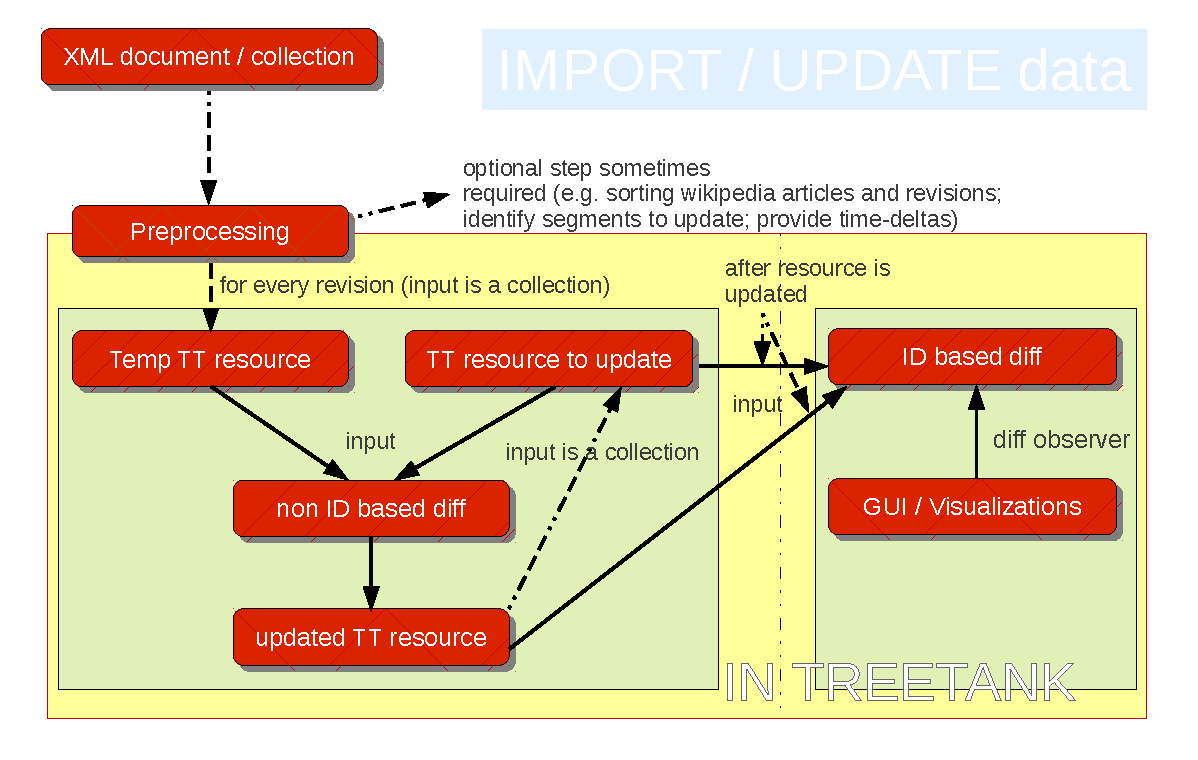
\includegraphics[width=\textwidth]{figures/importdata}
%\caption{Importing differences encountered through the FMSE ID-based diffing-algorithm.} 
%\label{fig:importdata}
%\end{figure}

Both algorithms, the FMSE algorithm, which does not require unique node-IDs, used for importing differences and the fast ID-based diff-algorithm are implemented using Treetanks' transaction-based Java-API, the native secure tree-storage system, which is used as an integral part to demonstrate our approach. First, preliminaries such as new edit-operations required for implementing the FMSE-algorithm and a compact, meaningful aggregated tree-structure are described. Note that a rich set of edit-operations facilitates an expressive visualization. It is a lot more intuitive and meaningful to provide atomar \texttt{replace}- and \texttt{move}-operations to reflect changes between tree-structures than using combinations of \texttt{delete}- and \texttt{insert}-operations and thus losing any association. Once, having described preliminaries the implementation itself is sketched. A description of our internal ID-based diffing algorithm follows. The chapter concludes by analysing the asymptotic bound of the algorithm both in terms of the runtime as well as the space consumption and synthetic, empirical benchmarks which confirm the scalability of our algorithm.

%\subsection{Storage backend}
%Treetank is an effective and efficient secure storage system tailored to revisioned tree-structures. Currently it supports the import of XML documents which is commonly referred to as \emph{shredding}. To process stored data the W3C recommendations XPath 2.0, XQuery 1.0 and XSLT 2.0\footnote{parts of the XPath 2.0 recommendation have been implemented, alternatively the Saxon XPath 2.0 binding can be used which also offers the XQuery 1.0 and XSLT 2.0 support}, as well as a cursor like Java-API using transactions is supported. The architecture is based on four exchangeable vertical aligned layers. The following is a brief description of each layer in a top-down approach:

%\begin{description}
%\item[Transaction] Transactions are divided into \texttt{read}- and \texttt{write}-transactions. Read-Transactions are able to read stored nodes through a cursor-like API. Write-Transactions extend the functionality of Read-Transactions and provide both read- and write-semantics. They aditionally provide methods to modify data and commit the changes to store a new revision. Changes are atomar and saved in a transaction log which literally means they are either commited at a whole or aborted and rolled back. All ACID-properties are supported. Commiting changes results in a new appended revision, whereas nodes internally are stored based on a copy-on-write (COW) principle and a revisioning approach (full, incremental, differential and a new sliding-window\cite{kramis2009} based hybrid). Aborting a transaction means that all modifications issued during the transaction after the last commit are not persisted and lost. Update operations are applied immediately in main-memory but saved in a transaction log which is used to persist the changes after a commit. Consistency rules apply either at pre-commit time or at the time a transaction is commited.

%Every transaction includes a unique transaction ID as well as a timestamp which denotes the last commit-time of the transaction.

%\item[Node] The node layer is responsible for providing different node kinds. Currently \texttt{comment} and \texttt{processing-instruction} nodes are not supported due to the prototype research state of Treetank which is sufficient in almost all cases. Note that adding these two node types in general is straight forward. The node- and transaction-layer are responsible for the storage encoding. The main focus of the node-layer is the update-performance. Thus the pointers are stored eventuating in a local \\\texttt{key/parentKey/firstChildKey/[left|right]SiblingKey} encoding illustrated in Fig. \ref{fig:encoding}. The dashed lastChild pointer currently is not available but may be added to support efficient XPath-queries as for instance the \texttt{fn:last()}-function to get the last-element in a context-set. 

%Inserting a structural node either involves calling \texttt{insertAsFirstChild()} or \texttt{insertAsRightSibling()} on a write transaction. The first case requires to set

%\begin{itemize}
%\item the parent key to the current key located at the current transaction cursor position (before the insert)
%\item a special \texttt{NULL\_NODE\_KEY} to mark the nonexistence of any left sibling
%\item the former first child as the right sibling
%\end{itemize}

%The latter case requires to set

%\begin{itemize}
%\item the parent key to the current parent key
%\item the left sibling key to the current node key
%\item the right sibling key to the current right sibling key
%\end{itemize}

%All changes are local with a constant runtime overhead and affect at most neighbour-/parent-/child-nodes. Besides fixed length data, as the pointers to sibling/parent/firstChild nodes (which also is stored in a compressed variable length form), variable content might be stored in the node itself. For instance a hash which is used for ensuring integrity of the nodes' subtree and build through the references between the nodes is stored. In our context these hashes set the stage for an efficient ID-based diff-algorithm by comparing the hash values which is described later on in this chapter. However storing hashes (which also enables the storage of the number of descendants) at least involves updating all ancestor nodes as well depending on the specified hash-algorithm at the time generating a database.

%\begin{figure}[tb]
%\centering
%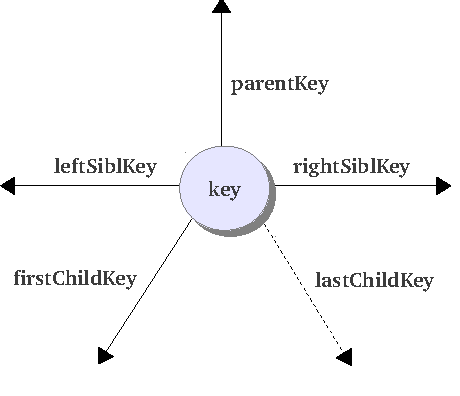
\includegraphics[width=0.45\textwidth]{figures/encoding}
%\caption{Treetank encoding} 
%\label{fig:encoding}
%\end{figure}

%\item[Page] The page-layer is motivated by ZFS \cite{ZFS}. It takes care of persisting nodes and is designed for the efficient storage of versioned tree-structures. The pages are stored in a rooted tree. A so called \emph{UberPage} contains indirect references (through references to \emph{IndirectPage}s which refer) to the stored \emph{RevisionRootPage}s. Based on the copy-on-write (COW) principle no data is lost with a minimum space consumption. Once a write transaction commits changes new \emph{NodePage}s containing modified nodes are persisted. NodePages which do not include changed nodes are not touched, therefore \emph{IndirectPage}s in subsequent revisions usually point to the same (persistent) data depending on the revisioning-strategy Treetank is configured to use.

%\item[I/O] The I/O layer is responsible for persisting and retrieving data. Currently a BerkeleyDB binding as well as a memory mapped File binding is available. A binding to Cloud Storage providers through \emph{JClouds} is in development.
%\end{description}

%The next section describes preliminaries and the implementation of the ID-less diff algorithm called FMSE, described in Chapter (\ref{sec::relwork}).

\subsection{ID-less diffing (FMSE) / Preprocessing}
Preprocessing of raw data is a major task in every data processing pipeline. Besides data specific preprocessing, databases/resources which do not evolve through the Java-API of Treetank have to be imported. Note that it is very common to simply dump full revisions of temporal data, thus most often no direct deltas are provided which just have to be applied to a base revision. Furthermore our prototype must be capable of comparing similar distinct trees. In both cases often times unique node-identifiers are not provided and therefore the trees or revisions thereof must be compared using tree-to-tree comparison heuristics which try to determine and match the most similar nodes/subtrees. %In subsequent steps unmatched nodes are either to edit unmatched nodes afterwards (insert/delete/move). Thus, to take full advantage of the decreased storage costs regarding revisioned data in Treetank as well as to use the subsequent ID-based difference-algorithm and the visualizations, first of all differences between the tree-structures have to be computed.

%As most tree-structures do not include unique node-identifiers a diff-algorithm which compares tree-structures based on predefined similarity measures,
As described in the introduction the Fast Matching Simple EditScript (FMSE) algorithm is implemented. The reasons for choosing FMSE are based on three properties: (1) it is successfully implemented a few times (specifically for XML-documents) \cite{xmldiff}, \cite{diffxml}, (2) it utilizes Treetank's cheap move-operation and (3) supports applying edit-operations/changes on the fly. Our implementation emerged from a rewrite of the DOM-implementation of Daniel Hottinger and Franziska Meyer described in \cite{diffxml}. The new move-operation which is supported by Treetank is defined on subtrees and very lightweight. Only local nodes (parent, siblings, first-child) are affected as well as the ancestor nodes of the node which moves (before and after the move). Ancestor nodes are only modified if hash-values are enabled which represent a fingerprint of the whole subtree and support a faster version of our ID-based diffing algorithm described in the next section. 

The Nodes are matched based on a bottom-up (postorder) traversal searching for the Longest Common Subsequence (LCS) of matching nodes. Predefined functions determine the similarity of nodes/subtrees as described in Chapter \ref{sec::relwork} which are utilized by the LCS-algorithm to determine matches. Unmatched nodes after determining the LCS are examined for crossmatches (moves). The algorithm not only facilitates the analysis of temporal evolving tree-structures but also the comparison of similar distinct trees. To support the FMSE implementation and expressive visualizations Treetank is enhanced in several ways. The following new operators/methods and components are available:

\begin{itemize}
\item \texttt{LevelOrderAxis} which incorporates attribute- and namespace-nodes if desired.
\item \texttt{copy-operation} to copy nodes/subtrees of other \emph{database/resource}-tuples.
\item \texttt{move-operation} to move nodes/subtrees in the currently opened \emph{resource}.
\item \texttt{replace-operation} to replace a node and its subtree with another node/subtree.
\item Visitor pattern support for nodes/transactions.
\item Merging or avoidance of adjacent text nodes at any time.
\end{itemize}

The \texttt{LevelOrderAxis} and the other operations are described in Appendix \ref{subsubsec::levelorderaxis} and \ref{subsec::operations}. The granularity of the operations are important:

\begin{itemize}
\item \texttt{insert}-operations are defined on leaf nodes. It is not possible to insert inner nodes, however this is only an implementation restriction and simplifies our identifier-based diffing algorithm. Due to the pointer-based encoding of Treetank, however it is possible to include an insert-operation to insert nodes between inner nodes in constant time. Currently, the only workaround is an insert followed by a move.
\item \texttt{remove}-operations always delete the whole subtree of the node to remove.
\item The \texttt{update}-operation is defined on inner- as well as on leaf-nodes and updates only a single node.
\item The \texttt{move}-operation is defined on inner- as well as on leaf-nodes and moves the whole subtree.
\item The \texttt{replace}-operation is defined on inner- as well as on leaf-nodes whereas the whole subtree of the node to replace is removed and thus replaced by the new node or subtree.
\item The \texttt{copy}-operation is defined on inner- as well as on leaf-nodes and also copies whole subtrees.
\end{itemize}

Having described the preliminaries the next section describes the FMSE implementation itself.

\subsubsection{FMSE} The FMSE implementation first saves node-types and the according node-IDs in two associative arrays during a postorder traversal. Next, the algorithm determines a longest common subsequence of matching nodes. Leaf nodes are compared first, then inner nodes. Thus the inorder-traversal described in \cite{chawathe1996change} must be replaced by a postorder-traversal. Otherwise, some leaf nodes required to determine the similarity of inner nodes are not processed beforehand. The matching of nodes involves two different similarity-metrics as described in the last chapter. However our implementation bears some explanation, as the matching is crucial and the changes applied by FMSE are propagated to a subsequent ID-based diffing-algorithm:

\begin{itemize}
\item \texttt{TextNode}s are matched based on their String-value. The Levenshtein algo\-rithm is used to compute a similarity measure of the values, which counts update costs of individual characters normalized between 0 and 1. \texttt{QName}s of \texttt{Namespace}- and \texttt{attribute}-nodes are matched first based on equality. In case of attributes afterwards their value is compared yet again using the Levenshtein algorithm in addition to their ancestor-elements.

\item \texttt{ElementNode}s are compared based on the number of matched nodes in their subtree. Thus not only leaf nodes are compared as suggested in the paper. Recapitulate that all node-types are chained for the fast\-Matching-algorithm bottom up during a postorder traversal. Empty elements however are compared based on their \texttt{QName} similarity, whereas all ancestor nodes are compared, too once more utilizing Levenshtein. This ensures the possibility of matching empty-elements after a deletion or insertion of a subtree. Treating empty nodes as leaf nodes otherwise prohibits matching empty \texttt{element}-nodes with other \texttt{element}-nodes which include a subtree because leaf nodes and internal nodes are compared in different successive steps and thus are not cross-compared. Matching nodes are stored in a \texttt{BiMap} containing forward and backward matchings of nodeKeys.
\end{itemize}

After storing matching node-IDs, FMSE step one is implemented straight forward. However whenever an \texttt{attribute}- or \texttt{namespace}-node is determined to be moved it is deleted from the old parent and inserted at the new parent node as moves of these node-types are not permitted by Treetank. Another noteworthy subject regarding moves is, that deleted text nodes in case adjacent nodes are collapsed and must be removed from the mapping as well. Due to adding the consistency constraint that \emph{never}, before and after a commit, duplicate attributes with the same \texttt{QName} are permitted, a new attribute value is set in the \texttt{WriteTransaction.insertAttribute(QName, String)} method instead of adding a new one if the \texttt{QName} of the attribute to insert is identical to another attribute-node with the same parent. This also saves from time overhead due to node-creation. This case occurs whenever the attributes with the same \texttt{QName} and parent node are not matched because of very different attribute-values or parent \texttt{QName}s. All updated or inserted nodes are added to the matches as described by Chawathe et al. in \cite{chawathe1996change} to prevent them from deletion in the next step.

The second FMSE step, which deletes non matching nodes with their whole subtrees, involves a preorder traversal of the tree. Thus a new \\\texttt{VisitorDescendantAxis} which optionally expects a visitor instance is implemented \footnote{Visitors are always preferable to other methods if algorithms depend on the specific node-types, due to runtime errors during downcasts or possibly long chains of \texttt{instanceof} checks} and detailed in Appendix \ref{subsec::visitor}. 

The following cases have to be distinguished. The node to move

\begin{enumerate}
\item has no right- and no left-sibling
\item has no right- and no left-sibling but the parent has a right-sibling (the parent must be removed from a stack which is used to save right-siblings for nodes which have a first child.)
\item has a right- and a left-sibling
\item has no right- but a left-sibling
\item has a right- but no left-sibling
\end{enumerate}

Two variants of the third case are depicted in Fig. \ref{fig:deletionvisitor}. In case the node to delete has two neighbour nodes which are \texttt{TextNode}s (node 4) the right sibling value is appended to the left \texttt{TextNode}. The right sibling node is removed from the storage afterwards, too. Next, the transaction is located at the updated left sibling text node. Thus the preorder traversal in the \texttt{VisitorDescendantAxis} continues without skipping any nodes. Otherwise if no adjacency text nodes are merged during the remove()-operation (node 9) the transaction is moved to the right-sibling before the operation is finished. Thus, the transaction first has to be moved to the left sibling before the \texttt{VisitorDescendantAxis} moves the cursor to the right-sibling. In this case the subtree of node 8 must be skipped as it is processed before.

\begin{figure}[tb]
\center{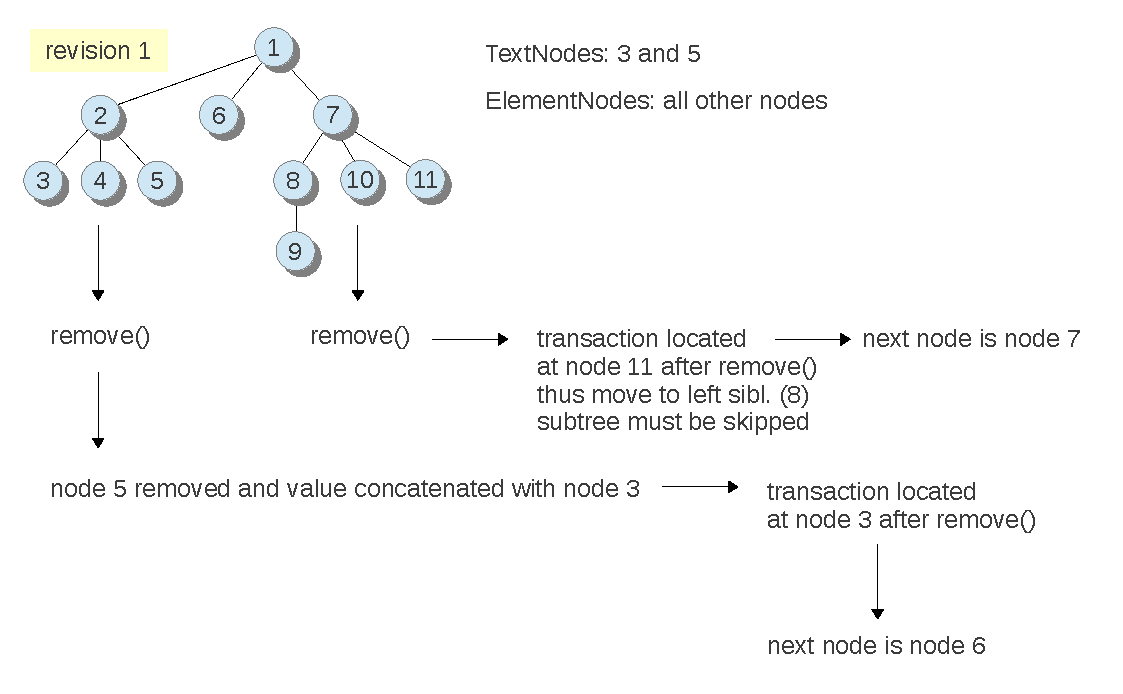
\includegraphics[width=\textwidth]
{figures/deletionvisitor}}
\caption{\label{fig:deletionvisitor} Deletion visitor; two variants are depicted for the case that the node to removed has a left- and a right-sibling. Either both sibling nodes are \texttt{TextNode}s as is the case for node 4 or not (node 10).}
\end{figure} 

\subsection{ID-based diffing}
Once revisioned data is stored in Treetank the main task is to reveal and present structural differences of the tree-structures. Treetank supports collections in form of databases which include one or more resources. Due to stable unique node IDs in each resource every kind of tree-structure is imported updating a single resource with the computed changes using FMSE. Even similar distinct tree-structures are imported updating a single resource. Otherwise, we would not be able to utilize unique node-IDs as different resources do not share unique node-IDs.

A fast linear time diff-algorithm utilizes these unqiue node-IDs and optionally hash-values which represent the content of the entire subtree rooted at a specific node. Note that the algorithm is designed to be able to compare any two revisions and thus not just consecutive revisions. It compares two nodes each time and determines the type of diff. 

%\begin{figure}[tb]
%\center{\includegraphics[width=\textwidth]
%{figures/diff}}
%\caption{\label{fig:diff} Two revisions of a tree-structure and the edit-operations involved. By comparing consecutive revisions the edit-operations usually equal the diff-types considering \texttt{REPLACEDOLD/REPLACEDNEW} as one operation just like \texttt{MOVEDFROM/MOVEDTO}.}
%\end{figure} 

\subsubsection{Hashes} One of our goals is the efficiency of our approach as it is called by our interactive visualizations described in the next chapter. Hashes of all nodes are generated during import in a postorder-traversal and an ancestor-traversal if subtrees are inserted. A new bulk insertion mode in Treetank speeds up the import and reduces the asymptotic bound from $O(n^2+m)$ to $O(n+m)$ whereas $n$ is the number of nodes to import and $m$ is the number of ancestor nodes for which the hash-values have to be adapted. They are build incrementally based on all nodes in a subtree bottom up. Two types of hashes are available, rolling\cite{Rolling2011}- and postorder\cite{Integrity2010}- hashes. \emph{Rolling} hashes only affect the inserted or updated nodes on the ancestor axis whereas \emph{postorder} hashes also affect nodes in a postorder traversal starting at the current node. The hashes are optionally used to speed up our algorithm. Whenever identical hashes are determined the nodes are matched and the two transactions opened on the two revisions and used to iterate over both revisions are moved to the next node in document order, which is not a descendant of the current node. Thus the transactions move to the first node in the XPath \texttt{following::}-axis. Hence, whole subtrees are skipped from traversal. The hashes include the unique node-IDs as well as node specific content. The hashing-function is designed to be fast and to reduce collisions to a minimum. Even if hash-collisions which are extremely unlikely appear it is not possible to match subtrees with identical hash-values as the node-IDs are also compared which are stable and unique during all revisions. Rolling-hashes are enabled by default during the database/resource creation and optionally used by our diff-algorithm. It is for instance used by an optional pruning of the tree in a Sunburst-layout to speed up the computation as well as the construction of the visualization. An in depth explanation of this application is provided in Chapter \ref{sec::visualizations}. The next subsection briefly describes two modes of the algorithm.

\subsubsection{Modes to compare differences} Interested observers are notified of the diff between two nodes through registration and the implementation of a special interface method. Currently two modes are available.

\begin{itemize}
\item \emph{Structural Diff} calculates changes without comparing attribute and namespace nodes. This implies that whenever the overall structure is crucial this algorithm should be chosen.
\item \emph{Full Diff} takes structural nodes as well as attribute and namespace nodes into account. However currently we do not emit non-structural changes. Changes in \texttt{namespace}- or \texttt{attribute}-nodes result in an \texttt{UPDATED} parent-element. This restriction applies as the \emph{SunburstView} which is described in Chapter \ref{sec::visualizations} currently does not include special \texttt{namespace}- or \texttt{attribute}-items. Instead these are part of the element item and shown on mouseover.
\end{itemize}

The following diff-types are supported and emmited:

\begin{itemize}
\item \texttt{INSERTED} denotes that a node is inserted.
\item \texttt{DELETED} denotes that a node is removed.
\item \texttt{UPDATED} denotes that a node is updated, that is either the QName of an \texttt{element}-node is updated or the value of a \texttt{text}-node.
\item \texttt{SAME} denotes that a node is not changed.
\item \texttt{REPLACEDOLD} denotes that a node or subtree is replaced (the old node/subtree).
\item \texttt{REPLACEDNEW} denotes that a node or subtree is replaced (the new node/subtree).
\item \texttt{SAMEHASH} denotes that a node is not changed and the hashes of the subtrees are identical.
\end{itemize}

Note that the differentiation between \texttt{REPLACEDOLD/REPLACEDNEW} supports an expressive aggregated tree-structure used as an underlying model of the visualizations. However it is only a simple heuristic. Two other diff-types are supported by an optional post-processing step.

\begin{itemize}
\item \texttt{MOVEDFROM} denotes that a node or whole subtree has been moved from this location to another one.
\item \texttt{MOVEDTO} denotes that a node or whole subtree has been moved to this location.
\end{itemize}

The types are splitted, too to indicate the movement of the node, the old place before the move and the new place in the aggregated tree-structure.

The next section describes the preorder-traversal in both revisions which is essential to compare the right nodes each time.

\subsection{Traversal of both revisions}
The algorithm to traverse the trees and to compute the differences between two nodes in each revision is depicted in algorithm \ref{overallDiffAlgo}. First, the method\\ \texttt{treeDeletedOrInserted(IReadTransaction, IReadTransaction)} checks if\\ both transactions opened on each revision can be moved to the start node. If not, either the node is inserted or deleted depending on the transaction which can not be moved.

Let's examine both cases:
\begin{itemize}
\item
The transaction opened on the older revision can not be moved to the start node. This implies that the tree in the new revision has been inserted.
\item
The transaction opened on the newer revision can not be moved to the start node. This implies that all nodes in the old transaction have been deleted.
\end{itemize}

The distinction is used to support the selection of modified nodes in the visualizations which are described in Chapter \ref{sec::visualizations} and only affects subtrees. Otherwise simply put all nodes in the old revision are deleted, whereas all nodes in the new revision are inserted.

If the root-nodes of both revisions are selected by the transactions they move forward in \emph{document order} (depicted in Fig. \ref{fig:id-diff}) depending on the last encountered kind of diff between two nodes. Document order is identical to a preorder traversal of a tree. In case of an insert, the transaction opened on the new revision is moved forward, in case a delete is encountered the transaction opened on the old revision is moved forward (the \\ \texttt{moveCursor(IReadTransaction, ERevision)}-method). In both cases the whole subtree is emitted (for instance node 10 and its subtree in Fig. \ref{fig:id-diff} is deleted). If a node is updated or is not changed at all both transactions move to the next node in document order. Once the traversal in one of the two revisions reaches the end of the tree, the transaction is located at the document root. The diff-calculation ends if either the transaction on the older revision is located at the document root and the last encountered type of diff was \texttt{DELETED} or both transactions are located at their document-root nodes. Note that if the transaction on the newer revision is located at the document root, but the transaction on the old revision is not the following nodes are \texttt{DELETED} at the end of the tree and have to be emitted as such (lines 22-28; node 15 in Fig. \ref{fig:id-diff}). 

\begin{figure}[tb]
\center{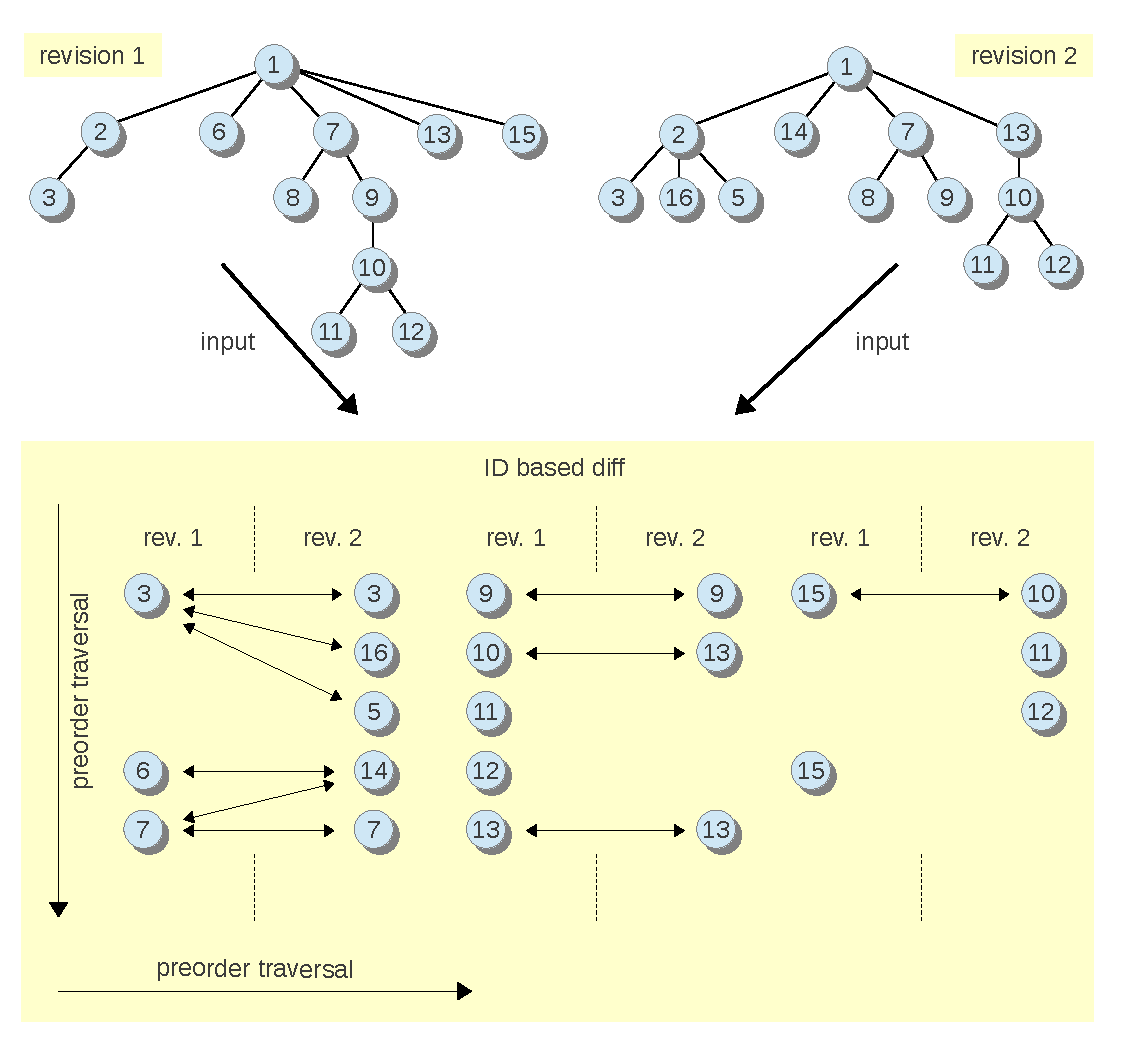
\includegraphics[width=\textwidth]
{figures/id-diff}}
\caption{\label{fig:id-diff} ID-based diffing.}
\end{figure} 

\begin{algorithm}[Hhtbp]
\SetKwInOut{Input}{input}\SetKwInOut{Output}{output}
\Input{HashKind mHashKind, long pOldRevKey, long pNewRevKey, long mOldStartKey, long mNewStartKey, DiffType pDiffType, DiffTypeOptimized mDiffKind, ISession mSession}
\Output{for each node comparsion: DiffType diffType, IStructNode oldNode, IStructNode newNode, Depth depth}
\BlankLine
INodeReadTransaction rtxOld $\leftarrow$ mSession.beginNodeReadTransaction(pOldRevKey)\;
INodeReadTransaction rtxNew $\leftarrow$ mSession.beginNodeReadTransaction(pNewRevKey)\;
\tcp{moveTo(long) returns true in case the transaction could be moved to the node or false otherwise.}
newRtxMoved $\leftarrow$ rtxNew.moveTo(mNewStartKey)\;
oldRtxMoved $\leftarrow$ rtxOld.moveTo(mOldStartKey)\;

treeDeletedOrInserted(newRtxMoved, oldRtxMoved)\;

DiffType $\leftarrow$ null\;
\tcp{Check first node.}
\If{mHashKind == HashKind.None OR mDiffKind == DiffTypeOptimized.NO}{
  diff $\leftarrow$ diff(rtxNew, rtxOld, depth)\;
}\Else{
  diff $\leftarrow$ optimizedDiff(rtxNew, rtxOld, depth)\;
}

\tcp{Iterate over new revision (order of operators significant -- regarding the OR).}
\If{diff != DiffType.SAMEHASH}{
  \While{(rtxOld.getNode().getKind() != ENode.ROOT\_KIND AND diff == DiffType.DELETED) OR moveCursor(rtxNew, ERevision.NEW)}{
  \If{diff != DiffType.INSERTED}{
    moveCursor(rtxOld, ERevision.OLD)\;
  }

  \If{rtxNew.getNode().getKind() != ENode.ROOT\_KIND
   or rtxOld.getNode().getKind() != ENode.ROOT\_KIND}{
    \If{mHashKind == HashKind.None OR mDiffKind == DiffTypeOptimized.NO}{
      diff $\leftarrow$ diff(rtxNew, rtxOld, depth)\;
    }\Else{
      diff $\leftarrow$ optimizedDiff(rtxNew, rtxOld, depth)\;
    }
  }
}

\tcp{Nodes deleted in old rev at the end of the tree.}
\If{rtxOld.getNode().getKind() != ENode.ROOT\_KIND}{
  emitOldNodes(rtxNew, rtxOld, depth)\;
}
}

done()\;
\caption{ID-based diff: traversal}\label{overallDiffAlgo}
\end{algorithm}

\subsection{Diff-Computation}
Besides moving both transactions forward in document-order depending on the last encountered type of diff the algorithm which determines the type of difference itself is crucial. The computation is the main task of the \\ \texttt{diff(INodeReadTransaction, INodeReadTransaction, Depth)}-method outlined in algorithm \ref{diffAlgo}. It is invoked whenever the node-IDs or the \texttt{QName}s/\texttt{Text}-values of the nodes to compare differ.

\begin{algorithm}[Hhtbp]
\SetKwInOut{Input}{input}\SetKwInOut{Output}{output}
\Input{Depth pDepth, INodeReadTrx pOldRtx, INodeReadTrx pNewRtx}
\Output{kind of diff (DiffType enum value)}
\BlankLine
DiffType diff $\leftarrow$ DiffType.SAME;

\tcp{Check if node has been deleted.}
\If{pDepth.getOldDepth() $>$ pDepth.getNewDepth())}{ 
  diff $\leftarrow$ DiffType.DELETED\;
  cumulatDiffTypes(diff)\;
  \If{checkReplace(pNewRtx, pOldRtx)}{
    diff $\leftarrow$ DiffType.REPLACED\;
  }
}\tcp{Check if node has been updated.}\ElseIf{checkUpdate(pNewRtx, pOldRtx)}{ 
  diff $\leftarrow$ DiffType.UPDATED\;
}\tcp{Check if node has been replaced.}\ElseIf{checkReplace(pNewRtx, pOldRtx)}{ 
  diff $\leftarrow$ DiffType.REPLACED\;
}\Else{
  long oldKey $\leftarrow$ pOldRtx.getNode().getNodeKey()\;
  boolean movedOld $\leftarrow$ pOldRtx.moveTo(pNewRtx.getNode().getNodeKey())\;
  pOldRtx.moveTo(oldKey);

  long newKey $\leftarrow$ pNewRtx.getNode().getNodeKey()\;
  boolean movedNew $\leftarrow$ pNewRtx.moveTo(pOldRtx.getNode().getNodeKey())\;
  pNewRtx.moveTo(newKey);

  \If{!movedOld}{
    diff $\leftarrow$ DiffType.INSERTED\;
  }\ElseIf{!movedNew}{
    diff $\leftarrow$ DiffType.DELETED\;
  }\Else{
    \tcp{Determine if one of the right sibling matches.}
    EFoundEqualNode found $\leftarrow$ EFoundEqualNode.FALSE\;
    long key $\leftarrow$ pOldRtx.getNode().getNodeKey()\;

    \While{pOldRtx.getStructuralNode().hasRightSibling() AND pOldRtx.moveToRightSibling()
      AND found == EFoundEqualNode.FALSE}{
      \If{checkNodes(pNewRtx, pOldRtx)}{
        found $\leftarrow$ EFoundEqualNode.TRUE\;
        break\;
      }
    }

    pOldRtx.moveTo(key)\;
    diff $\leftarrow$ found.kindOfDiff()\;
  }

  cumulatDiffTypes(diff)\;
}

return diff\;
\caption{ID-based diff: diff-computation}\label{diffAlgo}
\end{algorithm}

First, the depths of the nodes have to be compared. The depth is the sum of nodes in the path up to the root-node. When the depth of the node in the old revision is greater than the depth of the node in the new revision it must have been deleted. Note that the depths are not persisted, thus counters have to keep track of the current depths. All diff-tuples which are of type \texttt{DiffType.DELETED} or \texttt{DiffType.INSERTED} are saved in a Java \texttt{List}. A second datastructure is used to gather the diff types itself, that is a whole subtree which is either inserted or deleted is cumulated by the according diff-type. This datastructure is used to find \texttt{INSERTED}, \texttt{DELETED} combinations which are instead emitted as of type \texttt{DiffType.REPLACEDOLD} (the deleted tuples) and \texttt{DiffType.REPLACENEW} (the inserted tuples).

When the depth of the node in the old- and the node in the new-revision instead either is identical or the depth of the node in the more recent revision is greater it is checked whether the node is updated through comparison of the node-IDs and the depths/levels of the nodes. Unless the node is updated the node is examined for replacement. Therefore the datastructure which keeps track of deleted- and inserted-subtrees is reviewed. Consecutive insert/delete- or insert/insert/delete/delete-tuples are emitted as replaced subtrees. Note that this replace-detection is just a simple heuristic and currently does only detect the aforemeantioned pairs of inserted and deleted nodes.%The datastructure in either case is emptied even if no matching types are found. Furthermore when two diff-types previously have been stored in the datastructure the \texttt{List} of diff-tuples must immediately be emitted in case a replace has been detected and the datastructure must be reinitialized \footnote{for instance replaced with a new instance} afterwards. Four elements are always immediately emitted regardless of whether the diff-types have changed or not. In the first case subsequently the replaced tuples must be emitted.

Assuming a node or subtree is not replaced, it must be decided if either the current node in the new revision is inserted or the current node in the old revision is deleted. First, it is determined if the transaction opened on the old revision is moveable to the current node in the new revision. If not it is immediately obvious that the node is inserted. Otherwise, if the transaction opended on the new revision can \emph{not} be moved to the current node in the old revision it must be a deleted node. For the simple reason that move-operations are supported both checks might succeed. In this case the right siblings of the node in the old revision have to be examined in order to determine the type of diff, until one of them matches the node in the new revision, that is the node-IDs are identical or no more right siblings are available. In the first case the new node is inserted. Otherwise it is deleted.

\subsection{Detecting moves}
An optional postprocessing step is required to detect moves. The two basic diff-types \texttt{MOVEDFROM} and \texttt{MOVEDTO} are detected after all operations are emitted. The detection requires three datastructures to store all diff-types, the inserted nodes and the deleted nodes.

\subsubsection{Impossibility to detect moves on the fly} Note that it is not possible to include the detection of moves in the preorder-traversal of both revisions itself, as it is not known in advance which of the two nodes is the one which is moved and which one is the node which is unchanged. However this is required to determine which of the two transactions must be moved to the next node in document order. All we can argue is, that it is possible to detect a move itself if the transaction on the new revision is moveable to the current node of the transaction in the old revision and vice versa. That is all \texttt{DELETED} or \texttt{INSERTED} nodes have already been emitted, meaning that one of the two nodes which are currently compared must have been moved and the other must have been unchanged. It is not possible to decide which one of the two nodes stayed the same and which one has been moved. The position in the tree is no implication wheter a node has been moved from or moved to another place, but this is crucial to decide which of the two nodes has not changed and which one actually has been moved. As thus the types have to be matched. Whenever the unique nodeKey of a \texttt{DELETED}-node matches the key of an \texttt{INSERTED}-node, the corresponding diff-types can be changed into \texttt{MOVEDFROM} and \texttt{MOVEDTO}. The next subsection details a postprocessing algorithm which is based on this idea.

\begin{algorithm}[tb]
\SetKwInOut{Input}{input}\SetKwInOut{Output}{output}
\Input{Map allDiffs, Map inserted, Map deleted}
\Output{none (void)}
\BlankLine
\tcp{For every diff tuple in the map which saves all encountered diffs in document-order}
\For{Diff diffTuple : allDiffs.values()}{
  Integer newIndex $\leftarrow$ inserted.get(diffTuple.getOldNodeKey())\;
  \If{newIndex != null
    AND (diffTuple.getDiff() == DiffType.DELETED OR diffTuple.getDiff() == DiffType.MOVEDFROM)}{
      allDiffs.get(newIndex).setDiff(DiffType.MOVEDTO)\;
  }
  Integer oldIndex $\leftarrow$ deleted.get(diffCont.getNewNodeKey())\;
  \If{oldIndex != null
    AND (diffTuple.getDiff() == DiffType.INSERTED OR diffTuple.getDiff() == DiffType.MOVEDPASTE)}{
      allDiffs.get(oldIndex).setDiff(DiffType.MOVEDFROM).setIndex(
                 inserted.get(diffTuple.getNewNodeKey()))\;
  }
}
\caption{ID-based diff: postprocessing to detect moves}\label{diffPostprocessing}
\end{algorithm}

\subsubsection{Detection of moves in a postprocessing step} All encountered diff-types are saved in an associative array, a map (index of their encounter $\Leftrightarrow$ diff-tuple) \footnote{which is used just like a List, to switch between a map implementation based on a persistent BerkeleyDB database depending on a specified threshold value or a simple LinkedHashMap instance} in preorder which is the order in which they are observed. Additionally \texttt{DELETED} and \texttt{INSERTED} nodes are recorded mapping their unique node-ID to the index in the original map with all entries. The algorithm described in \ref{diffPostprocessing} expects the three maps. It tries to match \texttt{INSERTED} $\Leftrightarrow$ \texttt{DELETED} pairs and vice versa and checks whether the diffType in the map needs to be adjusted to \texttt{MOVEDTO} or \texttt{MOVEDFROM} (or not at all). A map which does not contain a value for the specified key returns the special value \texttt{null}. First, the old node-ID (might have been deleted) is searched for in the Map containing all inserted tuples. If the key is found (value $!=$ null) the type is checked. If the current diff-tuple is of type \texttt{DELETED} or \texttt{MOVEDFROM} the diff type is set to \texttt{MOVEDTO}. Note that the check for the \texttt{MOVEDFROM} type is necessary as the corresponding \texttt{INSERTED} tuple might have been encountered before and thus the type has been changed to \texttt{MOVEDFROM} already. The following is the inverse case to set the \texttt{MOVEDFROM} type if necessary. Furthermore a link in the form of the index of the matching node with the same node-ID and the corresponding \texttt{MOVEDTO} diff-type is additionaly saved. Note that the algorithm does not detect \texttt{text}-nodes which are moved to a right sibling of another \texttt{text}-node. In this case our implementation of the \texttt{moveSubtreeToRightSibling(long)} prepends the value of the current \texttt{text}-node to the moved \texttt{text}-node and subsequently deletes the current node. This ensures, that no two text-nodes are ever adjacent which otherwise contradicts the XQuery/XPath data model (XDM). In this particular edge case the algorithm determines a \texttt{REPLACED} node (a direct consequent from the deletion of the node the transaction resides at and the insertion of the moved node with the prepended text-value) and a \texttt{DELETED} node (the node which has been moved).

\subsection{Runtime/Space analysis and scalability of the ID-based diffing algorithm}
The runtime of the ID-based diff algorithm is $O(n+m)$ whereas $n$ is the number of nodes in the first tree and $m$ the number of nodes in the second tree. It is thus a fast linear diff-computation in comparison to the FMSE-algorithm ($O(n*e+e^2)$, $n$ is the number of unchanged nodes and $e$ the number of changed nodes) which is used in the first place to determine the differences which are imported. The space-consumption is $O(1)$ and in case the replace-operation is enabled at worst $O(k)$. $k$ is the sum of the subtrees which are cached (at most 4 subtrees currently). However the space consumption of an aggregated tree-structure which is going to be described in the next chapter (\ref{sec::visualizations}) is $O((u+v)*k)$. $u$ is the number of unchanged nodes, $v$ is the number of changed nodes and $k$ is tuple relevant stuff (type of diff, the nodes and the depths in both trees). Thus the asymptotic space consumption is linear depending only on the number of unchanged and changed nodes.

Our performance evaluation involves measuring the scaling during random modification-patterns (Fig. \ref{fig:100MBscaling}) and different document sizes with scaled modi\-fication-patterns (Fig. \ref{fig:docScaling}). The modification-patterns are increased in the same scale as the document size such that the documents are modified with approximately the same number of modifications. The hardware used is a common notebook with 4Gb RAM and a Core 2 Duo 2,66 Ghz CPU. All performance-measures are executed 20 times. Fig. \ref{fig:100MBscaling} shows that the number of modifications minimally affects the runtime. The runtime decreases linear as less modifications between two revisions are encountered. However the linear decrease is minimal due to a few more value and node-ID comparisons.

Fig. \ref{fig:docScaling} (Table \ref{chap3:compDiffInstances}) depicts the scaling during different document sizes and modification schemes. The scale is logarithmic, thus we are able to identify the linear runtime due to increased document sizes. It therefore emphasizes the asymptotic bound.

\begin{figure}[tb]
\centering
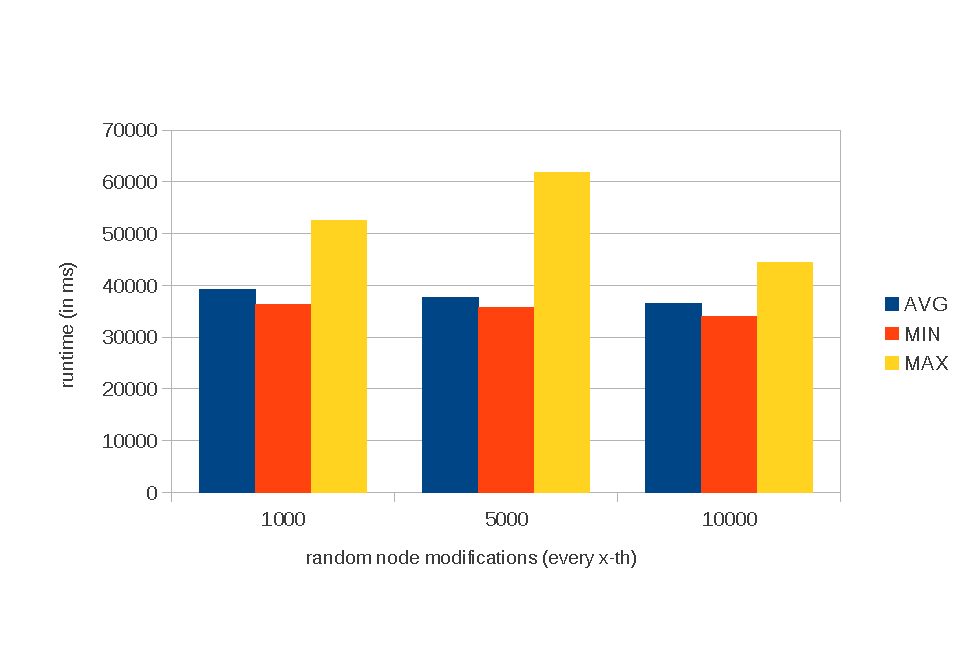
\includegraphics[width=\textwidth]{figures/100MB-scaling}
\caption{Scaling during different modification-patterns (update/insert/delete/replace/move every 1000st, 5000st and 10000st node) in a 111 MiB XMark instance.} 
\label{fig:100MBscaling}
\end{figure}

\begin{table}[tb]
\centering 
\begin{tabular}[r]{|l|c|c|c|c|c|} 
\hline
\textbf{modifications} & \textbf{min} & \textbf{max} & \textbf{average} & \textbf{stddef} & \textbf{conf95}\\
\hline
\hline
\textbf{1000} & 36265.14 & 52459.38 & 39167.75 & 4416.66 & [36270.63-52288.26]\\
\hline
\textbf{5000} & 35717.34 & 61860.29 & 37650.67 & 5776.44 & [35717.67-60728.71]\\
\hline
\textbf{10000} & 33948.96 & 44451.06 & 36579.37 & 2805.09 & [33979.75-44336.83]\\
\hline
\end{tabular}
\label{chap3:comparsion}
\vspace{0.5em} 
\caption{Comparsion of different modification-patterns of a 111 MiB XMark instance (update/insert/delete/replace/move every 1000st, 5000st and 10000st node). Runtime in ms.}
\end{table}

%\begin{table}[tb]
%\centering 
%\begin{tabular}[r]{|l|c|c|c|} 
%\hline
%modifications & \textbf{1000} & \textbf{5000} & \textbf{10000}\\
%\hline
%\hline
%\textbf{min} & 36265.14 & 35717.34 & 33948.96\\
%\hline
%\textbf{max} & 52459.38 & 61860.29 & 44451.06\\
%\hline
%\textbf{av} & 39167.75 & 37650.67 & 36579.37\\
%\hline
%\end{tabular}
%\label{chap3:comparsion}
%\vspace{0.5em} 
%\caption{Comparsion of different modification-patterns of a 111 MiB XMark instance (update/insert/delete/replace/move every 1000st, 5000st and 10000st node). Runtime in ms.}
%\end{table}

\begin{figure}[tb]
\centering
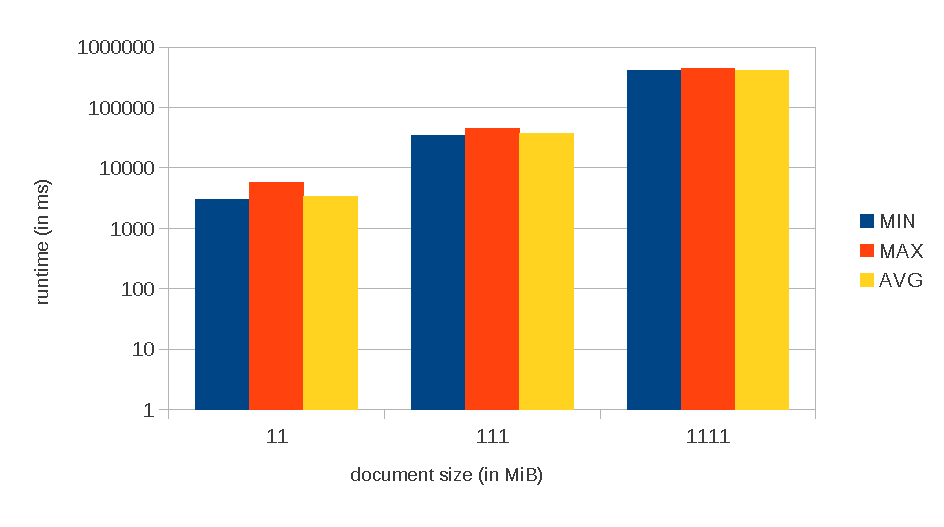
\includegraphics[width=\textwidth]{figures/diff-docsize-scale}
\caption{Different document sizes with modification-count scaled accordingly (11 MiB $\Leftrightarrow$ modifiy every 1000th node, 111 MiB $\Leftrightarrow$ modify every 10000 th node, 1111 MiB $\Leftrightarrow$ modify every 100000th node / Y-axis logarithmic scaled.)} 
\label{fig:docScaling}
\end{figure}

\begin{table}[tb]
\centering 
\begin{tabular}[r]{|l|c|c|c|c|c|} 
\hline
\textbf{document size} & \textbf{min} & \textbf{max} & \textbf{average} & \textbf{stddef} & \textbf{conf95}\\
\hline
\hline
\textbf{11 MiB} & 2957.79 & 5694.65 & 3323.96 & 627.11 & [2958.82-5610.53]\\
\hline
\textbf{111 MiB} & 33948.96 & 44451.06 & 36579.37 & 2805.09 & [33979.75-44336.83]\\
\hline
\textbf{1111 MiB} & 401878.64 & 439337.71 & 413158.13 & 11211.11 & [401904.84-439033.71]\\
\hline
\end{tabular}
\label{chap3:compDiffInstances}
\vspace{0.5em} 
\caption{Comparsion of different XMark instances (11 MiB, 111 MiB, 1111 MiB modifying every 1000st, 10000st and 100000st node). Runtime in ms.}
\end{table}

%\begin{table}[tb]
%\centering 
%\begin{tabular}[r]{|l|c|c|c|} 
%\hline
%& \textbf{11 MiB} & \textbf{111 MiB} & \textbf{1111 MiB}\\
%\hline
%\hline
%\textbf{min} & 2957.79 & 33948.96 & 401878.64\\
%\hline
%\textbf{max} & 5694.65 & 44451.06 & 439337.71\\
%\hline
%\textbf{average} & 3323.96 & 36579.37 & 413158.13\\
%\hline
%\end{tabular}
%\label{chap3:compDiffInstances}
%\vspace{0.5em} 
%\caption{Comparsion of different XMark instances (11 MiB, 111 MiB, 1111 MiB modifying every 1000st, 11000st and 122221st node). Runtime in ms.}
%\end{table}

Table \ref{chap3:compPrunedDiffInstances} shows the comparison based on the same documents as in Table \ref{chap3:compDiffInstances} however this time utilizing the hashes to skip the traversal of unchanged subtrees (nodes with identical hash-values and node-IDs). The runtime approximately halves in this example. It is obvious that the gain in speed depends on the subtree-sizes to skip. The worst case are modifications at leaf nodes in large, deep subtrees. In this case the hash-based optimization does not gain any speedup (in the 11 MiB XMark document with all leaf nodes updated approximately 4062.52ms in the average case compared to 4064.96ms for the hash-based optimization after 20 runs). In the best case modifications occur near the root node of large, deep subtrees (in the 11 MiB XMark document with depth 2 updated the runtime drops from 31979.92ms to 12280.01ms in the averge case). However, the XMark synthetic documents are not very deep, such that usually only a few nodes are skipped for every identical hash-value.

\begin{figure}[tb]
\centering
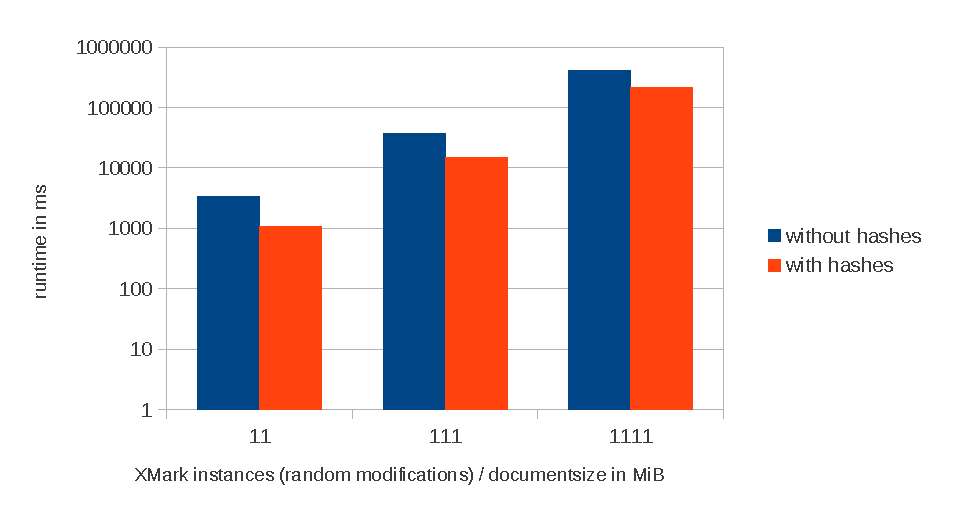
\includegraphics[width=\textwidth]{figures/diff-docsize-scale-pruned}
\caption{Different document sizes with modification-count scaled accordingly (11 MiB $\Leftrightarrow$ modifiy every 1000th node, 111 MiB $\Leftrightarrow$ modify every 10000th node, 1111 MiB $\Leftrightarrow$ modify every 100000th node. Y-axis logarithmic scaled)} 
\label{fig:docScaling}
\end{figure}

\begin{table}[tb]
\centering 
\begin{tabular}[r]{|l|c|c|c|c|c|} 
\hline
\textbf{document size} & \textbf{min} & \textbf{max} & \textbf{average} & \textbf{stddef} & \textbf{conf95}\\
\hline
\hline
%\textbf{11 MiB} & 1239.01 & 3698.94 & 1408.74 & 627.11 & [2958.82-5610.53] \\
\textbf{11 MiB} & 829.15 & 3943.55 & 1071.34 & 685.99 & [830.16-3809.75] \\
\hline
\textbf{111 MiB} & 14208.30 & 19135.01 & 14596.86 & 1073.83 & [14208.37-18912.52]\\
\hline
\textbf{1111 MiB} & 197223.12  & 271794.82 & 210296.70 & 17982.22 & [197235.36-269674.19]\\
\hline
\end{tabular}
\label{chap3:compPrunedDiffInstances}
\vspace{0.5em} 
\caption{Comparsion of different XMark instances skipping subtrees of nodes with identical hash-values (11 MiB, 111 MiB, 1111 MiB modifying every 1000st, 10000st and 100000st node). Runtime in ms.}
\end{table}

%\begin{table}[tb]
%\centering 
%\begin{tabular}[r]{|l|c|c|c|} 
%\hline
%& \textbf{11 MiB} & \textbf{111 MiB} & \textbf{1111 MiB}\\
%\hline
%\hline
%\textbf{min} & 1239.01 & 14208.30 & 197223.12\\
%\hline
%\textbf{max} & 3698.94 & 19135.01 & 271794.82\\
%\hline
%\textbf{average} & 1408.74 & 14596.86 & 210296.70\\
%\hline
%\end{tabular}
%\label{chap3:compPrunedDiffInstances}
%\vspace{0.5em} 
%\caption{Comparsion of different XMark instances skipping subtrees of nodes with identical hash-values (11 MiB, 111 MiB, 1111 MiB modifying every 1000st, 11000st and 111000st node). Runtime in ms.}
%\end{table}

The high max-runtime values are likely to be caused by the JVM warmup during the first or first few runs. This is also confirmed by invoking our Benchmarking Framework Perfidix with repeated invocations of only one run whereas the first invocation always yields the highest runtime by magnitudes. We furthermore encountered a very small linear decrease during the first few runs until a threshold value is reached likely due to filesystem caches.

\subsection{Conclusion and Summary}
We motivated the import of differences in Treetank between full dumps of temporal tree-structures or different similar trees to subsequently take full advantage of Treetanks' (1) revisioning strategies, (2) unique node-IDs which identify a node through all revisions and (3) hashes of each node, which almost guarantee a unique hash guarding the whole subtree through cryptographic rolling hashes. We implemented the FMSE-algorithm to support the initial import of differences of revisioned data (currently) in the form of XML-documents whereas each document represents one revision, a snapshot at a specific time. Considering no such data is available other even more sophisticated preprocessing steps have to be implemented before the FMSE-algorithm on the revisioned data in Treetank is useable. Two of the use cases which are going to be discussed in Chapter \ref{sec::applications} require further preprocessing. Note that the FMSE-algorithm does not require unique node-IDs and matches nodes based on a longest common subsequence (LCSS)-computation (which is ambiguous) on leaf- and inner-nodes in a bottom up traversal. Thus it might mismatchs similar nodes eventuating in too many edit-operations and thus only guarantees a minimum edit-script if the leaf node comparison-function is able to match exactly one corresponding node each time. The algorithm is particularly useful to compare similar different tree-structures which do not temporally evolve and usually naturally do not include node-IDs.

Furthermore we implemented many edit-operations which were not available in Treetank to support the implementation of the FMSE-algorithm and an expressive agglomerated tree-structure. We have shown that a subsequent diff-calculation based on IDs and hashes which guard the whole subtree usually is faster than the same algorithm without utilizing hashes. However it depends on the properties of the tree-structures and the modification patterns. Whenever large subtrees are unchanged, thus the subtree-roots have identical hash-values the runtime is reduced drastically.

Besides using hashes optionally to skip whole unchanged subtrees our ID-based diff-algorithm combines \texttt{INSERT/DELETE} and \texttt{INSERT/INSERT/DELETE/\\DELETE} sequences of whole subtrees to a single replace-operation. However it is only a simple heuristic.

Moves are optionally detected in a postprocessing-step by searching for \\\texttt{INSERT/DELETE} and \texttt{DELETE/INSERT} combinations with the same node-IDs. Move detection is especially useful to support analysts with an expressive visualization. Otherwise, especially in document-centric XML, for instance DocBook\cite{docbook} documents, it might be impossible to draw conclusions from simple inserts/deletes, whereas an author simply moved a sentence which is obscured due to other inserts/deletions of text and/or markup.

\cleardoublepage
\section{Visualizations}\label{sec::visualizations}
\subsection{Introduction}
The last chapter introduced the first part of the pipeline, the diff-algorithms in detail. Usually however sophisticated preprocessing-methods are needed, which are explained for a few applications in chapter \ref{sec::applications}.

This chapter describes several visualizations which help analysts to gain fast knowledge. First the GUI-framework which embeds various visualizations is briefly described. Next, an aggregation of the two tree-structures to compare follows.  the visualizations themselves are detailed. Our visualizations rely on the diff-algorithms described in Chapter \ref{sec::differences} and therefore depict the tree-edit distance, that is structural (insert/delete/move/replace) and non-structural (update) operations which transform one tree-structure into the other one. Different similarity measures are used to indicate the similarity of leaf-nodes and internal nodes either based on values or in the latter case based on overlapping subtree-structures. However the usage of similarity measures is highly modular and can be extended with further measures which either can be switched by user interaction or through heuristics. After briefly describing the \emph{TreeView} and the \emph{TextView} as well as basics of our specialized Sunburst layout, an explanation of filtering techniques follows which together with the ID-based diff-algorithm \footnote{usually the hash-based version comparing the hash-values of the nodes first} facilitates the analysis of even large tree-structures ranging from about 100MB to even GBs of data. The key assumption underlying this efficient diff-algorithm/visualization is that similar trees are compared and therefore only a small fraction of a tree-structure has to be transformed to derive the other tree-sturcture. Querying capabilities, similarity measures and the the visualization of moves are described subsequently. Next, Smallmultiple variants are detailed which facilitate the comparison of several tree-structures. The chapter concludes with a summary.

\subsection{GUI}
First, a GUI framework has been developed which incorporates several views. The framework has been written from scratch based on some key-ideas and software patterns used by BaseX \cite{BASEX}. The GUI is designed to be easily extendable. It currently offers the ability to view and interact with the stored Treetank data in many ways. Incorporated are several different views. Most of them are developed to support the analysis of differences as well as similarities between tree-structures. Others will be extended in the future. Furthermore the views are synchronized meaning that several types of actions in one view are reflected in other views as well. Special care is taken to adhere to the Model View Controller (MVC) architecture with a controller managing the interactions between the views which is depicted in Fig. \ref{fig:mvc}. The next section describes the visualizations in detail.

\begin{figure}[tb]
\center{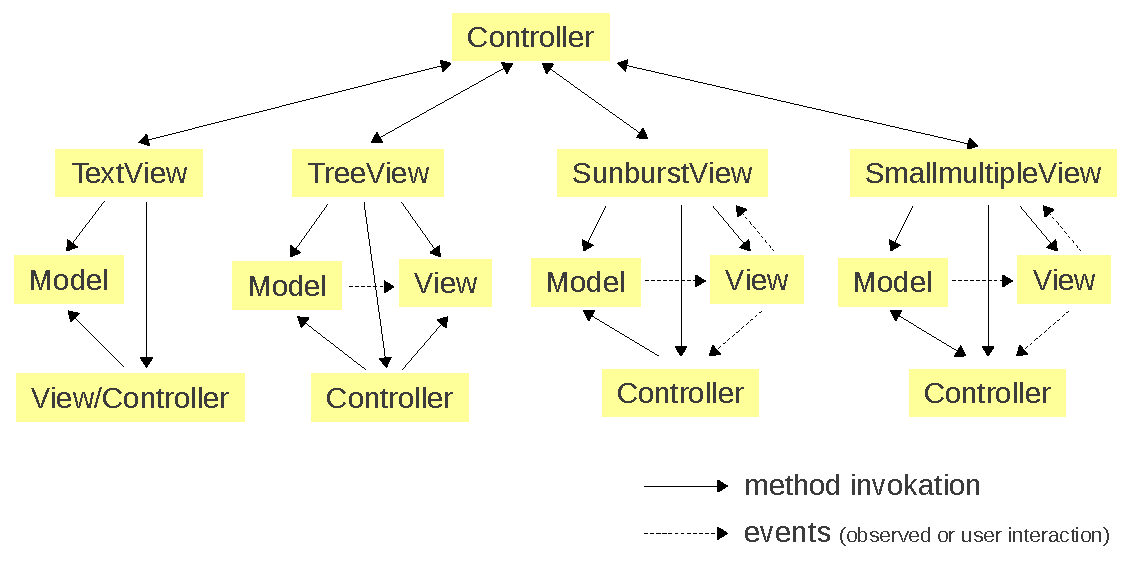
\includegraphics[width=\textwidth]
{figures/mvc}}
\caption{\label{fig:mvc} MVC-paradigm use. The \emph{TextView} and the \emph{TreeView} use standard Swing components. A \texttt{JTree} Swing-component is used implement the tree-model in the \emph{TreeView}. A \texttt{JTreeCellRenderer} implements the view and controller. It is responsible to translate user actions and to render the cells appropriately. The \texttt{JTextEditPane}-Swing component represents both the view and controller in the \emph{TextView} whereas a new \texttt{StAXDiffSerializer} described later on implements the \texttt{XMLEventReader} StAX interface to support a pull based API. It is thus the model which interacts with Treetank through a open database handle.}\end{figure} 

\subsection{Aggregation}\label{subsec::aggregation}
An aggretion of two tree-structures is illustrated in Fig. \ref{fig:aggregation}. The top half depicts the two tree-structures (revision 1 and revision 2) to compare whereas the bottom displays the aggregation or fusion of the trees based on diff-tuples encountered by the internal ID-based diff-algorithm. The two trees are input to the ID-based diff-algorithm which in turn fires diff-Tuples. These tuples form the basis of the agglomerated tree-structure. A straight forward approach which we followed is to store the tuples in a simple List datastructure \footnote{in our case a Map which is used like a List to exchange a Java core collection map implementation with a persistent BerkeleyDB map implementation}. The colors of the nodes in the agglomeration denote if and what change is made. Deletions for instance are marked in red, whereas insertions are colored blue. All update-operations of the ID-based diff-algorithm in Chapter \ref{sec::differences} are supported. Updates are not only supported for leaf nodes, as in the ContrastTreemap approach described in Chapter \ref{sec::relwork} but also for internal nodes. Furthermore the replace-operation as well as moves are supported. Move operations are plotted via curves using hierarchical edge bundles which are drawn on top of the Sunburst layout, whereas an item indicating the position in the old tree-structure (\texttt{DiffType.MOVEDFROM}) and another item denoting the position in the other tree-structure (\texttt{DiffType.MOVEDTO}) is drawn. Items which represent updated nodes include both the value from the first tree and the value from the second tree. Items which constitute replaced nodes include the value from the replaced node as well as the new node. Note that this operation is useful if comparing temporal tree-structures which change over time. The aggregation is automatically achieved through the usage of the ID-based internal diff-algorithm. The model is registered as an observer and the changes are added to a List which is a parameter of a special diff-axis to create the Sunburst Items for the new comparsion layout.

\begin{figure}[tb]
\center{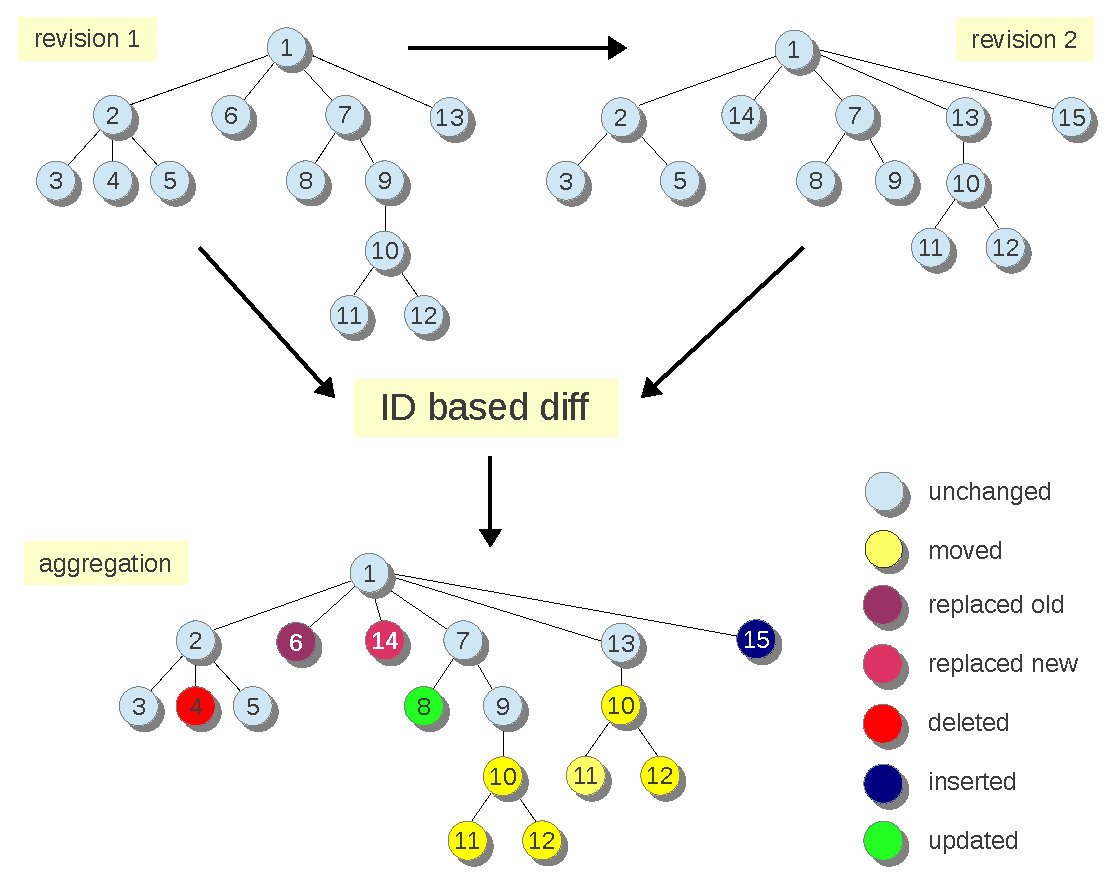
\includegraphics[width=\textwidth]
{figures/aggregation}}
\caption{\label{fig:aggregation} Two tree-structures aggregated. The numbers denote unique node-IDs and refer to Fig. \ref{fig:diff} in Chapter \ref{sec::differences} just like the changes from revision 1 to 2. Both revisions are input to the ID-based diff-algorithm. The output represents diff-tuples including the node-IDs from both nodes which are compared in each step, the type of diff and the depths of both nodes. Storing the observed diff-tuples in an ordered data-structure forms a tree-aggregation.}
\end{figure} 

\subsection{Visualizations}
Visualizations are a major contribution in this thesis. As described in the motivation humans are best in interpreting visual content. Therefore visualizations have been developed which facilitate humans in gaining new insights and quickly detecting differences in tree-structured data. Next, all available views are described in detail. %An XML based serializ   ation view of the tree-structure   %A few of them currently only support the visualization of one revision of the tree-structure. While not being of exceptional value for comparing trees besides viewing two instances of the GUI side by side they will most probably be extended to support

\begin{itemize}
\item
First, a \emph{TreeView} displays nodes in a tree structure just like visual frontends for filesystems as illustrated on the left side in Fig. \ref{fig:treetextview}. Nodes can be expanded to show all child nodes which are inside the current viewport or collapsed to hide children. Therefore a Java-Swing \texttt{JTree} is used which has been extended to mark the subtree of a selected node with a background color. The \texttt{TreeCellRenderer} renders nodes according to their node type and a \texttt{TreeModel} interacts with the storage. Currently the view is not able to incorporate the differences encountered via the diff-algorithm and therefore not further described.

\begin{figure}[tb]
\center{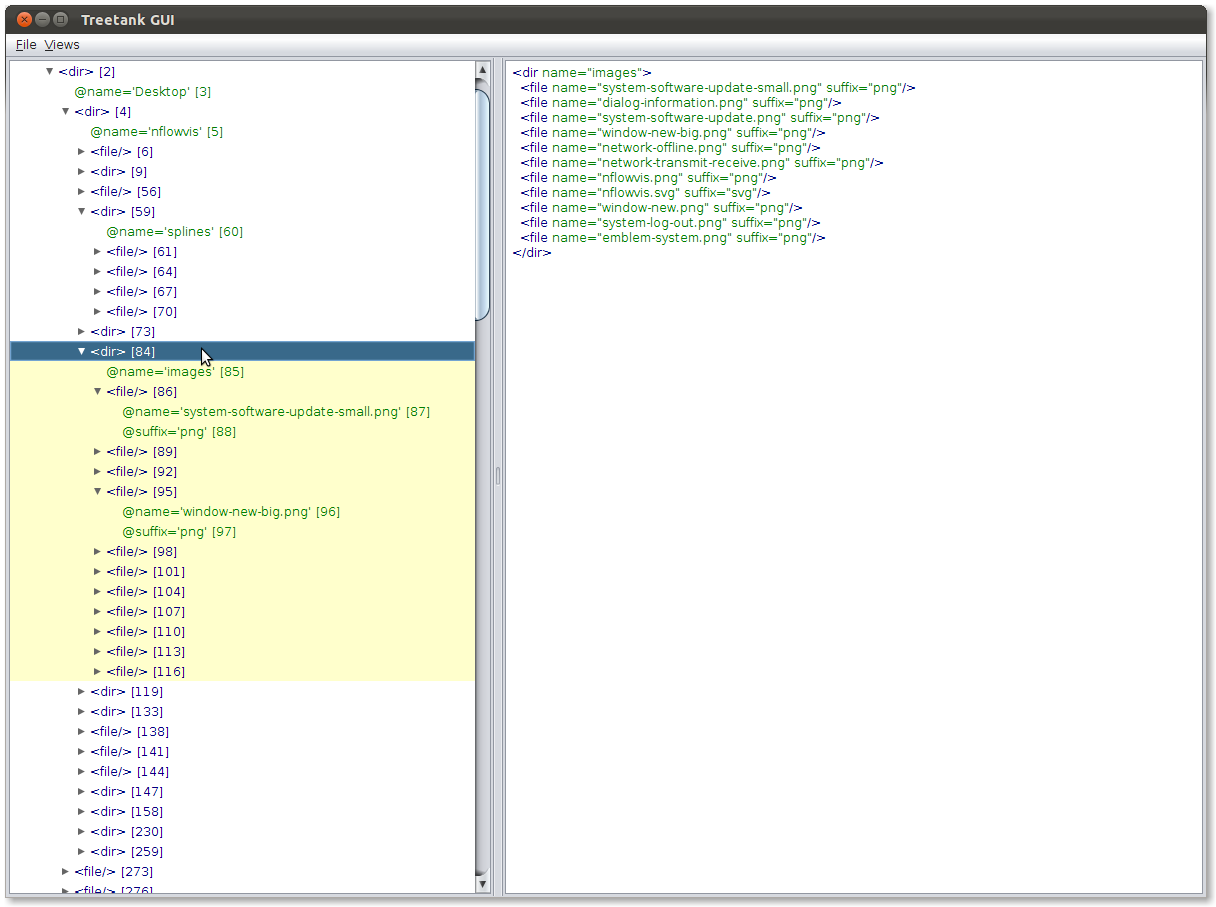
\includegraphics[width=\textwidth]
{figures/treetext}}
\caption{\label{fig:treetextview} TreeView and TextView side-by-side}
\end{figure}

\item
The \emph{TextView} displays serialized XML-documents or fragments and supports syntax highlighting. Moreover it just serializes the part of data which is currently viewable and an additional small overhead of pixels to enable scrolling. Other data is serialized and appended to the text pane once a user scrolls down. A new \emph{StAX}-parser implementation provides a pull-based API to support this "append-on-scroll" behaviour. It provides two features. Since it is pull based the application (the GUI) can determine when and how much data is parsed. Furthermore it provides the parsed node kinds which are used to support syntax highlighting. Simply using a \texttt{DescendantAxis} from Treetank which traverses the nodes in preorder would not be sufficient, end-tags have to be emitted as well. Therefore it is much easier to develop a reusable \texttt{StAX}-implementation. Nontheless the \texttt{DescendantAxis} is used internally as part of the implementation to traverse the tree in preorder. The algorithm which implements a StAX-Parser for Treetank is outlined in appendix \ref{Algorithm}. To adhere to the specifications of the methods which must be implemented and to keep the iterator-methods idempotent might have been the biggest challenge. In addition to generate events for end-tags the StAX-parser supports a \texttt{peek()}-method.

Figure \ref{fig:treetextview} displays the \emph{TreeView} and the \emph{TextView} side by side. Note that the two views are kept in synchronization.

In order to support an analyst with the task of analysing differences in tree-structured the view supports another mode which incorporates the aggregation of the two tree-structures to compare described in section \ref{subsec::aggregation}. Based on this aggregation another StAX-Parser called \emph{StAXDiffSerializer} has been developed which receives a \texttt{DiffAxis} to iterate over \texttt{SunburstItems} created for the \emph{SunburstView} which is described next. We support a preorder-traversal of the items to derive the stored diff-types as well as the depths in the items without the distortion of a semantic view for the \emph{SunburstView} described later on in this chapter. The depth of the current item and the depth of the next item using a \emph{peek()} method on the \texttt{DiffAxis} are used to determine if an end-tag must be emitted. Another check involves empty-Elements whereas an \texttt{EndElement} must be emitted immediately following the \texttt{StartElement} in the case of the next call to \texttt{nextEvent()}. In this case the parent node-IDs must match. Furthermore the depths are used in subsequent calls to \emph{nextEvent()} to determine how many closing tags must be emitted. In case of \texttt{ElementNode} updates we immediately emit the new updated element and push the old element on an end-tag stack. In a subsequent call to \texttt{nextEvent()} the old value in case of a \texttt{TextNode} or the old element in case of an \texttt{ElementNode} are emitted. Changed nodes are highlighted with a background color which denotes the kind of change. The \texttt{TextView} itself must not change the indentation for the old value/old element if an UPDATE has been detected. Only the first emitted value (the new value) must change the indentation. 

A legend which describes the color $\leftrightarrow$ change mapping is currently only available from within the \emph{SunburstView} which is described next. However this is only an implementation detail and a help-dialog can be added easily. Exemplary a side-by-side view with the \emph{SunburstView} is depicted in Fig. \ref{fig:sunbursttextview} whereas the first inserted subtree is also visible in the \emph{TextView} area. Note that while the SunburstView provides a great overview about the whole tree-structure and subtrees, the \emph{TextView} provides a better detailed view on selected parts of the whole tree-structure. Other deficiencies meantioned in the introduction regarding the boundary of nodes and XML-specific details do not apply as we compare the tree-structure, instead of a character based comparsion, with the ID-based diff-algorithm in the first place. Besides the lack of an appropriate overview, which is one of the advantages of the \emph{SunburstView}, the \emph{TextView} is an ideal partner to the \emph{SunburstView} as the XML text-serialization is better readable than radial Sunburst labels and readers might be more familiar with pure XML.

Note that the diff-algorithm is only ever called once for every visible view (besides a smallmultiple variant which represents changes among several tree-structures or revisions in Treetank), whereas a simple iterator on the created \emph{SunburstItem}s is broadcasted to all other views which are currently visible to support the iteration over the agglomerated tree-structure.

\begin{figure}[tb]
\center{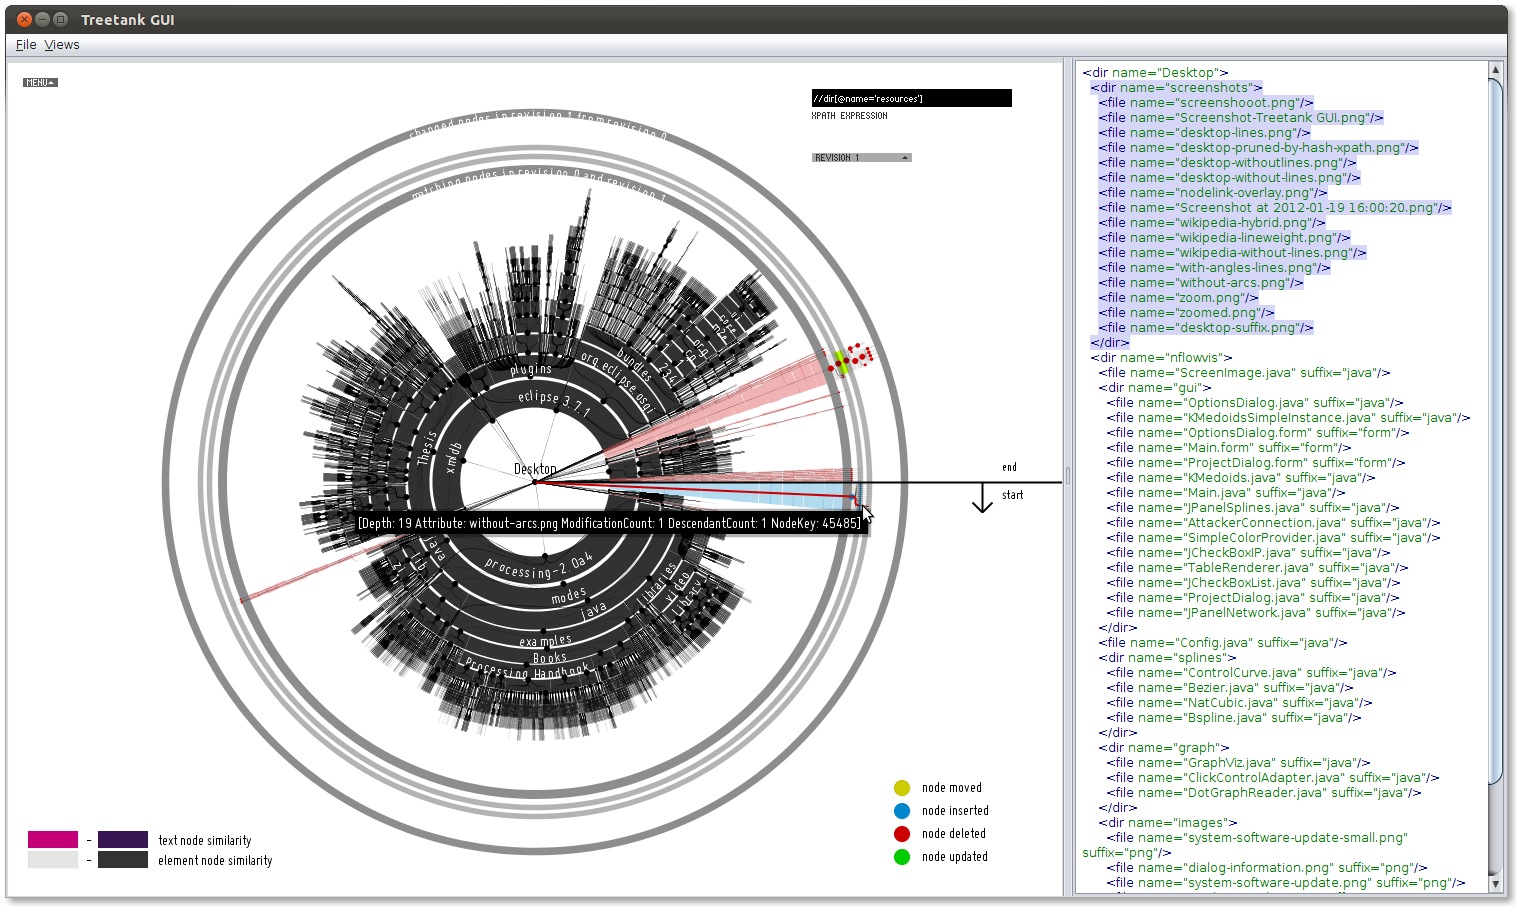
\includegraphics[width=\textwidth]
{figures/sunbursttextview-overview}}
\caption{\label{fig:sunbursttextview} SunburstView and TextView side-by-side}
\end{figure}

\item
The \emph{SunburstView} displays the tree structure in a radial arrangement. It is a space filling approach which tries to maximize available screen space for the hierarichical visualization. Furthermore it is adjacency based drawing child nodes next to their parent node. In contrast Treemaps enclose child-nodes within parent nodes. Thus a Treemap utilizes available screen space to the full extend as the root node uses all available space recursively embedding descendants as rectangles. In the Sunburst method unlike in Treemaps the corners are left empty due to the radial representation. While this alone on first glance might be a great drawback in addition to circular segments which are more difficult to read regarding size and the labels, the layout is stable even with a lot of changes and the hierarchical structure is much better readable. The Spiral Treemap layout which has been described in chapter \ref{sec::relwork} is relatively stable but it is still very difficult to track changes which might be scattered through a 45° degree change in direction as well as the complicacy to follow nested rectangles which are arranged in spirals compared to the simplicity of a Sunburst layout.

The root node of a tree-structure is plotted in the middle of the screen depicted as a circle. Child-nodes of the root node are plotted in circular segments next to their parent. In our case the radius depends on the depth and shrinks for an increasing depth such that the full circular area between two levels does not change. Otherwise items toward the edged will occupy more space. However this behaviour can be changed which is of importance to visualize changes which will be visualized along the edge (section \ref{subsec::comparison}). The extend of an item in the Sunburst layout which depicts one node depends on an attribute of the node whereas a relative measure in regard to the other children is used.  

The \texttt{SunburstView} is displayed in Fig. \ref{fig:sunburstview}.

\begin{figure}[tb]
\center{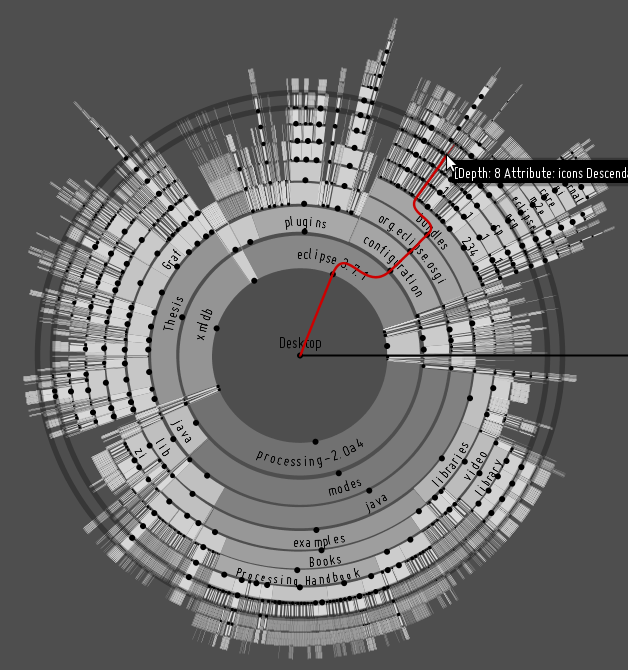
\includegraphics[width=\textwidth - 5em]
{figures/sunburstview-cut}}
\caption{\label{fig:sunburstview} SunburstView}
\end{figure}

The number of descendants of a node plus one is mapped onto the extend of each segment such that nodes having more descendants have a greater arc and therefore get more space. The formular is straight forward:

\begin{equation}
ext = \left\{ \begin{array}{cl}
2 \cdot \pi & \textrm{if }node\ is\ root\ node\\
parExt \cdot descs / (parDescs - 1) & \textrm{otherwise}\end{array}\right.
\end{equation}

Note that recently we have added the number of descendants of each structural node in Treetank itself to maximally speed up the creation of the visualization. Before, while creating the items we issued a preorder traversal on each node in parallel using the Java \texttt{ExecutorService} and a \texttt{BlockingQueue} which is also used in the comparsion view described later.

%\begin{equation}
%currExt = parExt * descCount / parDescCount
%\end{equation}

The color of each segment in case of internal nodes (element nodes) is mapped to the number of descendants of a node plus one as well. Having that said in future versions it will be possible to map another custom attribute available through a drop-down menu to the color. If such an attribute is not available for every node a default value can be assumed. Leaf nodes which are \texttt{text-nodes} are colored according to their text-length.

A node-link diagram is drawn on top of the \emph{SunburstView} to further emphasize the hierarchical structure. Dots representing the node in addition to the SunburstItem-segments are depicted in the middle of the segment whereas either bezier curves or straight lines denote a child/parent-relationship between the nodes.

In order to support large tree-structures the generated Sunburst-segments are drawn into an offscreen buffer, whereas the actual items are only used to implement a mouseover effect and to enable XPath-queries and highlighting of result-nodes.

\subsubsection{Interaction}
The view is highly customizable. Through checkboxes the dots/circles and/or the arcs can be hidden as well as the radius of the arcs can be adjusted through sliders. Moreover the size of the dots can be managed through a slider, whereas the connections between child/parent-nodes in the node-link overlay either can be disabled or a range denoting the line/curve thickness is adaptable. By default links at a higher level are drawn in thicker depending on the range. Furthermore color values for thecan be changed for the arcs , the background color, which also automatically adjusts legend text-colors to white if the background-color is very dark. On top of that it's possible to adjust the values such that either the whole node-link diagram or the \emph{SunburstView} disappears. Some adjustments are depicted in Fig. \ref{fig:sunburst-adjusted-scale}.

\begin{figure}[tb]
\center{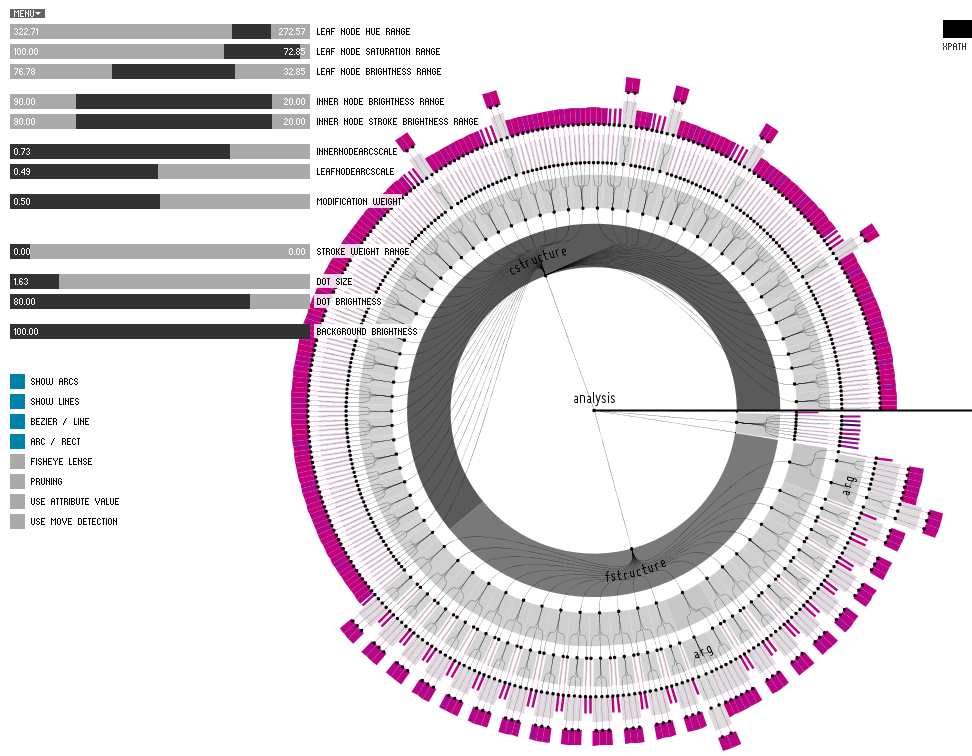
\includegraphics[width=\textwidth]
{figures/sunburst-adjusted-scale-cut}}
\caption{\label{fig:sunburst-adjusted-scale} SunburstView - adjusted arcs/dotsize parameters}
\end{figure}

Figure \ref{fig:nodelink} illustrates the node-link overlay without coloring the arcs. The red curve marks a path up to the root-node through all ancestor-nodes for the current node which is highlighted by moving the mouse over the item.

Besides, mapped values to the color of Sunburst-segments or items, a term which is used interchangeably in the following sections, can be normalized according to a linear, squareroot or logarithmic scale.

\begin{figure}[tb]
\center{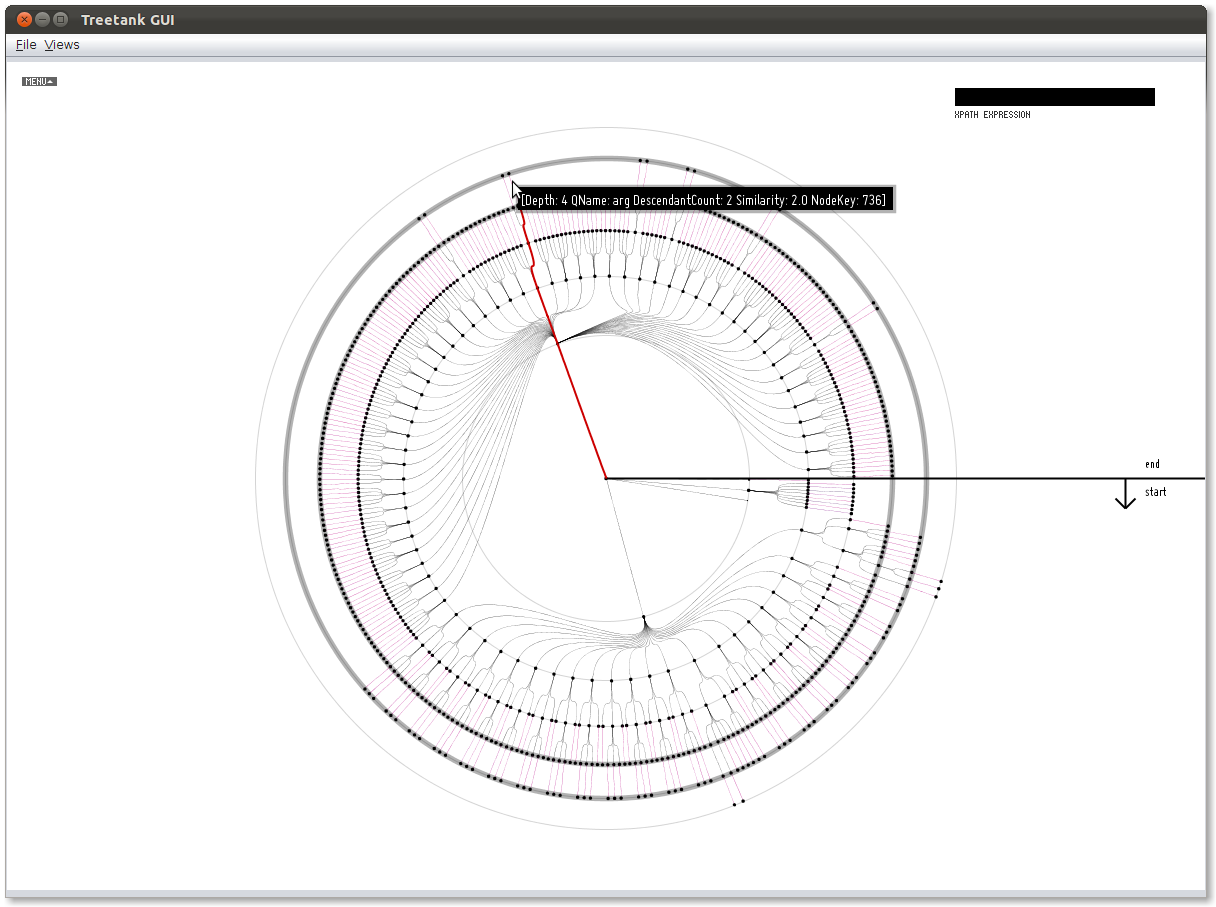
\includegraphics[width=\textwidth]
{figures/nodelink}}
\caption{\label{fig:nodelink} node-link diagram}
\end{figure}

Crucial to the interaction and the value of the visualization itself is the possibility to drill down into the tree. Clicking an item results in drawing the selected node with its subtree in a new Sunburst-diagram whereas the selected node is simply used as the new root-node. Stacks are used to implement a simple undo-operation which is very fast as we store the Sunburst-items as well as the background buffer-image. 

A well known technique to enlarge small regions is to use transformations of the screen-space, as for instance a fisheye lense. The enlargement of small items via a fisheye lense is depicted in Fig. \ref{fig:fisheye}. Zooming and panning is also incorporated allowing affine transformations of the screen (Fig. \ref{fig:zoom}) to analyse important regions. Note that the mouseover-effect displaying additional information about the node itself as well as the legends are not affected by the transformation. As the background-buffer cannot be used in this case zooming is restricted to smaller trees with an upper bound of about 10\_000 to 15\_000 nodes.

\begin{figure}[tb]
\center{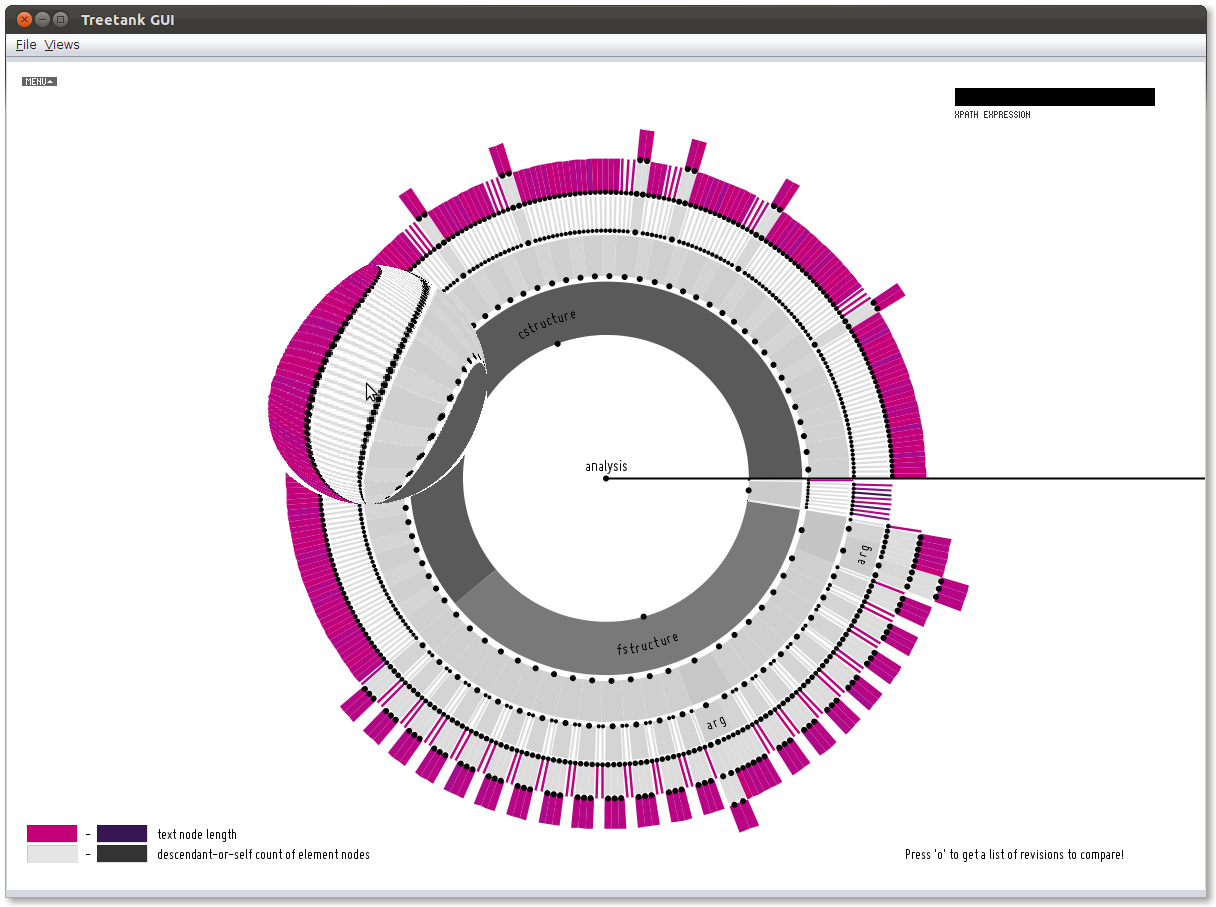
\includegraphics[width=\textwidth]
{figures/fisheye}}
\caption{\label{fig:fisheye} Fisheye transformation}
\end{figure}

\begin{figure}[tb]
\center{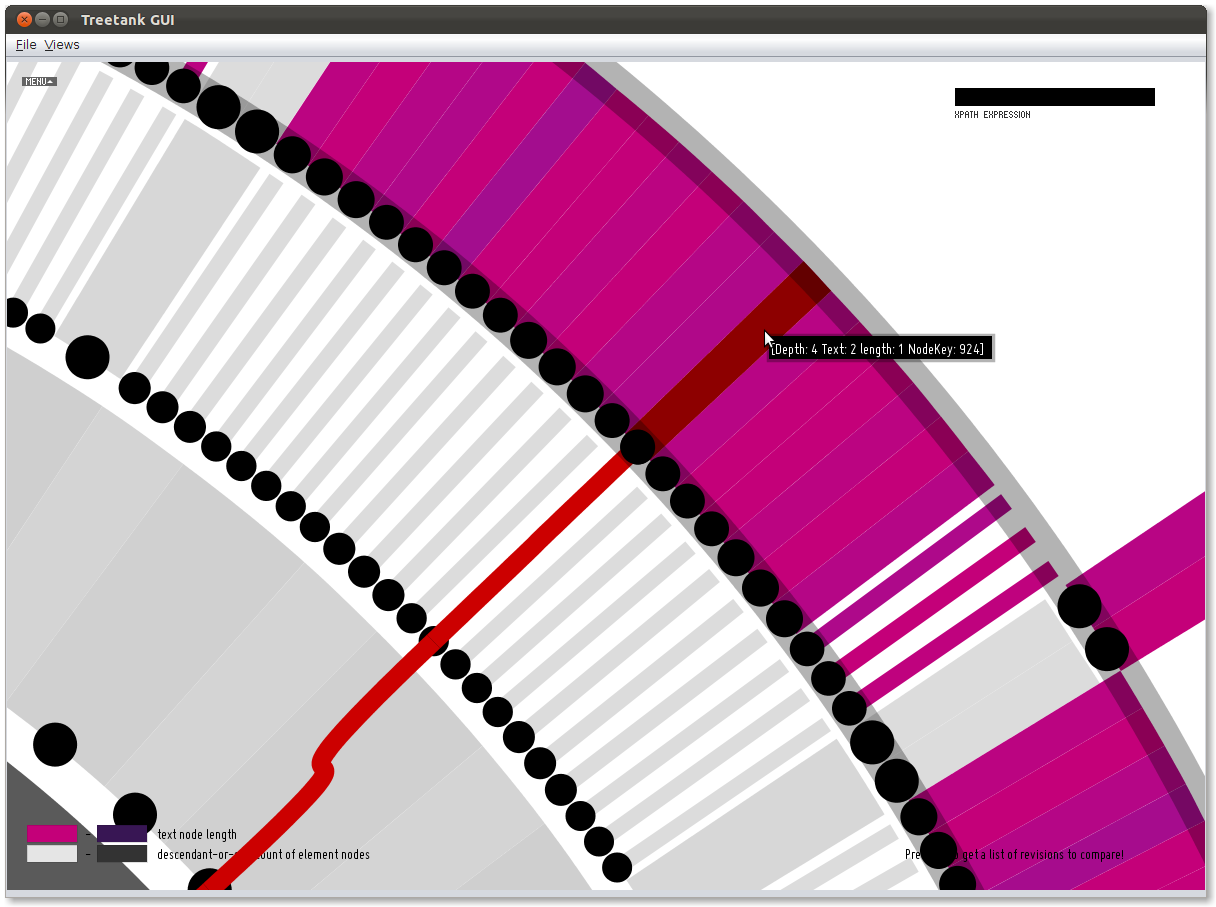
\includegraphics[width=\textwidth]
{figures/zooming}}
\caption{\label{fig:zoom} Zooming into the visualization}
\end{figure}

In order to manipulate Treetank resources it is even possible to insert XML fragments as right-siblings or first-childs as well as to delete nodes.

\subsubsection{Querying}
XPath can be used to query the tree-structure for specific nodes. Result sequences are highlighted in a light green. Figure \ref{fig:sunburstxpath} displays the result of a simple \texttt{//*[text()='var:0']} query to highlight all nodes which have a text-node child with the value "var:0".

\begin{figure}[tb]
\center{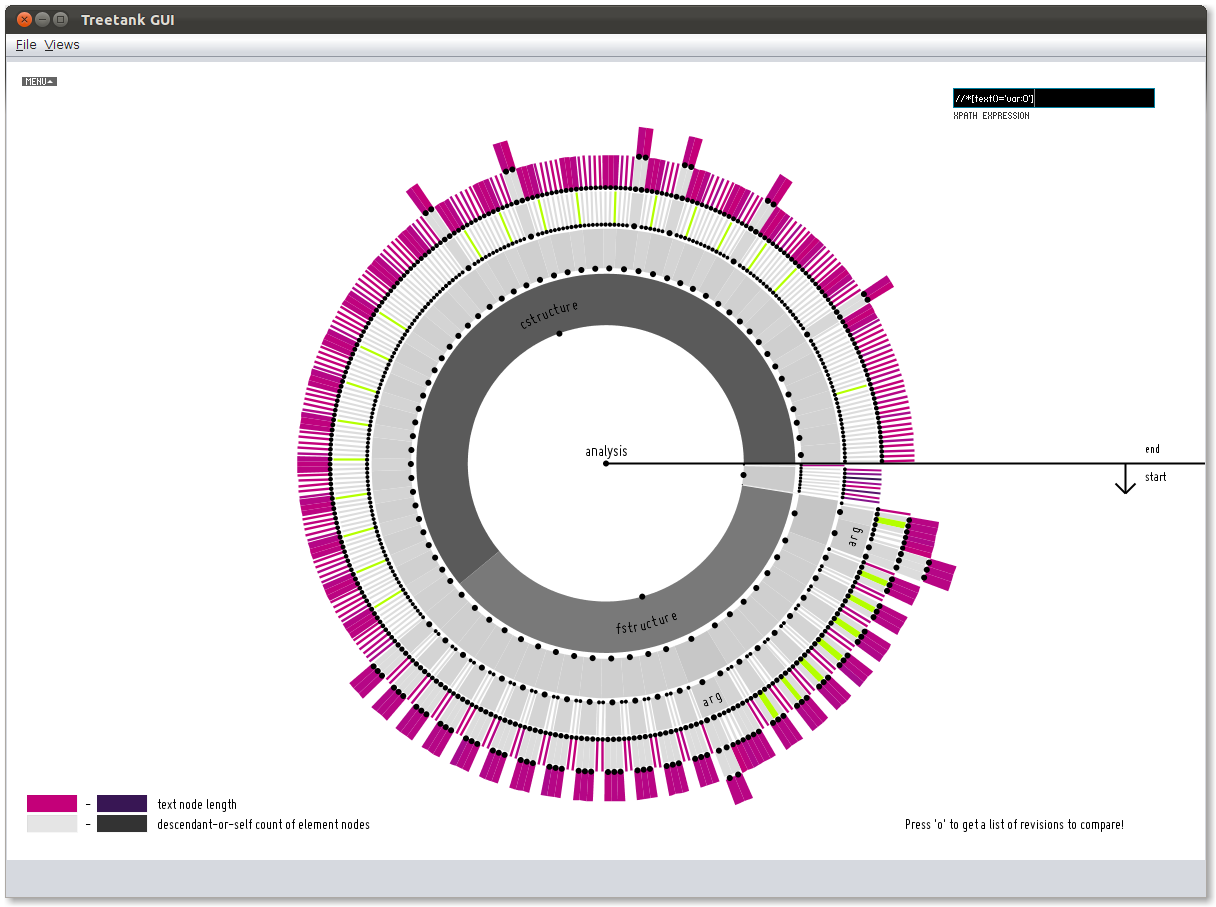
\includegraphics[width=\textwidth]
{figures/sunburstxpathquery}}
\caption{\label{fig:sunburstxpath} XPath query results displayed in light green}
\end{figure}

\subsubsection{Labels}
If the Sunburst items are huge enough and the scale to draw the arcs for each depth is greater than a predefined value (currently 0.7, whereas the scale ranges from 0 to 1) labels are drawn. Labels in the top half of the visualization, that is if the center of the item is greater than $\pi$, are drawn beginning at the startAngle in clockwise direction, otherwise they are drawn starting from the endAngle in counter clockwise direction. Furthermore the font-size ranges between two values, whereas the size is decreased with an increasing level. 

\subsubsection{Filtering/Pruning}
The standard \emph{SunburstView} incorporates a method to filter the tree by level. While this filtering is not perfect in circumstances where the fanout is very large, it turned out to work very well to keep the number of generated Sunburst items small. Furthermore the view currently is used as an entry point to the comparsion view which is also based on the Sunburst-layout whereas it is planned to backport the filtering by itemsize. In the following we use the terms \emph{filtering} and \emph{pruning} interchangeably.

Whereas it will be sufficient to use an XPath-query as for instance \\
\texttt{//*[count(ancestor::*)<3]} to get a sequence including all nodes between level 0 and 3 we opted for a tree-traversal implementation, as the XPath query has to touch all ancestor nodes in the current Treetank implementation which doesn't incorporate hierarchical node-IDs as for instance the ORDPATH/Dewey-IDs where it's usually trivial to compute such queries on the ID itself in an in-memory B*-tree or something alike. To support such queries efficiently it is scheduled to include the depth for each inserted node, which usually doesn't have to be adjusted in case of all operations but the movement of nodes/subtrees. In that case all moved nodes have to be adjusted instead of just the root node and it's former siblings/parent and the new siblings/parent. Furthermore the \texttt{DescendantAxis} and/or \texttt{VisitorDescendantAxis} can be adjusted to optionally use a maximum depth for the traversal.
\end{itemize}

\subsection{Comparsion using a new Sunburst-layout algorithm}\label{subsec::comparison}
The standard \emph{SunburstView} includes a comparison-mode. Once a base revision is opened and the \emph{SunburtView} is enabled an analyst is able to choose another revision from a dropdown menu for comparison. Note that all interaction capabilities described earlier are also available in the comparison mode. Differences and additional capabilities are described in the following sections. In order to compare tree-structures in a radial arrangement similar to the described "usual" SunburstView to explore a single revision a new layout-algorithm has been developed. Next, we first describe the new layout.

\subsubsection{Sunburst Comparsion-Layout}
The Sunburst comparison layout is illustrated in Fig. \ref{fig:sunburst}. Nodes are colored as depicted in the color legend in the bottom right corner. All nodes which have not changed as part of comparing the base revision to another revision\footnote{in this case revision 1} are plotted inside the inner circle which is labeled "matching nodes in revision 0 and revision 1". The circle itself is drawn between the maximum level of the unchanged nodes plus one and maxLevel plus two. Changed nodes are zoomed out from their original place and drawn between the two dark circles labeled "changed nodes in revision 0 and revision 1" and "matching nodes between revision 0 and 1". To demonstrate the area denoting the changes it is hatched in Fig. \ref{fig:sunburst}. Similarly the arrows emphasize the direction in which changed subtrees are zoomed/dislocated. This semantic zoom serves a double purpose. First, the visualization adheres to a Tree-Ring metapher depicting the evolution of a tree. Like the age of a tree in the nature is deducable by analysing rings in a cross-cut of the stem whereas the rings denote the age and each ring represents one year starting from the very middle to the outside, our representation aims at representing the changes between two rings. In our representation the unchanged nodes form the middle of the \emph{SunburstView} whereby changed nodes are zoomed to the border between the outer and inner ring which is representing the growth of a tree in case of analysing temporal tree-structures. Additionally this transformation of changed subtrees displaces these subtrees to a prominent place. Small changed subtrees are thus much better noticeable as they are not surrounded by unchanged subtrees which might even be deeper. To depict changes between multiple trees first considerations involved the addition of changes from a sequence of sorted revisions in further circles around the one denoting the changed nodes. That is, the inner circle represents unchanged nodes between \emph{all} compared revisions whereas changes between selected or consecutive revisions are drawn between new outer rings which are appended. According to the Tree-Ring metapher each comparison between a pair of trees would append a new rings for their changes. However this would affect the whole layout each time. The idea proved to be not viable because of the complexity this involves. To name a few

\begin{itemize}
\item The inner ring must keep space between unchanged nodes/subtrees for all changed subtrees in the outer rings.
\item Consecutive calling the diff-algorithm and merging diffs into a diff-list with diff-tuples which has already been created.
\item Keeping track of all opened transactions and resetting the transaction appropriately depending on the revision in which a change has occured.
\item Similarly the depth for items in the tree will change very often which involves further state and it is almost not possible to denote the current depth.
\item The \texttt{descendant-or-self}- and \texttt{modification}-count of each nodes' subtree will be cumbersome to calculate.
\end{itemize}

\begin{figure}[tb]
\center{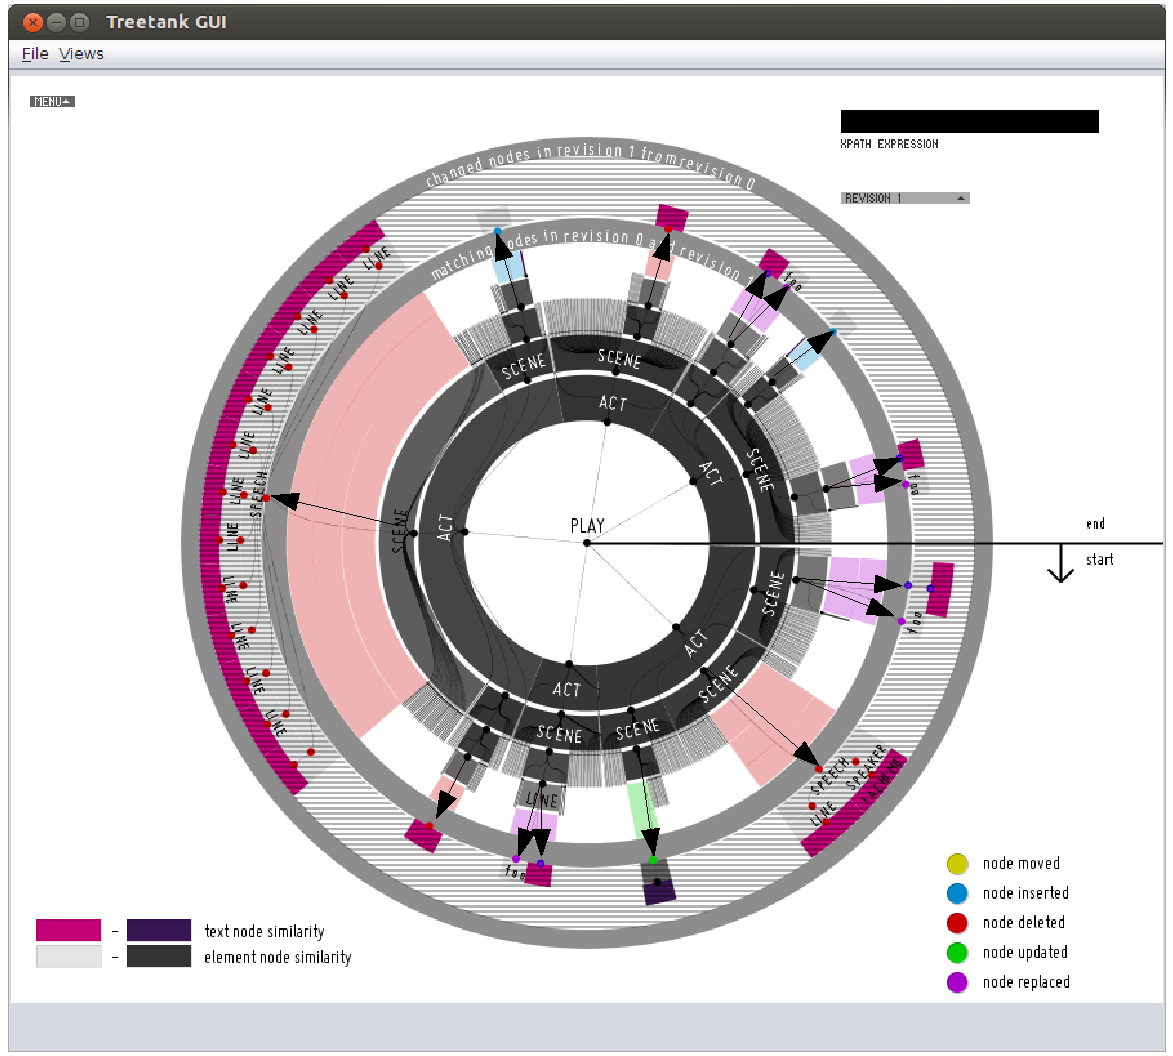
\includegraphics[width=\textwidth]
{figures/sunburst.pdf}}
\caption{\label{fig:sunburst} SunburstView - comparison mode.}
\end{figure}

These and similar complexity considerations formed the idea of introducing Small multiple visualizations of the current view which are described in section \ref{subsec::smallmultiple}.
Adhering to the Tree-Ring metapher, the semantic zoom surves the purpose that all changed nodes are visible on first glance. Otherwise it would be hard to track small changes. 

\subsubsection{Short animation}
In order to clearly demonstrate the semantic zoom a short animation has been implemented as test persons usually did not grasp the meaning without further explanation. Thus the transformation of changed subtrees is shown which dislocates the items to their dedicated positions along the arrows in Fig. \ref{fig:sunburst} \footnote{remember, the arrows are not drawn in the visualization, they have been added to the screenshot to emphasize the transformation}. However the animation is only drawn if the framerate will not drop due to too many items. Thus when a certain amount of items has been created the animation will be skipped.

\subsubsection{Layout algorithm}
After invoking the ID-based diff-algorithm depending on the chosen filtering-method (described in the next section) the new Sunburst-layout has to be drawn. First of all, based on the generated aggregation of the trees, Sunburst items which denote the nodes in the aggregated tree have to be computed. The diff-tuple encountered through observing changes computed by the ID-based diff-algorithm is of the following form: key in first revision / key in second revision / depth in first revision / depth in second revision / kind of diff. The Sunburst items are created based on a special axis which implements the Iterator/Iterable interfaces from Java to traverse the diff-tuples. That is the following two methods are available: \texttt{hasNext()} and \texttt{next()}. Initially we developed an axis based on the idea of traversing the tree-structure just like in the \texttt{SunburstDescendantAxis} and to adjust a simple index-variable pointing to the next diff-tuple. The key idea is to traverse the tree-structure based on the transaction opened on the newer revision whereas usually the pointers of the nodes are used as a guidance to traverse the aggregated tree-structure in document-order. The transaction will be changed to the old revision whenever a diff of type \texttt{DiffType.MOVEDFROM}, \texttt{DiffType.DELETED} or \texttt{DiffType.REPLACEDOLD} is encountered. However the preorder-traversal using a pointer-based approach similar to the algorithms in the \texttt{SunburstDescendantAxis} or the \texttt{DescendantAxis} itself bares a lot of complexity as the node key of the next node to traverse has to be set in advance and the movement of the transaction in a lot of cases cannot be immediately reflected by adjusting certain stacks which are required to determine the start-Angle, extend, descendantCount, modificationCount and the parent index. In fact in some cases the adjustments can not be done until the next call to \texttt{hasNext()}. Figure \ref{fig:tree-axis} demonstrates a lot of this complexity on a simple tree-aggregation. Note that the terms "aggregation" and "agglomeration" are used exchangeable in this thesis. 

\begin{figure}[tb]
\center{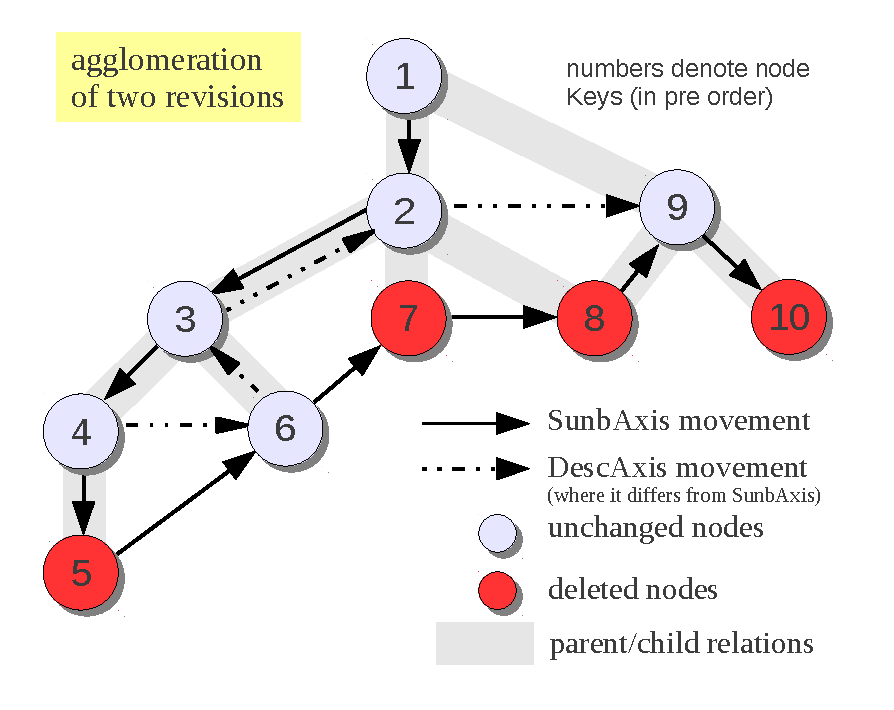
\includegraphics[width=\textwidth - 12.5em]
{figures/tree-axis}}
\caption{\label{fig:tree-axis} SunburstCompare-Axis based on the Sunburst-Axis}
\end{figure}

If the transaction-cursor is located at the node with the nodeKey 4 in the new revision the next nodeKey will be the node denoted by nodeKey 6 in the \texttt{Descendant}- and the \texttt{Sunburst}-axis as node 5 is deleted. As such the simple expression $rtx.getStructuralNode().hasFirstChild()$ to test for a child node must be extended to keep track of these issues, for instance by receiving the next element in the diff-list and compare the diff to the type \texttt{DELETED} and \texttt{MOVEDFROM} whereby the depth must be greater than the current depth. Furthermore the kind of movement must be tracked just like in the \texttt{SunburstDescendantAxis} to adjust the stacks with the start-angle, extension, depths and descendant- as well as modification-number accordingly. Everytime before a new SunburstItem is added to a list which contains all resulting items in the end, the values as for instance the descendant-or-self number and the modification-number as well as the startAngle/extension must adapted based on the stacks which have to be adjusted themselfes depending on the transaction movement. 

Another example of the complexity is the movement from node 6 to node 9 in the normal \texttt{DescendantAxis} whereas in our case the next node is the deleted node 7. Thus the \texttt{pop()}-method on the stacks must be called once instead of two times. Each time a \texttt{DELETED} or \texttt{MOVEDFROM} diff kind is encountered the transaction is temporarily changed along with the nextNodeKey which denotes the key the $hasNext()$-method must move to the next time called and a right-sibling node stack which is used in cases where the node has no first child and no right sibling. In this case the next nodeKey is popped from the right-sibling stack (a nodeKey is pushed on the stack for each child-movement whenever the node before the move to the first child has a right sibling) and as in the algorithm \ref{algo:popStacks} the depth must be considered too, that is like in the example scenario described before such that the pop()-method is called the right number of times. This method is invoked for the first \texttt{DELETED} or \texttt{MOVEDFROM} after another diff-kind has been encountered. If the movement of the transaction before calling this method was of kind \texttt{EMoved.ANCHESTSIBL}, that is the transaction will be moved to the right sibling of the first ancestor which has one. This cannot be done until the next call to $hasNext()$ as otherwise the stacks will not be adapted appropriately. Note that the first while-iteration doesn't call pop() as no values have been pushed on the stacks for leaf-nodes. Another remark concerns the else-branch which is executed if the depth of the current node in the list is equal or even greater than the last depth.

Similarly if the movement-type was to a right sibling of the first anchestor-node which has one and the next node will not be of the kind \texttt{DELETED} and \texttt{MOVEDFROM}, the actual movement cannot be done before the next call to $hasNext()$ and the method is very similar to algorithm \ref{algo:popStacks}.

\begin{algorithm}[Hhtbp]
%\SetAlgoLined
\SetKwInOut{Input}{input}\SetKwInOut{Output}{output}
\Input{instance variabled denoted by a trailing m, int initDepth, Diff lastDiffCont, EMoved moved}
\Output{nothing, the instance variables are directly modified (method/algorithm has side effects)}
\BlankLine
int tmpDepth = 0\;
\If{mDepth == 0}{
  tmpDepth $\leftarrow$ initDepth\;
}\Else{
  tmpDepth $\leftarrow$ lastDiffCont.getDepth().getNewDepth()\;
}
\If{mMoved == EMoved.ANCHESTSIBL}{
  \If{tmpDepth - mInitDepth $>$ diffCont.getDepth().getOldDepth() - initDepth} {
    \tcp{Must be done on the transaction which is bound to the new revision.}
    boolean first $\leftarrow$ true\;
    \While{tmpDepth - initDepth $>$ diffCont.getDepth().getOldDepth() - initDepth} {
      \If{first == true}{
        \tcp{Do not pop from stack if it's a leaf node.}
        first $\leftarrow$ false\;
      }\Else{
        mDiffStack.pop()\;
        mAngleStack.pop()\;
        mExtensionStack.pop()\;
        mParentStack.pop()\;
        mDescendantsStack.pop()\;
      }

      tmpDepth--\;
      mDepth--\;
    }
  }\Else{
    moved $\leftarrow$ EMoved.STARTRIGHTSIBL\;
    mAngle += mExtension;
  }
}
\caption{adjusting stacks and depths for movement to next following node for the first DELETED or MOVEDFROM node after another type has been encountered}\label{algo:popStacks}
\end{algorithm}

The last pitfall in Fig. \ref{fig:tree-axis} is after traversing the node denoted by nodeKey 9. Usually $hasNext()$ will return false but in this case it must return true, as the deleted node "10" follows.

We observed that the overall algorithm is very complex in terms of a lot of special cases as described in the last paragraphs have to be considered which directly results in many comparsions and instructions and therefore might be a performance issue as well.

The complete algorithm therefore is not described as recently a new, in comparsion, lightweight algorithm has been developed. Instead of using a pointer based traversal it became apparent that it is easier to directly use the diff-tuple and move either the transaction on the old revision or the transaction on the new revision depending on the diff-kind. In case of a \texttt{DELETED} or \texttt{MOVEDFROM} the working transaction is based on the transaction opened on the old revision, otherwise the transaction opened on the new revision is used.

The algorithm skeleton for $hasNext()$ is described in \ref{algo:skeleton}.
\begin{algorithm}[Hhtbp]
%\SetAlgoLined
\SetKwInOut{Input}{input}\SetKwInOut{Output}{output}
\Input{instance variabled (denoted by a trailing m)}
\Output{true, if more diffs are in the diff list, false if index == size}
\BlankLine
\tcp{Fail if there is no node anymore.}
\If{!mHasNext}{
  return false\;
}

\tcp{Setup everything.}
setupDiffs()\;

\If{mIsOldTransaction == true}{
  setTransaction(mOldRtx)\;
}\Else{
  setTransaction(mNewRtx)\;
}

\tcp{Move to next key.}
getTransaction().moveTo(mNodeKey)\;

\If{mHasMorDiffKinds == true}{
  \If{mDiff == DiffKind.UPDATED OR mDiff == DiffKind.REPLACEDOLD}{
    \tcp{For DiffKind.UPDATE or DiffKind.REPLACED the transaction needs to be on the right node.}
    mOldRtx.moveTo(mDiffCont.getOldNodeKey())\;
  }

  \tcp{Always follow first child if there is one.}
  \If{mNextDepth $>$ mDepth}{
    return processFirstChild()\;
  }

  \tcp{Then follow right sibling if there is one.}
  \If{mDepth == mNextDepth}{
    return processRightSibling()\;
  }

  \tcp{Then follow next following node.}
  \If{mNextDepth $<$ mDepth}{
    return processNextFollowing()\;
  }
}
\tcp{Then end.}
processLastItem()\;
mHasNext $\leftarrow$ false\;
return true\;
\caption{Diff-Axis hasNext()-skeleton}\label{algo:skeleton}
\end{algorithm}

The method \texttt{setupDiffs} takes care of setting the current depth which depends on the diff-kind/type, the upcoming next depth, if the list has more diff-elements as well as setting the boolean instance variable \texttt{mIsOldTransaction} which is \texttt{true} if the diff-kind is of type \texttt{DELETED}, \texttt{MOVEDFROM} or \texttt{REPLACEDOLD} and \texttt{false} otherwise. After determining which transaction must be used based on \texttt{mIsOldTransaction} if more elements are in the diff-list the transaction is moved to the next key determined by the diff-kind and obtained from the diff-element, the tuple described earlier which incorporates the nodeKey of both nodes which have been compared in the diff-algorithm as well as the depths of both nodes. In order to provide both the old value and new value\footnote{in case of a \texttt{TextNode}} or QName\footnote{in case of an \texttt{ElementNode}} in the case of updates and similarly in case of replaces for the next SunburstItem, the transaction opened on the base revision which is always the older revision is moved to the node key of the node in the old revision. Note that this information is available from the diff-tuple. Thus both transactions are located at the right nodes. The following three \texttt{if}-clauses ensure the preorder traversal of the axis. If the next depth is greater than the current depth the next node is a child node in the agglomerated tree, thus the variables of the last created Sunburst item which depend on the stacks must be pushed on top of these. As in all cases the variable which denotes the movement must be adapted. Otherwise if the next depth is equal to the current depth the next node is a right sibling. In this case the extension of the last emitted Sunburst item has to be added to the startAngle and the movement variable must be adjusted accordingly. Likewise if the next depth is lower than the current depth the next node is a right sibling of the first ancestor which has an appropriate pointer (!= $NULL\_NODE\_KEY$ which denotes that no right sibling is available). Thus the stacks must be adapted similar to algorithm \ref{algo:popStacks}. Algorithm \ref{algo:nextitem} describes how the stacks, depending on the last movement, are used to adapt dependent variables for the next Sunburst item.

\begin{algorithm}[Hhtbp]
%\SetAlgoLined
\SetKwInOut{Input}{input}\SetKwInOut{Output}{output}
\Input{IReadTransaction pRtx, Item pItem, Stack pAngleStack, Stack pExtensionStack, Stack pParentStack, Stack pDescendantStack}
\Output{nothing, executed for it's side effects, that is adapting stacks and an item to create a Sunburst Item afterwards}
\BlankLine
\If{lastMovement == START\_OR\_RIGHTSIBL}{
  \tcp{Do nothing.}
}\ElseIf{lastMovement == CHILD}{
  pItem.mAngle $\leftarrow$ pAngleStack.peek()\;
  pItem.mExtension $\leftarrow$ pExtensionStack.peek()\;
  pItem.mIndexToParent $\leftarrow$ pParentStack.peek()\;
  pItem.mParentDescendantCount $\leftarrow$ pDescendantsStack.peek()\;
}\ElseIf{lastMovement == ANCHEST\_RIGHT\_SIBL}{
  pItem.mAngle $\leftarrow$ pAngleStack.pop()\;
  pItem.mAngle $+=$ pExtensionStack.pop()\;
  pItem.mExtension $\leftarrow$ pExtensionStack.peek()\;
  pParentStack.pop()\;
  pItem.mIndexToParent $\leftarrow$ pParentStack.peek()\;
  pDescendantsStack.pop()\;
  pItem.mParentDescendantCount $\leftarrow$ pDescendantsStack.peek()\;
}
\caption{Stack adaptions for next Sunburst item depending on transaction movement in last call of \texttt{hasNext()}}\label{algo:nextitem}
\end{algorithm}

\subsubsection{Semantic zoom implementation}
The implementation of the \emph{semantic zoom} with changes highlighted in a dedicated place requires an adaption of the depth of the first changed node in every subtree in a preorder-traversal of the agglomerated tree to reflect the changes in its dedicated position between the two rings. Three cases have to be distinguished in which the depth must be adapted (Fig \ref{fig:sunburst-layout}).

\begin{enumerate}
\item Transition from an unchanged node to the first changed node in a subtree (1) in Fig. \ref{fig:sunburst-layout}). 
\item Transition to another changed node once a (changed) subtree has been traversed and a node on the XPath \texttt{following::}-axis follows whereas its original depth would be less than the depth of the inner ring ($pMaxDepth + 2$) which only ever includes unchanged nodes (3) in Fig. \ref{fig:sunburst-layout}).
\item Transition from a changed node back to an unchanged node in case the unchanged node is not in the changed nodes' subtree. An unchanged node might only be in a changed nodes' subtree if the changed node has been updated (2) in Fig. \ref{fig:sunburst-layout}).
\end{enumerate}

\begin{figure}[tb]
\center{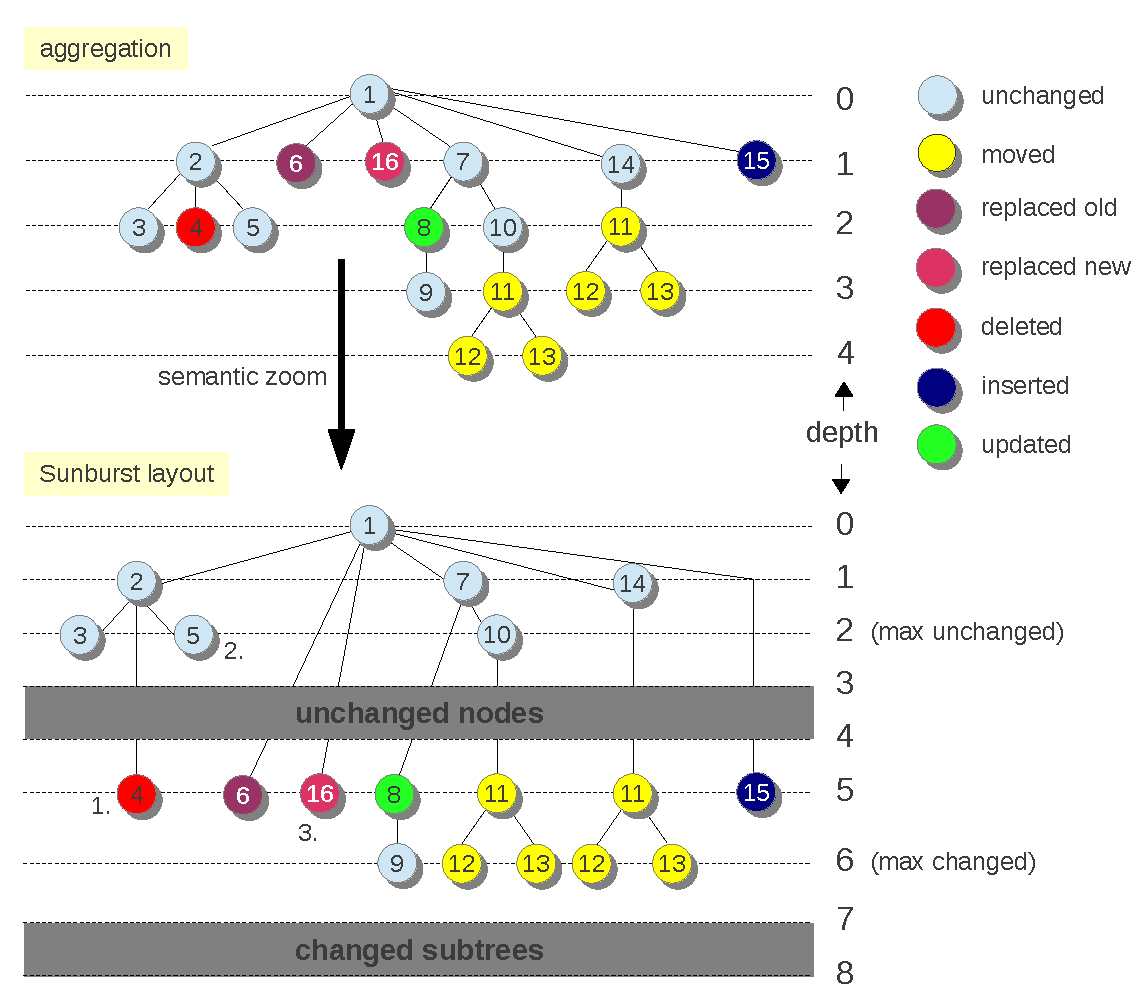
\includegraphics[width=\textwidth]
{figures/sunburst-layout}}
\caption{\label{fig:sunburst-layout} Sunburst-layout depicting changes in the depth. All nodes above the grey rectangle labeled "unchanged nodes" are unchanged whereas the area between the rectangle named "changed subtrees" includes all changed subtrees. However it also includes changed nodes below an updated node as for instance node 9.}
\end{figure}

Algorithm \ref{algo:calcDepth} determines if and how the depth must be adjusted. The first and second case is handled by the first \texttt{if}-clause, whereas the transition back to the original depth is handled by the \texttt{elseif}-clause. An instance variable \emph{mTempKey} is used to determine when to switch back. It is the node-ID of the first node in the XPath \texttt{following::}-axis which is not changed. However the variable always refers to the first node in the \texttt{following::}-axis which is changed in the second case. An \texttt{UPDATED} node most probably incorporates unchanged nodes if it is an internal \texttt{ElementNode}. In these cases we do not use the original depth of the node, but the current depth based on the tree traversal in the \texttt{Diff}-Axis which reflects the original depth plus the additional depth-difference to transform the depth of the first updated node.

\begin{algorithm}[Hhtbp]
%\SetAlgoLined
\SetKwInOut{Input}{input}\SetKwInOut{Output}{output}
\Input{int pDepth, DiffType pDiff, DiffTuple pDiffCont, int pMaxDepth, PruningType pPrune, instance variables denoted by a trailing "m" (long mTempKey, long mInitDepth)}
\Output{new depth}
\BlankLine
int depth $\leftarrow$ pDepth\;
\If{pDiff != DiffType.SAME AND pDiff != DiffType.SAMEHASH AND pDepth $\leq$ pMaxDepth + 2}{
  depth $\leftarrow$ pMaxDepth + 2\;

  int index $\leftarrow$ mIndex + mPrunedNodes + mDescendantCount\;
  boolean isOldTransaction $\leftarrow$ (pDiff == DiffType.DELETED OR pDiff == DiffType.MOVEDFROM OR pDiff == DiffType.REPLACEDOLD)\;
  DiffDepth depthCont $\leftarrow$ mDiffCont.getDepth()\;
  int depth $\leftarrow$ 0\; 
  \If{isOldTransaction == true}{
    depth $\leftarrow$ depthCont.getOldDepth()\;
  }\Else{
    depth $\leftarrow$ depthCont.getNewDepth()\;
  }

  \If{index $<$ mDiffs.size()}{
    Diff nextDiffCont $\leftarrow$ mDiffs.get(index)\;
    DiffType nextDiff $\leftarrow$ nextDiffCont.getDiff()\;
    boolean nextIsOldTransaction $\leftarrow$ (nextDiff == DiffType.DELETED OR nextDiff == DiffType.MOVEDFROM OR nextDiff == DiffType.REPLACEDOLD)\;
    DiffDepth nextDepthCont $\leftarrow$ nextDiffCont.getDepth()\;
    int nextDepth $\leftarrow$ 0\;
    \If{nextIsOldTransaction == true}{
      nextDepth $\leftarrow$ nextDepthCont.getOldDepth()\;
    }\Else{
      nextDepth $\leftarrow$ nextDepthCont.getNewDepth()\;
    }

    mTempKey $\leftarrow$ 0\;
    \If{nextIsOldTransaction == true}{
      mTempKey $\leftarrow$ nextDiffCont.getOldNodeKey()\;
    }\Else{
      mTempKey $\leftarrow$ nextDiffCont.getNewNodeKey()\;
    }
  }
}\ElseIf{(pDiff == DiffType.SAME OR pDiff == DiffType.SAMEHASH) AND pDiffCont.getNewNodeKey() == mTempKey}{
  depth $\leftarrow$ pDiffCont.getDepth().getNewDepth() - mInitDepth\;
}
return depth\;
\caption{Calculate depth}\label{algo:calcDepth}
\end{algorithm}

Besides adjusting the depth the semantic zoom requires some form of highlighting. In our case we opted for a global "distortion" which enlarges modified subtrees and shrinks subtrees of unchanged nodes. Thus, the extend of a Sunburst item depends on two variables, the \texttt{descendant-or-self}-count and the number of \texttt{modification}s in a nodes' subtree.

\begin{equation}
ext = \left\{ \begin{array}{cl}
2 \cdot \pi & \textrm{if }node\ is\ root\ node\\
parExt \cdot ((1-\alpha) \cdot descs / (parDescs - 1) \\+ \alpha \cdot mods / (parMods - 1)) & \textrm{otherwise}\end{array}\right.
\end{equation}

The modification-count in the forumla is derived from the \\ \texttt{descendant-or-self}-count added to the \texttt{modification}-count of the current node plus a constant. The addition of the \texttt{descendant-or-self}-count is needed to handle nodes, which do not contain any modifications in its subtree and the node itself is not changed, too. In order to further emphasize and enlarge subtrees with a small number of modifications a constant is added which has proven useful in empirical studies (Chapter \ref{sec::applications}). Futhermore note that if the parent node has been modified the constant must be subtracted from the parent \texttt{modification}-count in advance. Otherwise the equation will not work.

The two variables are computed in parallel to the \texttt{Diff-Axis}-traversal \\whereas the results are appended to a \texttt{BlockingQueue}, which is a thread safe queue designed for producer/consumer relationships. Modifications for the root node are gathered while observing diff-tuples, thus the modifcation-count does not need to be computed afterwards as for the other nodes in the agglomerated tree-structure. A simple heuristic determines depending on a depth-threshold if tasks are executed in the calling thread instead of another thread, as context switches for very small subtrees are too costly. Observe that the added descendant-count for each node can not be used, because the aggregated tree-structure is traversed which incorporates deleted and moved nodes. Algorithm \ref{algo:descModCount} depicts how the two variables are derived from traversing the diff-datastructure at a specified index until the depth of a diff in the agglomerated tree-structure either is less than or equal to the start depth or no more diff-tuples are following. Note that the depth depends on the diff-type. In case of a \texttt{DELETED}, \texttt{MOVEDFROM} or \texttt{REPLACEDOLD} diff-type the depth of the node in the older revision is used, otherwise the depth of the node in the new revision. Furthermore recapitulate that the depths are computed by the ID-based diff-algorithm instead of stored directly in the node by Treetank.

\begin{algorithm}[Hhtbp]
%\SetAlgoLined
\SetKwInOut{Input}{input}\SetKwInOut{Output}{output}
\Input{int pIndex, List pDiffs}
\Output{CONSTANT\_FACTOR * diffCounts, descendantCounts, subtract}
\BlankLine
int index $\leftarrow$ pIndex\;
DiffTuple diffCont $\leftarrow$ pDiffs.get(index)\;
DiffType diff $\leftarrow$ diffCont.getDiff()\;
int rootDepth $\leftarrow$ diffCont.getDepth().getNewDepth()\;
\If{diff == DiffKind.DELETED OR diff == DiffKind.MOVEDFROM OR currDiff == DiffType.REPLACEDOLD}{
  rootDepth $\leftarrow$ diffCont.getDepth().getOldDepth()\;
}

int diffCounts $\leftarrow$ incrDiffCounter(index)\;
int descendantCounts $\leftarrow$ 1\;
boolean subtract $\leftarrow$ false\;
diffCounts = incrDiffCounter(index)\;
index $\leftarrow$ index + 1\;

\If{diffCounts == 1 AND index $<$ mDiffs.size()}{
  DiffTuple cont $\leftarrow$ mDiffs.get(index)\;
  int depth $\leftarrow$ cont.getDepth().getNewDepth()\;
  \If{cont.getDiff() == DiffType.DELETED OR cont.getDiff() == DiffType.MOVEDFROM OR currDiff == DiffType.REPLACEDOLD}{
    depth $\leftarrow$ cont.getDepth().getOldDepth()\;
  }
  \If{depth == rootDepth + 1}{
    \tcp{Current node is modified and has at least one child.}
    subtract $\leftarrow$ true\;
  }
}

boolean done $\leftarrow$ false\;
\While{!done AND index $<$ mDiffs.size()}{
  DiffTuple currDiffCont $\leftarrow$ mDiffs.get(index)\;
  DiffType currDiff $\leftarrow$ currDiffCont.getDiff()\;
  DiffDepth currDepth $\leftarrow$ currDiffCont.getDepth()\;
  int depth $\leftarrow$ currDepth.getNewDepth()\;
  \If{currDiff == DiffType.DELETED OR currDiff == DiffType.MOVEDFROM OR currDiff == DiffType.REPLACEDOLD}{
    depth $\leftarrow$ currDepth.getOldDepth()\;
  }
  \If{depth $\leq$ rootDepth}{
    done $\leftarrow$ true\;
  }
  \If{!done}{
    descendantCounts $\leftarrow$ descendantCounts + 1\;
    \If{currDiff != DiffKind.SAME AND currDiff != DiffKind.SAMEHASH}{
      diffCounts $\leftarrow$ diffCounts + 1\;
    }
    index $\leftarrow$ index + 1\;
  }
}
\caption{Derives \texttt{descendant-or-self}-count as well as the \texttt{modification}-count}\label{algo:descModCount}
\end{algorithm}

\subsubsection{Filtering/Pruning}
Providing an initial Sunburst overview of huge tree-struc\-tures in reasonable time, ranging from a few seconds to a few minutes, requires pruning techniques to filter nodes of no or least interest. Therefore three types of filtering are provided. Changes in a nodes' subtree are always guaranteed to be visible. The following screenshots in this section are related to Fig. \ref{fig:without-pruning} which depicts the same tree comparison in the SunburstView without filtering nodes.

\begin{figure}[tb]
\center{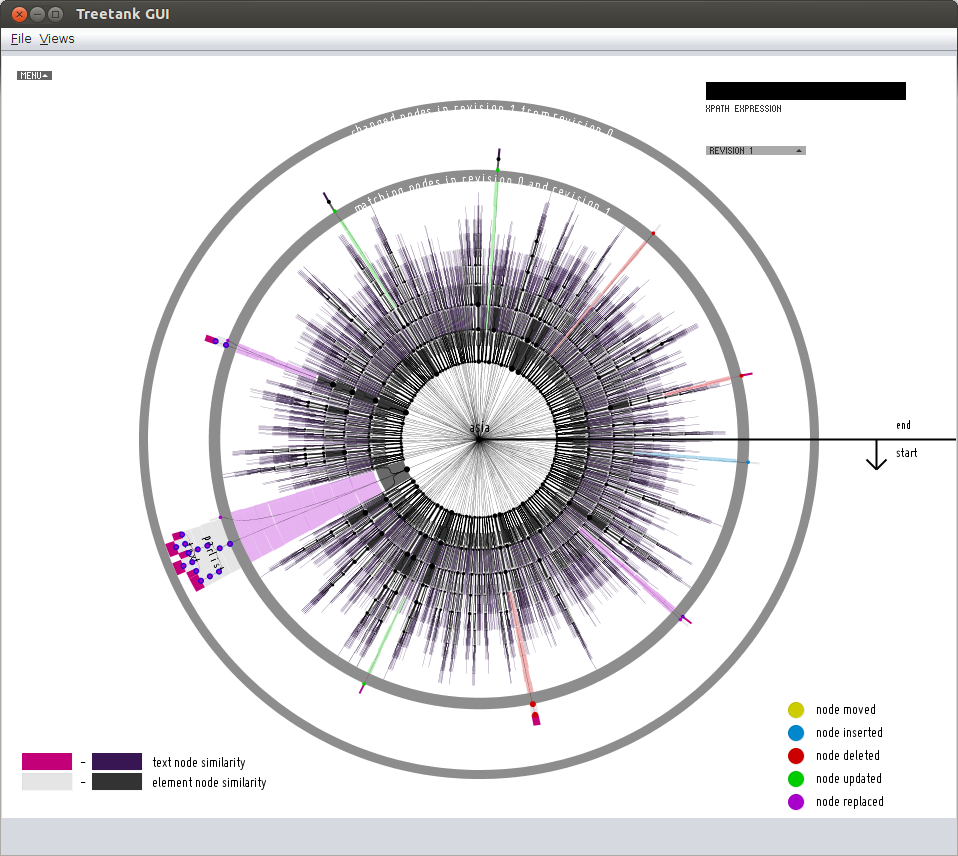
\includegraphics[width=\textwidth]
{figures/without-pruning}}
\caption{\label{fig:without-pruning} Comparison without pruning.}
\end{figure}

\begin{itemize}
\item \emph{by itemsize} Sunburst items which have no changes in its subtree and are too thin to perceive individually or too thin to select even with the fisheye transformantion are pruned based on a predefined threshold-value. An example is depicted in Fig. \ref{fig:pruned-by-itemsize}. This type of filtering is useful wherever nodes which do not differ are of value but depicting the whole tree will not add any significant value and/or does not . It considerably speeds up the generation of the Sunburst items in large tree-structures, however it does not effect the diff-calculation. Furthermore if a new node is selected to drill down into the tree the item creation must be redone, based on the \texttt{Diff}-axis, thus no optimization which just creates new items based on the initial set with adjusted angles can be used. The \texttt{descendant-or-self}-count as well as the \texttt{modification}-count must be recalculated. 

\begin{figure}[tb]
\center{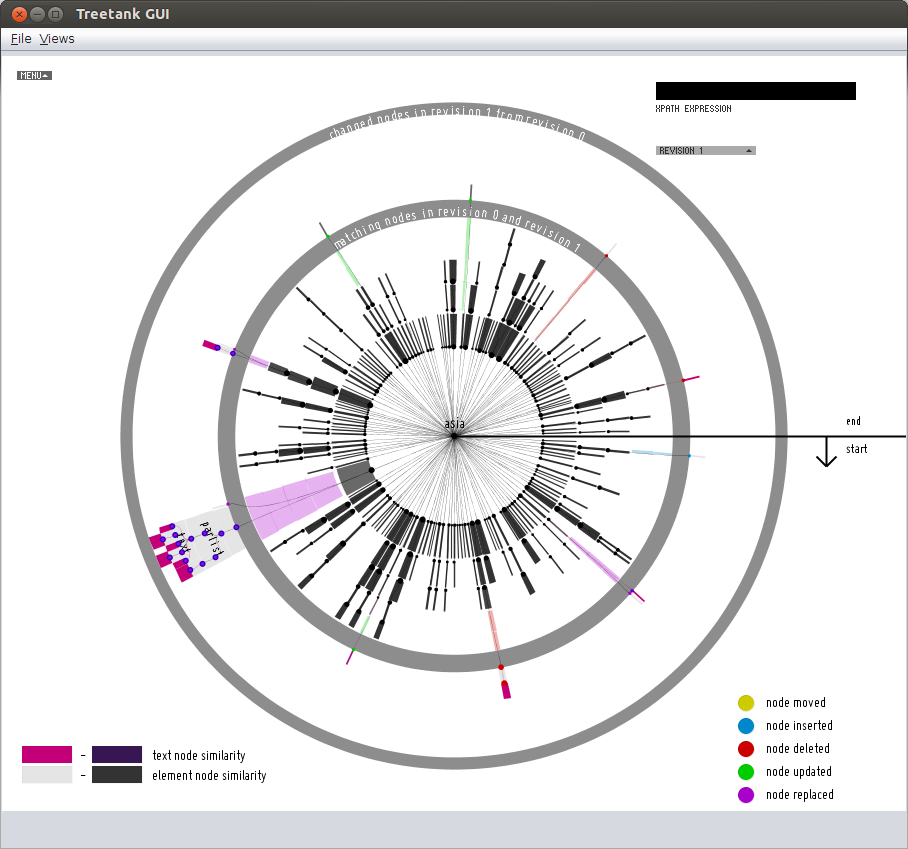
\includegraphics[width=\textwidth]
{figures/itemsize-pruned}}
\caption{\label{fig:pruned-by-itemsize} Pruned by itemsize.}
\end{figure}

\item \emph{by hash-based diff-algorithm} The diff-algorithm is called with the option to utilize persisted hashes which are created for every resource based on a database-configuration paramete. Per default rolling hashes which are very fast are used. The hashes of ancestor-nodes are recomputed for all edit-operations. As described in Chapter \ref{sec::differences} everytime the hash values during node-comparisons are identical the whole subtree is skipped in both revisions. Thus, only items are created for nodes, which contain changes in their subtree including subtree-roots for which identical hash-values are determined (Fig. \ref{fig:pruned-by-hash}). This type of pruning is especially useful for large tree-structures, whereas in contrast to the pruning by itemsize it speeds up the diff-computation as well as the item creation, as in both cases subtrees of nodes with the same hashes are skipped. However, it might be that more items in comparison with the itemsize-based approach are created as nodes with identical hash-values are always included.

\begin{figure}[tb]
\center{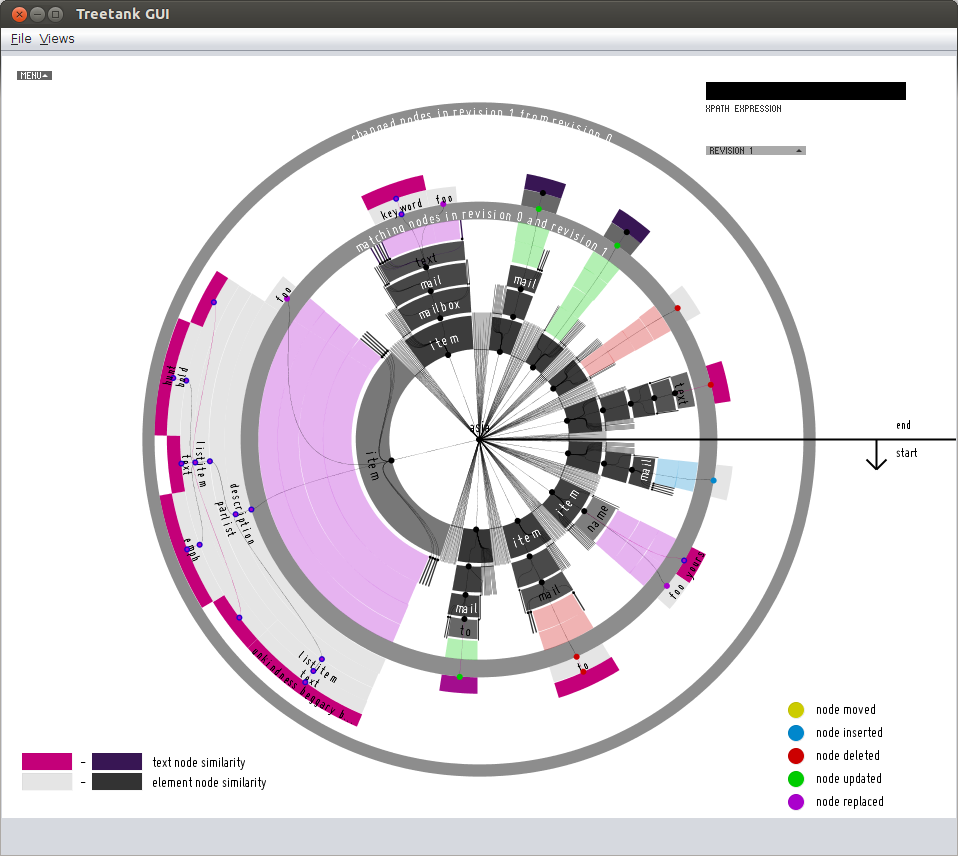
\includegraphics[width=\textwidth]
{figures/diff-pruned}}
\caption{\label{fig:pruned-by-hash} Pruned by same hashes.}
\end{figure}

\item \emph{by hash-based diff-algorithm without nodes which have the same hash} This type of pruning is closely related to the filtering-method described above. In addition to filtering nodes in the subtree of nodes which have the same hash-value, items for this type of "difference" are not created at all. A consequent is a much better readability of the differences in case of many consecutive nodes with the same hash-value (Fig. \ref{fig:pruned-by-hash-without-samehashes}).

\begin{figure}[tb]
\center{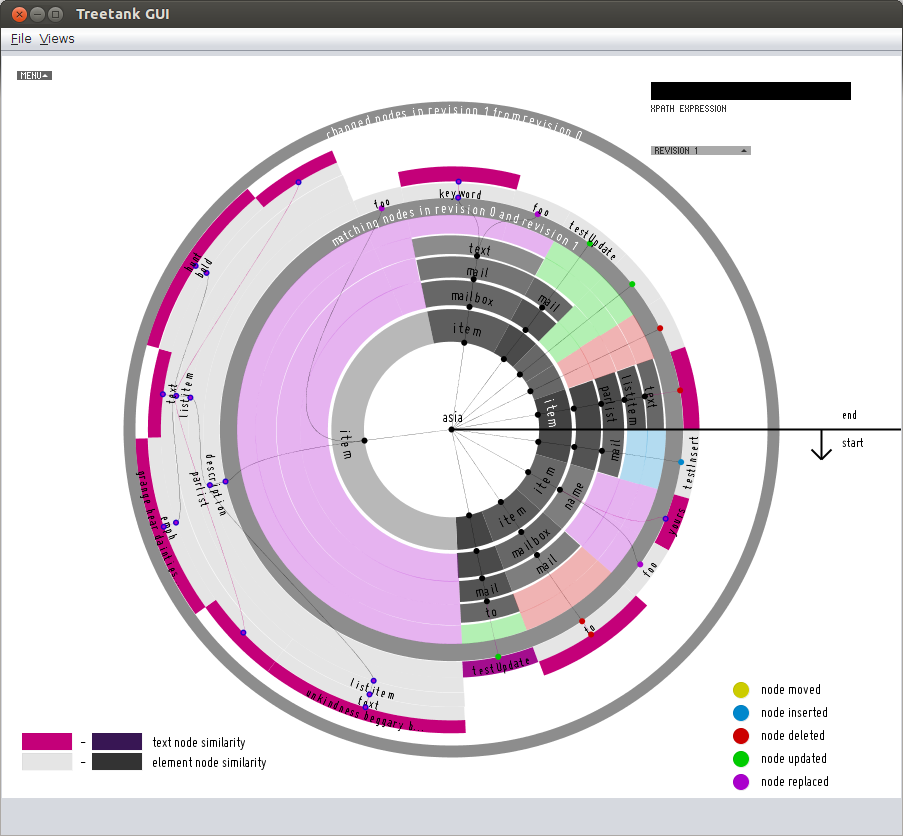
\includegraphics[width=\textwidth]
{figures/diff-without-samehashes-pruned}}
\caption{\label{fig:pruned-by-hash-without-samehashes} Pruned by hash-value without building items for nodes with same hash-values.}
\end{figure}
\end{itemize}

Usually the maximum depth of unchanged nodes in the aggregated tree-structure is computed in parallel using a \texttt{BlockingQueue} if more than two cores are available taking diff-tuples off the head of the queue during observation. However, all filtering types require postprocessing as maximum depth nodes might either be within the subtree of an unchanged node and in case of the itemsize-based filtering might be too thin regarding a threshold value. Thus, the maximum depth must be recomputed and the depth of unchanged nodes must be adapted and reduced accordingly. Note, that otherwise too much space would be wasted as the root of changed nodes is plotted at \emph{maxDepth of unchanged nodes} plus two.

Having described several filtering methods and briefly meantioned a general zooming/panning technique based on affine transformations which is inherited from the \emph{SunburstView} layout depicting one revision. Besides it is of the utmost importance to enlarge specific subtrees in the layout itself. The next section gives some insight on how to the selection of new root-nodes to dig deeper into the tree-structure is handled.

\subsubsection{Zooming / Details on demand} 
Supporting analyists with the ability to dig deeper into the tree-structure for most but the tiniest tree-structures is crucial. Thus we support the selection of a new root node by a mouse-click on the desired item. In our first version this triggered the recalculation of the diffs for the nodes' subtree as well as the the maximum depth of unchanged nodes, the modification- and the descendant-count for each node in the subtree to build new enlarged items. The former items are pushed on a stack to support a simple undo-operation.

However due to unnecessary recalculations despite in case of the item-based pruning our simplyfied approach just recalculates the maximum depth of the unchanged nodes in parallel utilizing all available cores and subsequently builds new items based on a simple upscaling.

Having described the new Sunburst-layout tailored to comparison of tree-structures with all available pruning methods and the ability to select a new root-node in detail the next section describes how the similarity score between different types of nodes is measured, which is used to map colors to the items.

\subsubsection{Similarity measures}
Similarities for \texttt{Element}- and \texttt{Text}-nodes are measured differently. The only inner nodes of an XML-document are element nodes (which can also be leaf nodes).

\texttt{Element}-node similarity is measured based on overlapping subtrees. Consider the comparison of tree-structures T1 and T2. The similarity score for an element in the aggregated tree-structure $T_{aggr}$ is defined as

\begin{equation}
Sim(node_{T_{aggr}}) = \frac{descs(node_{T_{aggr}}) - mods(node_{T_{aggr}})}{descs(node_{T_{aggr}})}
\end{equation}

The similarity score is normalized between $[0, 1]$. The nodes of type\\ \texttt{INSERTED/DELETED/REPLACED} always are scored 0 as they do not have any equivalent in the other tree. In case of \texttt{SAME}-nodes the similarity depends on overlapping subtree-structures. If no modifications are in the subtree the score is 1. \texttt{UPDATED} nodes are counted as a modifications and therefore add to the dissimilarity.

\texttt{Text}-nodes are leaf nodes which therefore have no child. The similarity score is defined as

\begin{equation}
Sim(node_{T_{aggr}}) = \left\{ \begin{array}{cl}
Levenshtein(node_{T_{1}}, node_{T_{2}}) & \textrm{if }node\ is\ \texttt{UPDATED}\\
0 & \textrm{if }node_{T_{aggr}}\ is \texttt{INSERTED}\\
  & \texttt{/DELETED/REPLACED}\\
1 & \textrm{otherwise}\end{array}\right.
\end{equation}

Note that the similarity score is computed based on the diff-tuple which incorporates both nodeKeys. In case of an \texttt{UPDATED} \texttt{text}-node the Levenshtein algorithm is used, which defines a similarity score based on per-character edit-operations to change one string-value into the other one and is normalized between 0 (no similarity) and 1 (same string-value). 

\subsection{Querying}
XPath 2.0 queries are currently partly supported by our XPath 2.0 engine. We also examined our Saxon binding, which was surprisingly rather slow. However we did not measure time differences which is out of scope of this thesis. Future work might include a Brackit\cite{Brackit} binding which is a "flexible XQuery-based query engine" developed at the TU Kaiserslautern. In contrast to Saxon it is specifically designed to work on top of databases and adding specific indexes for instance will be easy. However this feature is currently reevaluated.

We provide query capabilities on top of the agglomerated tree-structure and therefore query both compared revisions in parallel. The items are sorted by node-ID in parallel. Once all query results have been collected they are also sorted (the result is a sequence of node-IDs). A subsequent traversal of the items highlights items which are included in the query results.

\subsection{Visualization of moves}
Hierarchical Edge Bundles\cite{Bundles} are used to avoid visual clutter of subtree moves. The technique creates a path up to but usually not including the Lowest Common Ancestor (LCA) of a source-node down to the destination-node. The path is used to define control points for plotting a curve.

The LCA is defined as:

\begin{equation}
lca(a{,} b) = min\{c|a \prec c, b \prec c\}
\end{equation}

A simple algorithm computes the LCA through the \texttt{push()}-operation on two stacks following the first node (moved from) and the second node (moved to) up to the root-node. In a next step the two stacks are processed in a loop using \texttt{pop()} as long as identical node-IDs are found. The LCA is the first node-pair for which the node-IDs do not match.

Fig. \ref{fig:moves} illustrates two move-operations on a subtree in a shakespear XML-document.

\begin{figure}[tb]
\center{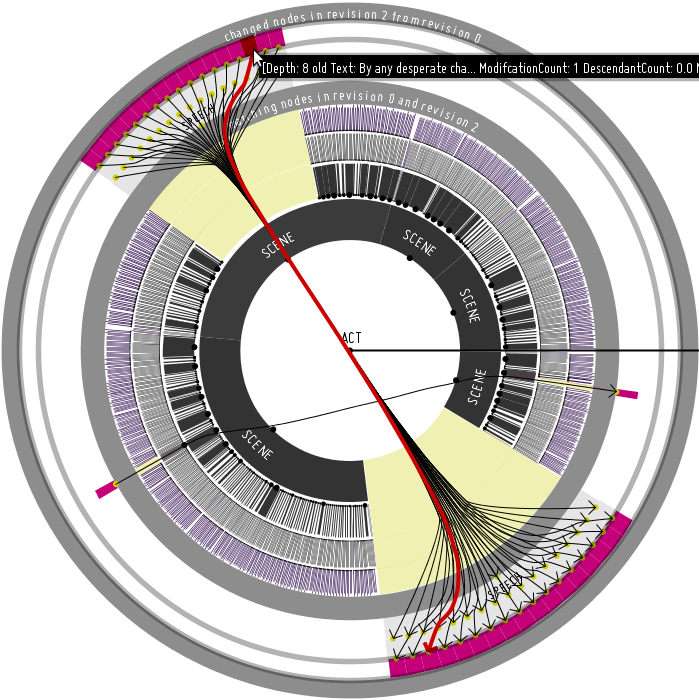
\includegraphics[width=\textwidth]
{figures/moves-cut}}
\caption{\label{fig:moves} Moves visualized using hierarchical edge bundles.}
\end{figure}

Despite comparing two tree-structures we furthermore aim to support a broad overview about the changes (and similarities) of currently at most five trees.

\subsection{Small multiple}\label{subsec::smallmultiple}
Small multiple visualizations of the \emph{SunburstView} are therefore used to provide an overview about the changes between several tree-structures, whereas the restriction of comparing five tree-structures is merely an implementation detail which in future versions will be configurable. Two variants based on same-titled well known revisioning strategies are described next.

\begin{itemize}
\item \emph{differential} The differential variant displays changes related to a base revision. This is especially useful if several tree-structures have to be compared to a common base revision. The direction is clockwise. That is the upper left corner displays a SunburstView comparison between revision 0 and 1 (if zero is the base revision which is loaded), the right upper corner displays changes between revision 0 and revision 2 et cetera (Fig. \ref{fig:smallmultiple-differential}).

\begin{figure}[tb]
\center{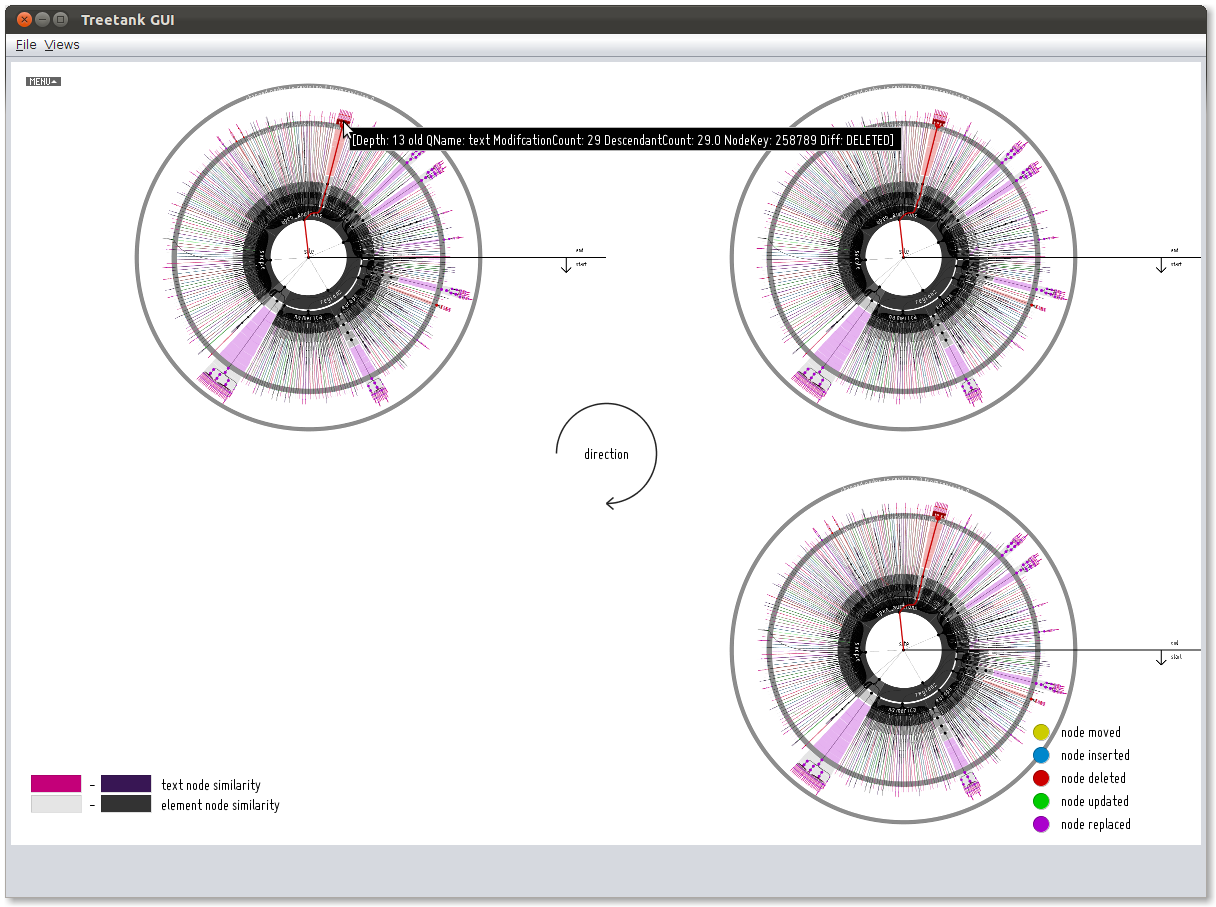
\includegraphics[width=\textwidth]
{figures/smallmultiple-differential}}
\caption{\label{fig:smallmultiple-differential} Small multiple - differential variant.}
\end{figure}

\item \emph{incremental} The incremental variant displays changes related to the last compared revision in increasing order. Suppose we have loaded revision 2, then in the upper left corner revision 2 and 3 is compared, the upper right corner contains the comparison between revision 3 and 4 et cetera (Fig. \ref{fig:smallmultiple-incremental}).

\begin{figure}[tb]
\center{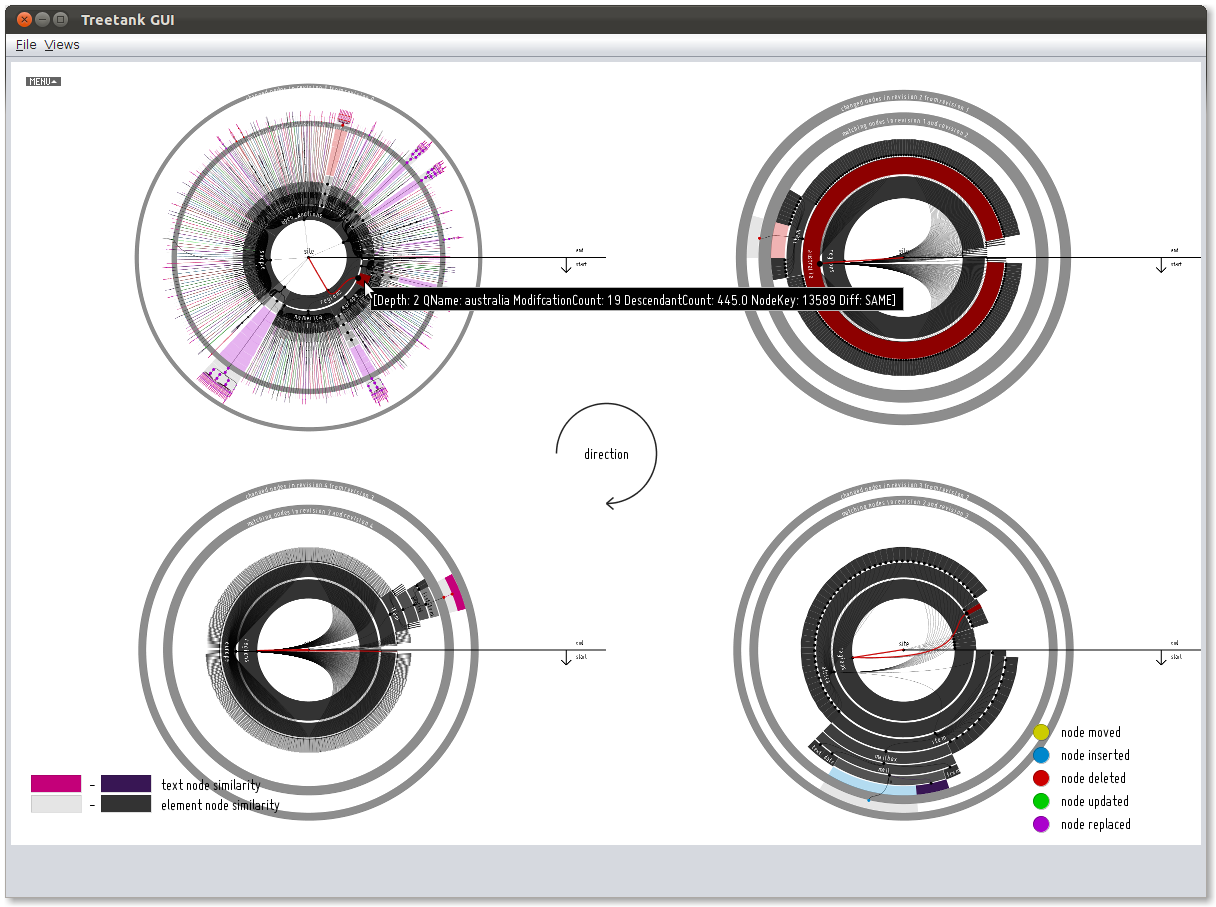
\includegraphics[width=\textwidth]
{figures/smallmultiple-incremental}}
\caption{\label{fig:smallmultiple-incremental} Small multiple - incremental variant.}
\end{figure}
\end{itemize}

The implementation parallizes the computation of the small multiple and stores each Sunburst-visualization in an offscreen image, which is appended to a list in the view. This list must be sorted after all visualizations have been computed accoring to a revision which is saved along with the buffered offscreen image to support the clockwise order. The items of each visualization are saved in a simple datastructure in the model to support highlighting of items on mouse over through brushing and linking. The technique is illustrated in Fig. \ref{fig:smallmultiple-differential} and \ref{fig:smallmultiple-incremental}. Items are highlighted in red just like in the SunburstView but the same item based on a node-ID equivalence relation is linked and highlighted in all small visualizations.

The three variants support all filtering methods described earlier. However in the case of the hybrid view only the itemsize-based pruning is of any value. Otherwise most items would not be plotted in subsequent revisions.

Next we provide a short asymptotic runtime- and space-analysis backed by performance measures.

\subsection{Runtime/Space analysis and scalability of the ID-based diff}
The runtime of the algorithm currently is bound by determining the number of descendants and modifications in the agglomerated tree-structure for each node. The runtime complexity thus is $O(n^2)$ whereas $n$ is the sum of changed and unchanged nodes between two trees $T1$ and $T2$. However by storing the diff-tuples which only include the depth of the two compared nodes to form a very simple tree-structure we are limited to a preorder traversal. Building a more sophisticated tree-structure based on pointers or sequences denoting child nodes for instance in an in-memory Treetank structure will support a subsequent postorder traversal to determine the number of descendants and modifications for each node reducing the runtime to $O(n)$. Due to using Java7 which is not available for OS X we were not able to measure the performance on computers with four or more cores. However, counting the subtree-size and modifications is started in parallel to building Sunburst items which consumes these through a Java \texttt{BlockingQueue}. The \texttt{descendant-count/subtree-size} of the root-item (plus one) is the size of the accumulated List or Map of diff-tuples observed from the ID-based diffing algorithm and thus does not need to be computed. The \texttt{modification-count} of the root-item is also determined on the fly while observing diff-tuples. Thus we assume adding more cores will speed up the creation of the items considerably as tree-structures often times are rather flat and have a large fan-out instead of being deep with high average levels/depths of the nodes, especially considering document-centric XML \cite{ronnau2009efficient}. Fig. \ref{fig:gui-performance} shows performance measures, the average of ten runs of the Sunburst-visualization on an 11MiB-document and an 111MiB-document of the XMark-benchmark.  The documents are identical to the documents used in Chapter \ref{sec::differences} for benchmarking. Thus we randomly modified the instances after every 1000st node in the 11Mib-document and after every 10000st node in the 111MiB-document. The hardware used is also identical (Core 2 Duo 2666Mhz, 4Gb RAM). It is obvious that the exponential growth in case no pruning is enabled is unacceptable. Showing the 111MiB-document without pruning lasted too long (> 15min for each run) such that we aborted the execution. By reducing the number of Sunburst-items which have to be created considerably each one of the pruning-mechanisms reduces the runtime tremendously. Usually the number of Sunburst-items to create is reduced so much that the exponential time to compute the modifications in each nodes' subtree plus the subtree-size itself is not measurable and the runtime reduces to a linear scale. Furthermore as we were not able to measure the impact of parallelizing this task with four and more cores it might also considerably speed up the computation in the general case without pruning. We assume that the context switches with only one or two cores in fact slow down the computation. 

Fig \ref{fig:gui-performance-movedet} shows benchmarking results comparing the runtime of the fastest pruning, pruning-by-hashes without creating items for identical hashes with move-detection enabled and disabled. We are able to determine that the move-detection usually is fast. Asymptotically it is bound by the size of the agglomerated tree-structure $n$, $O(n)$.

In summary we are able to conclude that the hash-based-pruning without creating Sunburst items is by far the fastest and that the move-detection usually does not inhibit the runtime of our algorithms considerably. Furthermore it is required to use pruning whenever the exponential time required to compute subtree-sizes and modifications therein significantly inreases due to a large aggregated tree. Adding more CPUs however should decrease the runtime as the computation of subtreesizes and modifications therein are computed in parallel.

\begin{figure}[tb]
\center{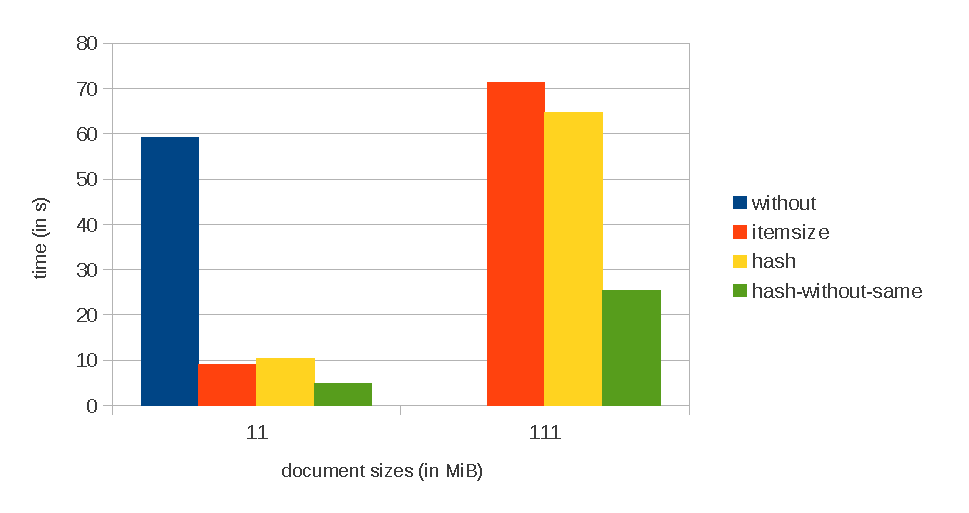
\includegraphics[width=\textwidth]
{figures/gui-performance}}
\caption{\label{fig:gui-performance} GUI-performance.}
\end{figure}

\begin{figure}[tb]
\center{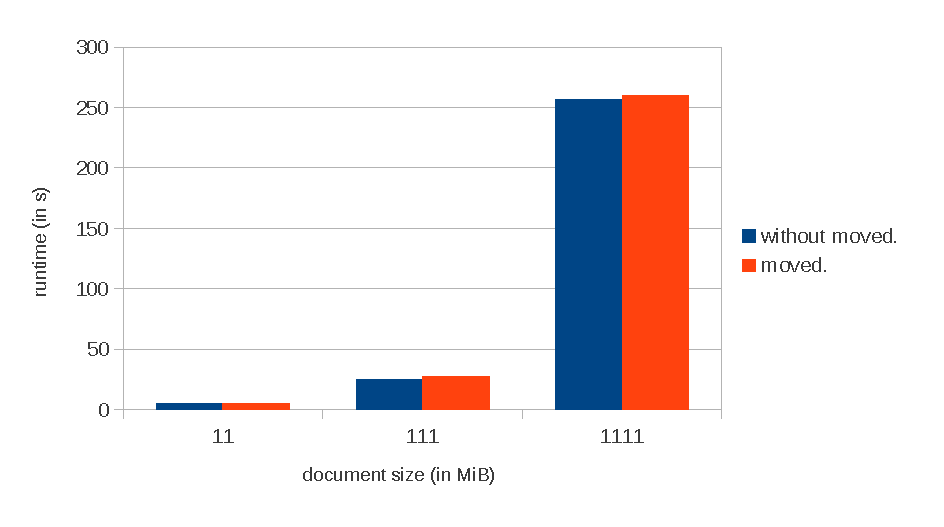
\includegraphics[width=\textwidth]
{figures/gui-performance-movedet}}
\caption{\label{fig:gui-performance-movedet} GUI-performance using hash-based pruning without adding identical hash-values and move-detection enabled/disabled.}
\end{figure}

\begin{table}[tb]
\centering 
\begin{tabular}[r]{|l|c|c|c|} 
\hline
& \textbf{1000mods} & \textbf{5000mods} & \textbf{10000mods}\\
\hline
\hline
\textbf{min} & 36265.14 & 35717.34 & 33948.96\\
\hline
\textbf{max} & 52459.38 & 61860.29 & 44451.06\\
\hline
\textbf{average} & 39167.75 & 37650.67 & 36579.37\\
\hline
\end{tabular}
\label{chap3:comparsion}
\vspace{0.5em} 
\caption{Comparsion of different modification-schemas of a 111 MiB XMark instance (change every 1000st, 5000st and 10000st node).}
\end{table}

\subsection{Conclusion and Summary}
We have introduced a multitude of visualizations ranging from a simple \emph{TextView} displaying syntax highlighted serialized XML in the viewport and appends new text during scrolling to a \emph{SunburstView} and several \emph{Smallmultiple} variants based on the \emph{SunburstView}. Our main contribution is a new Sunburst layout based on the idea of a semantic zoom, which places all changed nodes prominently between two rings and distorts the whole layout to enlarge subtrees which include changed nodes and to shrink whole subtrees with no changes. 

Moreover three filtering techniques have been described which especially facilitate the analysis of large tree-structures. Pruning by itemsize is useful if changed \emph{and} and unchanged nodes are of importance speeding up the creation of items considerably. However it does not affect the diff-computation. Thus, we introduced hash-based filtering techniques, which utilize the diff-algorithm with the optimization to skip the traversal of subtrees of nodes with same hash-values. These filtering types reduce the number of items even more. Additionaly the diff-computation is faster due to the optimization. Note that changed nodes are never skipped and therefore only nodes of no or less interest are lost and not displayed.

Move-detection is enabled on demand. Furthermore inserted/deleted subtrees in a row are summarized as replace-operations.

In addition to the \emph{TextView} and \emph{SunburstView} small multiple variants support the comparison of multiple trees ($> 2$). The number of comparsions is only limited by our implementation (which is only an implementation-detail) and the available screen space. Note, that the small multiples currently use too much unused screen space due to storing the whole visualization except the legends and menus in an offscreen image. As the with of the main GUI-window usually is not squarified the space used for menu-components and legends in the \emph{SunburstView} is multiplied and wasted. However this is merely an implementation detail which will be fixed in a future version. The filtering techniques are also available. In case of severe variations of the number of differences the incremental variant benefits the most.









\cleardoublepage
\section{Applications}\label{sec::applications}
\subsection{Introduction}
The last chapters described in detail the different components involved in our Visual Analytics approach for comparing tree-structures. This chapter exemplary studies three usage scenarios and describes additional preprocessing steps if necessary. To demonstrate the feasability of our approach with real world data the following three applications are studied:

\begin{itemize}
\item Import of Lexical Functional Grammar (LFG) XML exported files.
\item Import of sorted Wikipedia articles by revision-timestamps. 
\item A Directory recursively watched for changes within a filesystem. The XML representation thereof is based on FSML\cite{FSML}. 
\end{itemize}

\subsection{LFG}
Linguists often face the problem of having to compare Abstract Syntax Trees (ASTs). The LFG (Lexical functional grammar) in particular differenciates between two structures:

\begin{enumerate}
\item{Constituent structures (c-structures)} which "have the form of context-free phrase structure trees".
\item{Functional structures (f-structures)} "are sets of pairs of attributes and values; attributes may be features, such as tense and gender, or functions, such as subject and object."\cite{LFG}
\end{enumerate}

We obtained an XML-export of a collection of different versions of a c-structure/f-structure combination. To import differences between these XML documents in Treetank the FMSE-algorithm described in Chapter \ref{sec::relwork} and \ref{sec::differences} is used for the simple reason that the XML-export does not include unique node identifiers. Thus we can not rely on node-IDs and have to figure out differences using our similarity metrics defined for leaf- and inner-nodes. Fig. \ref{fig:lfg} illustrates the visualization of a diff between two revisions.

\begin{figure}[tb]
\center{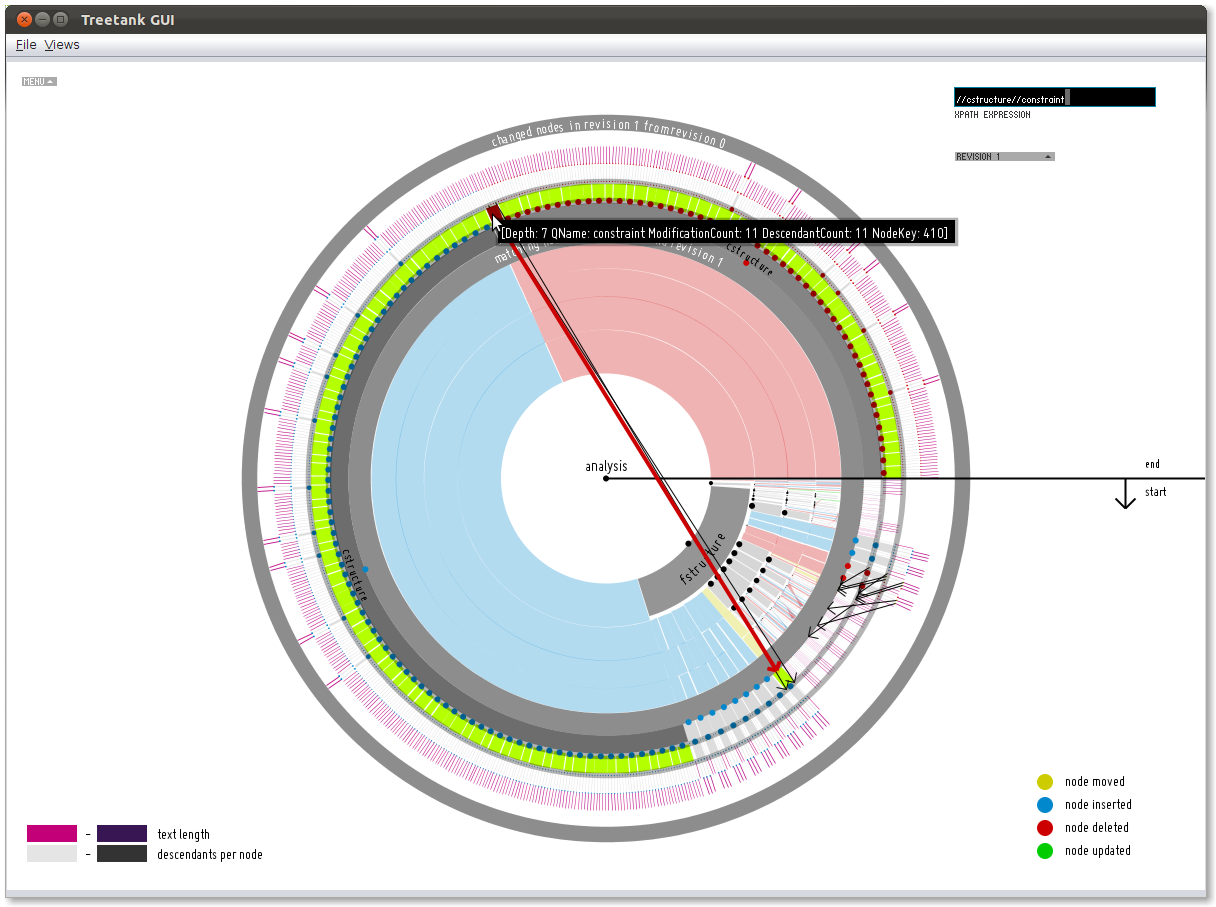
\includegraphics[width=\textwidth]
{figures/lfg.png}}
\caption{\label{fig:lfg} LFG comparsion.}
\end{figure}

It is immediately obvious by investigating the original XML-documents, that the FMSE-algorithm mismatched nodes in the first place which in effect causes a lot of edit-operations. Nodes are touched which are not changed and vice versa\footnote{note, that the final outcome is nontheless correct in terms of the first tree-structure is correctly edited to represent the second}. Thus, the FMSE-algorithm does not generate a minimum edit-script and executes too many edit-operations especially in case of the deletion and reinsertion of the old- respectively the new-\texttt{cstructure} subtree. In doing so, a subsequent visualization is impractical, for the simple reason that it almost mirrors the update-operations issued by the FMSE-algorithm for consecutive versions. As stated in Chapter \ref{sec::relwork} ID-less algorithms work best if leaf nodes and therefore especially text-nodes are very well distinguishable. That is the initial matching of leaf nodes in most if not all cases really matches unchanged nodes, which is the desired behavior. 

Having a close look at the input documents reveals a lot of changed or updated text-values (Listing \ref{lst:linguistscomparsion}). Our threshold value for matching subtrees in case of inner nodes is $0.5$ (has to be $> 0.5$ for matching nodes) and thus the arg-elements are not matched.

For that reason we changed the leaf-node comparison slightly. Instead of just relying on the Levenshtein-distance for text-node values we also try to match all ancestor \texttt{QName}s \footnote{ancestors are always element nodes, the document-root node is not visited} if the returned normalized value is $<=$ the threshold value defined for the similarity of leaf nodes. Note that only leaf nodes are considered to match if the threshold is $>$ than the predefined threshold. Hence, the leaf nodes are matched and "updated" by FMSE instead of deleting/inserting the whole subtree.

The result is depicted in Fig. \ref{fig:linguistics}.

However as a direct consequence of this short evaluation it is inevitable to rely on unique node identifiers if we want to visualize minimal edit-scripts in case of updated leaf node values which are very distinct to the other trees' leaf node values or worse the leaf nodes are very similar. Comparisons based on similarity-metrics are always based on heuristics. Assuming the export of the XML-documents includes unique identifiers of the nodes, importing requires utilization of the internal diff-algorithm to simply store incremental changes, the changes from the old- to the new-revision. The following steps have to be implemented:

\begin{enumerate}
\item Import of the initial XML-document.
\item Import the first updated XML-document to a temporary resource.
\item Utilize the internal Treetank diff-algorithm to determine changes based on unique node-IDs. Whenever an edit-operation is encountered the appropriate transaction-method has to be executed. %In case of \texttt{element}- and \texttt{text}-nodes it requires how to insert nodes\footnote{remember that Treetank currently is able to insert a node as a right sibling or first child} and where, which is very simple due to the \texttt{transaction.moveTo(long)}-method which can move the transaction/cursor directly to the left-sibling-node of the node to insert if it is available or to the parent. In the first case the node has to be inserted as a right sibling, in the latter case as a first child of the parent node.
\end{enumerate}

\begin{figure}[tb]
\center{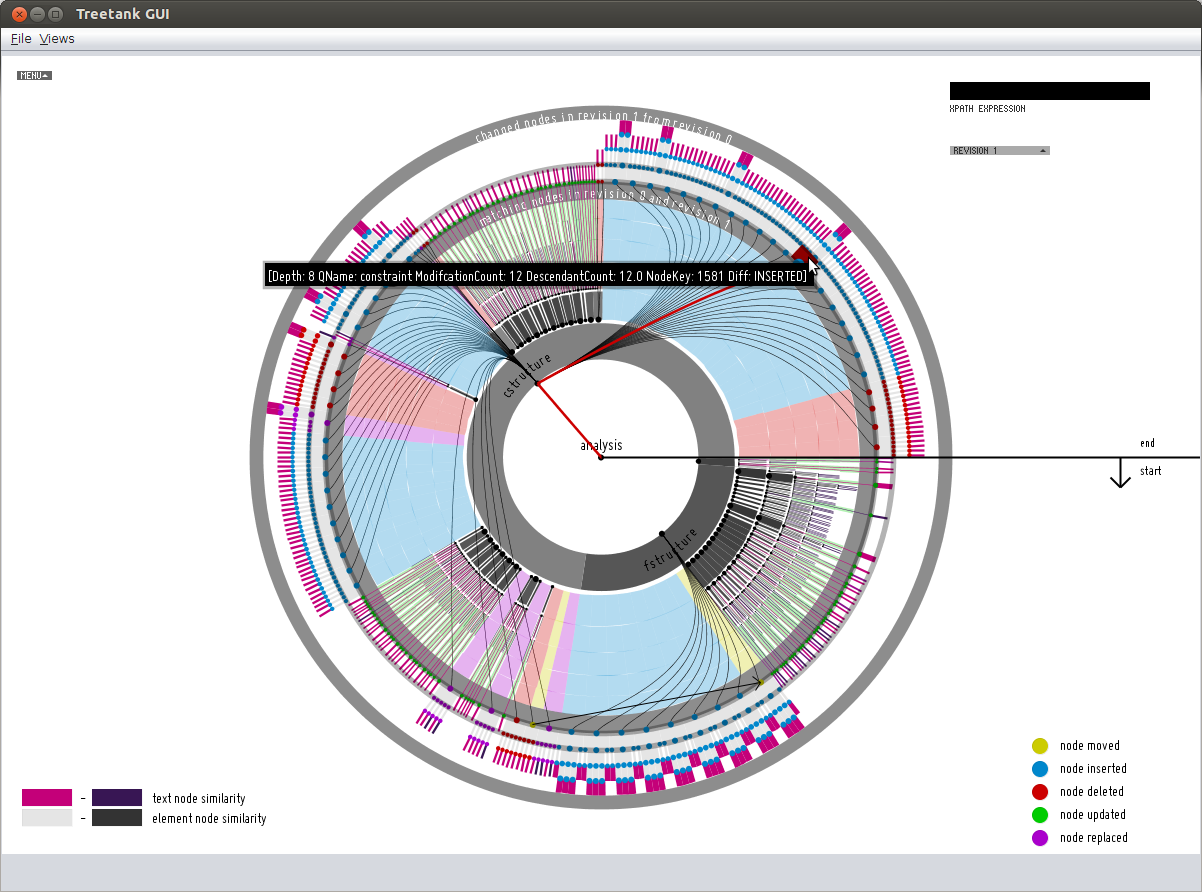
\includegraphics[width=\textwidth]
{figures/linguistics.png}}
\caption{\label{fig:linguistics} LFG comparsion revised.}
\end{figure}

We observe that still many nodes are changed, but by looking at the original XML-documents we observe that indeed a lot of nodes have been updated/deleted/inserted or replaced. For instance by scrolling both XML-documents at the end of the fstructure-subtree a lot of subtrees must have been inserted.

\begin{code}[caption=CStructure/FStructure comparsion]
<cstructure>                   <cstructure>
  <constraint>                   <constraint>
    <label>subtree</label>         <label>subtree</label>
    <arg no="1">102</arg>          <arg no="1">163</arg>
    <arg no="2">ROOT</arg>         <arg no="2">ROOT</arg>   
    <arg no="3">-</arg>            <arg no="3">-</arg>
    <arg no="4">83</arg>           <arg no="4">145</arg>
  </constraint>                  </constraint>
  <constraint>                   <constraint>
    <label>phi</label>             <label>phi</label>
    <arg no="1">102</arg>          <arg no="1">163</arg>
    <arg no="2">var:0</arg>        <arg no="2">var:0</arg>
  </constraint>                  </constraint>
  ...                            ...
</cstructure>                  </cstructure>
\end{code}
\label{lst:linguistscomparsion}

Furthermore this approach applies to every XML-document which incorporates unique node identifiers.

Next, we study the import of several articles from Wikipedia ordered by timestamp of their revisions. 

\subsection{Wikipedia}
Wikipedia is studied as an application to demonstrate the feasability of our approach on a large text corpora. However several issues have to be solved during preprocessing.

\begin{itemize}
\item Wikipedia is dumped as a very large XML-file. "'The XML itself contains complete, raw text of every revision"'\cite{WikiDump} and thus is a full dump instead of an incremental- or differential-dump describing the changes an author performed. Appendix \ref{sec::wikidump} depicts a small example of the structure of an Wikipedia XML-dump. Moreover WikiText, which is a proprietary markup format is stored as plain text and not replaced by XML-markup. Thus, the content of an article in each revision is a huge \texttt{TextNode} which includes the full text instead of just denoting the changes and its context in some form. Differences between the actual content of several revisions of an article on a node-granular level can not be found with a state of the art native XML database system, which supports revisioning of the data, as a direct consequence. The database systems' best bet is to generate a character based delta between the two large text-nodes.

\item Furthermore due to the fact that XPath 2.0 should be usable without requiring an XQuery/XPath Full Text 1.0 implementation and our overall goal is to analyse the temporal evolution of the stored data, WikiText markup has to be converted into semistructured XML fragments. To accomplish this the Wiki2XML parser from the MODIS team \cite{Wiki2XML} is used.

\item Another issue arises because the Wikipedia dump is not sorted and we want to analyse and visualize the temporal evolution during several snapshots. Neither articles are sorted by date/time nor revisions of the articles are. Thus for the subsequent revisioned import the revisions have to be sorted with their associated article metadata (page id, author...). For the simple reason that we have to deal with large amounts of data an external sorting algorithm has to be used. Instead of implementing an own approach, Hadoop is a natural choice. Its \emph{MapReduce}\cite{Hadoop} framework is a "programming model and software framework for writing applications that rapidly process vast amounts of data in parallel on large clusters of compute nodes". The overall process of the programming model is divided into two functions.
\end{itemize}

\begin{enumerate}
\item \texttt{Map} is a function that splits the problem into subproblems are distributed among worker nodes in a cluster. Logically it is a function of the form \texttt{$Map(k1,v1) \rightarrow list(k2,v2)$} where $k1$ and $v1$ is an input $key$ and $value$ and the output from the function is a list of $key/value$ pairs (\texttt{list(k2, v2)}). After that the MapReduce framework groups the values according to the keys.
\item \texttt{Reduce} is a function of the form: \texttt{$Reduce(k2, list (v2)) \rightarrow list(v3)$}. It receives a $key$ and a list of grouped $values$ and performs any computation which might be feasable and returns another list of $values$.
\end{enumerate}

The \texttt{map}-function receives input data splitted into records. Most MapReduce frameworks rely on a programmable mechanism to do this. In Hadoop it is the responsibility of the \texttt{InputStream} in conjunction with a \texttt{RecordReader}. The following steps describe the implementation of sorting Wikipedia by Hadoop.

\begin{enumerate}
\item \texttt{XMLInputStream} in conjunction with an \texttt{XMLRecordReader} splits records on \emph{revision-elements} with the \emph{page}-metadata prepended. The \textbf{timestamp} of each revision denotes the key, the whole subtree of each \emph{revision}-element is saved as the value for the \texttt{map} input. The algorithm is straight forward. A \texttt{SAX-Parser} is used to determine starting and ending of each record.

The implementation utilizes a configurable record identifier such that it is adjustable to schema changes in the Wikipedia dump. 

\item \texttt{XMLMap} just forwards the received key/value pairs.
\item \texttt{XMLReduce} finally merges consecutive revisions with the same \emph{page-id} and \textbf{timestamp} by means of Saxon, an XSLT/XQuery-processor. Our XSLT stylesheet to achieve the concatenation is small yet maybe not straight forward (Appendix \ref{sec::xslt}).
\end{enumerate}

% import of wikipedia
Once the dump is sorted with MapReduce it has to be imported into Treetank. First of all, as we have splitted the data on \texttt{revision}-elements and pre\-pen\-ded the \texttt{page-}metadata we have to construct a new root node, which is simply done by prepending a \texttt{mediawiki} start-tag, then writing the result of the Hadoop-run and appending a corresponding end-tag to a new file. Otherwise it is no valid XML-document and can not be parsed by XML-parsers.

\begin{figure}[tb]
\center{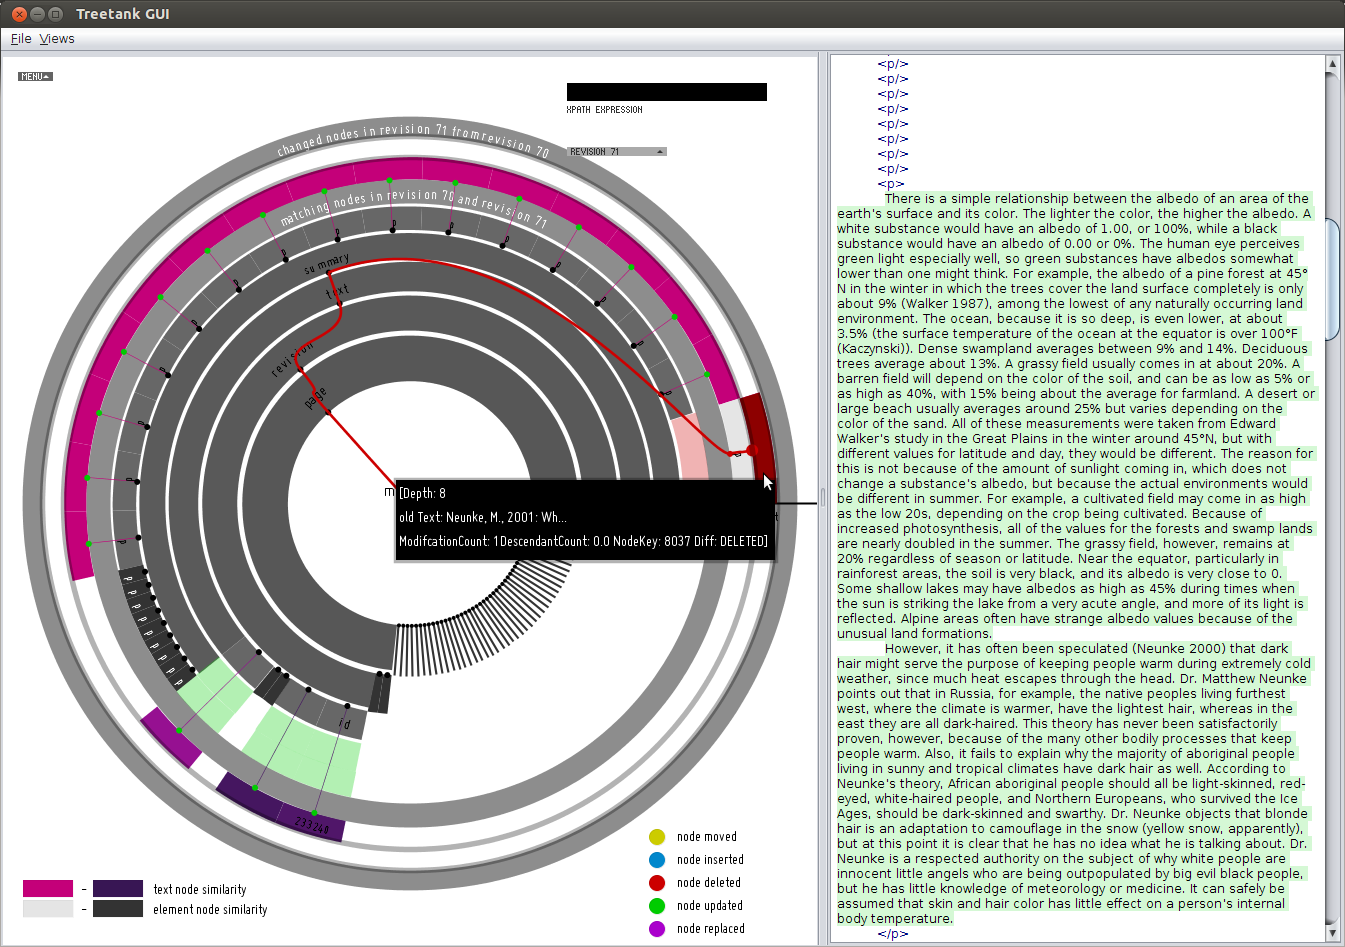
\includegraphics[width=\textwidth]
{figures/wikipedia-rev7071}}
\caption{\label{fig:wikivis} Wikipedia comparsion.}
\end{figure}

Next, it is the responsibility of a Wikipedia-Importer to import the revisioned file which is now in ascending timestamp order of all revisions from all pages/articles. It utilizes the FSME-implementation described in detail in Chapter \ref{sec::relwork} and \ref{sec::differences} to just import incremental changes between the latest stored revision in Treetank and a shredded List of \texttt{XMLEvent}s in a temporary database/resource. Therefore as data is read-in from the XML document with a StAX-Parser the page-metadata as well as the whole revision-subtree is saved in a simple main-memory collection, a \texttt{List}, assuming the XML-content of an article can be put in main memory. The assumption holds true as every revision can be parsed and rendered in a web-browser. Everytime a \texttt{page} end-tag is encountered the page-id is searched in the already shreddered revision. If it is found the FMSE algorithm is called for the found \texttt{page}-element, such that the encountered differences are shreddered subsequently. In case the XPath expression returns no results, that is the page-ID is not found a new page is going to be appended as a right sibling to the last \texttt{page}-element.

The Importer for Wikipedia allows the usage of a timespan (hourly, daily, monthly, yearly) which is used for the revisioning. Whenever a new timestamp is encountered, which differs from the current timestamp depending on the chosen timespan the transaction is commited.

\begin{figure}[tb]
\center{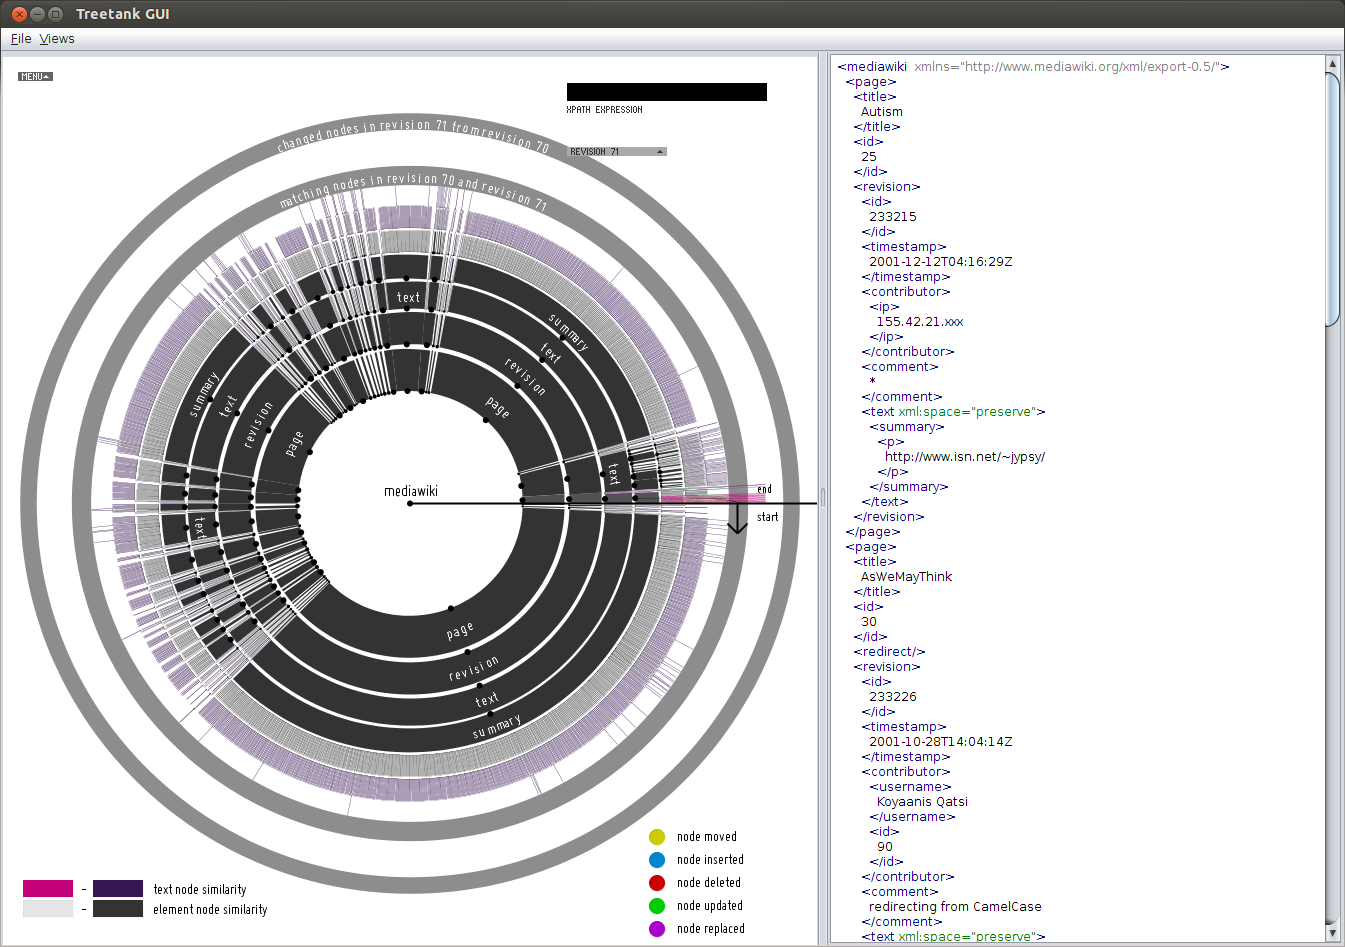
\includegraphics[width=\textwidth]
{figures/wikipedia-without-pruned-modifications}}
\caption{\label{fig:wikivis-without-modscale} Wikipedia comparsion without pruning and including the modification weight to determine the size of a SunburstItem.}
\end{figure}

Fig. \ref{fig:wikivis} demonstrates the result of importing 50 articles of Wikipedia sorted by article-revisions and an hourly commit\footnote{only hours in which changes occured are reflected}. Revisions 70 and 71 are compared. The \emph{edit-distance} used by our FSME-implementation to determine and update the stored Treetank-data with the encountered differences in the first place works reasonably well, as most text-nodes are distinguishable very well. We used the hash-based pruning to enlarge regions of interest. The \emph{TextView} on the right side is particular useful to quickly reveal several changes in particular updated text whereas a label in the \emph{SunburstView} only depicts the new updated text content in case of \texttt{TextNode} updates and usually the content is too big to be displayed within the arc, especially if the content contains whole paragraphs as is usually the case for Wikipedia. Both text values, the old- and the new-value is displayed on mouseover. We quickly detect that a lot of paragraphs have changed by looking at the \emph{SunburstView}. Details are depicted by either hovering an item or scrolling down in the \emph{TextView}. %It is fair to say, that for instance the text-nodes below the \texttt{id}-element parent could be detected as updates as well if all ancestors and neighbour nodes are checked for equality even though the Levenshtein algorithm used to compare text nodes detects too many character edit operations to consider that the nodes are equal. 

\begin{figure}[tb]
\center{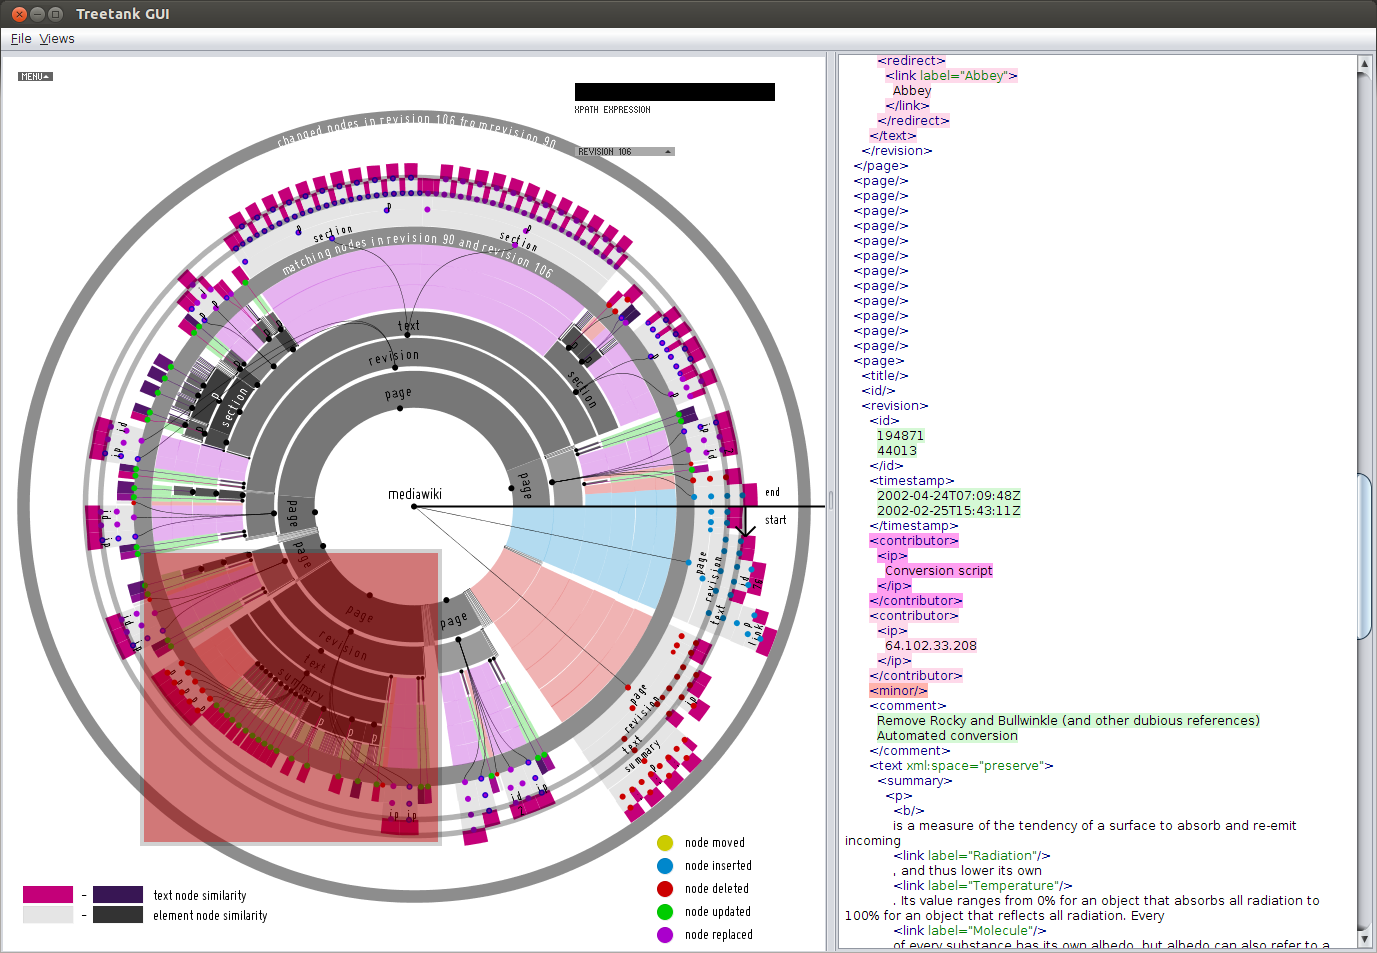
\includegraphics[width=\textwidth]
{figures/wikipedia-rev90106}}
\caption{\label{fig:wikivis-rev90106} Wikipedia comparsion pruned by itemsize.}
\end{figure}

Another visualization (Fig. \ref{fig:wikivis-without-modscale}) depicts the situation without pruning and without including the number of modifications of a node in its subtree to scale the Sunburst items, the segments for each node.

The changes in the last page/article are hardly visible. Most items denote unchanged nodes without any modifications in their subtree and thus do not carry any useful information, if we just want to quickly determine changes. This and the fact that we do not include the modification weight to scale items, that is only the subtree size of each node matters, results in considerably reduced itemsizes of changed items.

\begin{figure}[tb]
\center{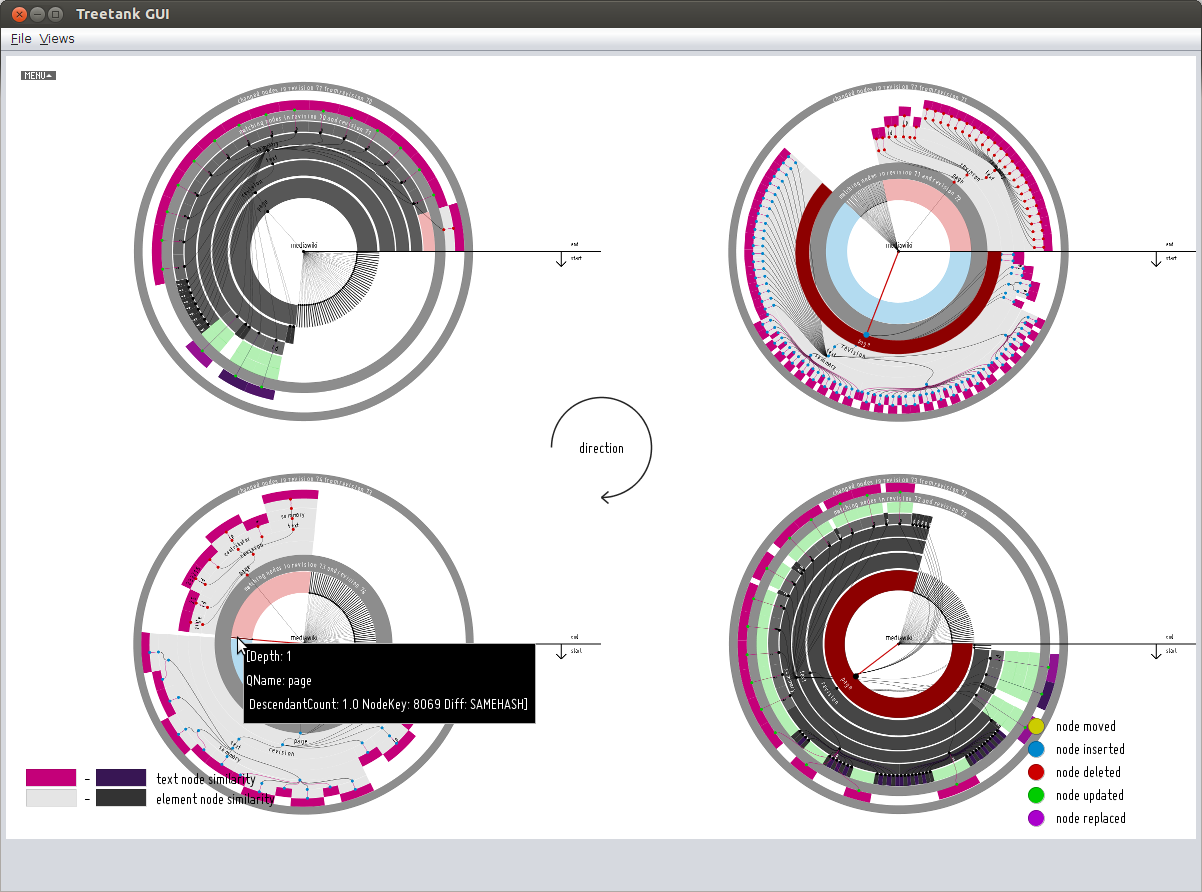
\includegraphics[width=\textwidth]
{figures/wikipedia-incremental}}
\caption{\label{fig:wikipedia-incremental} Wikipedia comparsion - depicting differences through the incremental smallmulltiple variant.}
\end{figure}

Despite viewing changes between subsequent revisions which in case of importing only 50 articles most often results in appending or updating one article it is possible to view changes between arbitrary revisions. Fig. \ref{fig:wikivis-rev90106} reveals changes between revision 90 and 106. Thus seven articles have changed and it is very easy to determine regions of interest and to further drill down into the tree through selecting a new root node in the \emph{SunburstView}. The page/article with the name "ArgumentForms" has been changed considerably. The page-nodes which are containers of the whole article do not have enough matching subtree-nodes in common between the two revisions, such that they are not matched, too. The FMSE-algorithm thus deletes the whole article and inserts the article as a new first child of the "wikimedia" root-element. The changes in the other articles mainly either include single paragraphs which are updated or larger subtrees which are replaced. Detailed changes are depicted on demand, that is if we drill down into the tree and/or scroll down in the \emph{TreeView}. The transparent red square in the \emph{SunburstView} in Fig. \ref{fig:wikivis-rev90106} illustrates the article/page to which we have scrolled in the \emph{TextView}.

Besides comparing only two revisions small multiple display variants facilitate the comparison between several revisions (currently at most five revisions). Fig. \ref{fig:wikipedia-incremental} illustrates changes between revisions 70,71 (upper left), 71,72 (upper right), 72,73 (bottom right) and 73,74 (bottom left). We are quickly able to determine that except in the SunburstView comparing revisions 73 and 74 all other small multiples change or delete/insert the same article. The comparison between revision 70,71 and 72,73 reveal a lot of updated paragraphs. Between revisions 71 and 72 the same article has been deleted and inserted. We are quickly able to determine that a lot of paragraphs have been added as the inserted article includes more descendants than the article in the old revision. Thus the FMSE-algorithm does not match the page-nodes due to very different subtrees. Repacitulate that in order to match inner nodes, more than at least half of the nodes in both subtrees have to be matched. To gain a better understanding about the differences between revision 73 and 74 we switch to the \emph{SunburstView} in conjunction with the \emph{TextView}. We are able to quickly determine that the deleted and inserted page denotes the same article (autism) once more (Fig. \ref{fig:wikipedia-rev7374}). The article changed from a single paragraph which just included a URL to a slightly more profound description of autism.

\begin{figure}[tb]
\center{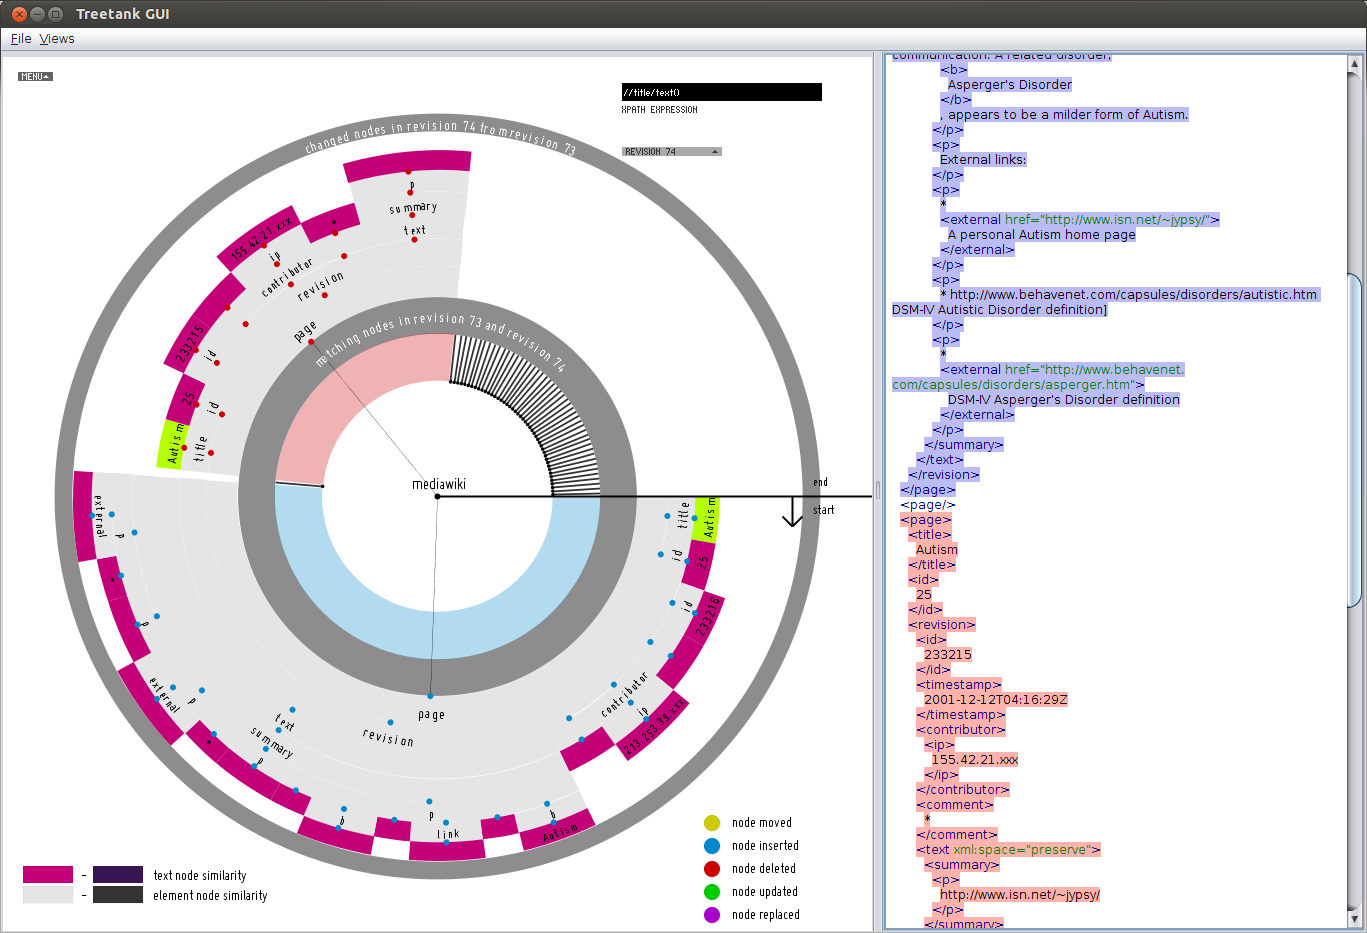
\includegraphics[width=\textwidth]
{figures/wikipedia-rev7374}}
\caption{\label{fig:wikipedia-rev7374} Wikipedia comparsion - depicting differences between revision 73 and 74.}
\end{figure}

Fig. \ref{fig:wikipedia-smallmultiple-incremental} finally reveals that between revision 10 and 13 articles are added which is expected. Articles are most probably going to be altered in later revisions once most or all 50 articles have been pre\-pen\-ded. However revision 14 updates an article added in one of the first 10 revisions.

\begin{figure}[tb]
\center{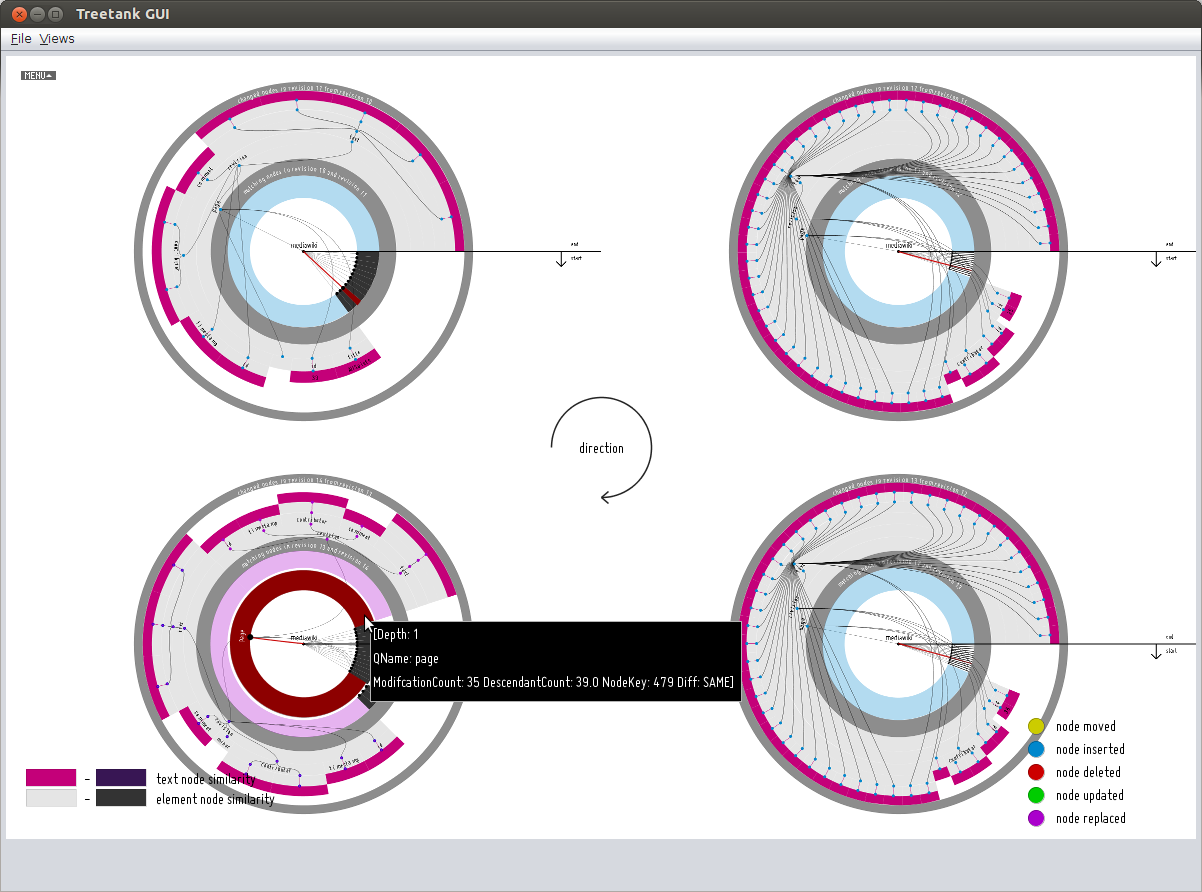
\includegraphics[width=\textwidth]
{figures/wikipedia-incremental-add}}
\caption{\label{fig:wikipedia-smallmultiple-incremental} Wikipedia comparsion - incremental smallmultiple variant depicting changes between revisions 10,11,12,13 and 14 from the upper left to the bottom left in clockwise order.}
\end{figure}

%To further emphasize the changes and to speed up the calculation we can use the pruning-mechanisms described in chapter 4. Using the pruning based on the itemsize results in Fig. \ref{fig:wikivis-pruned-itemsize}. Instead of larger itemsizes for changed nodes potentially uninteresting nodes are pruned away, which are too small and aren't modified between the two compared revisions. Note that these nodes can still be displayed as a user drills down into the tree by selecting a new root-node, whereas all subtree-nodes are scaled according to the new root.

%In order to maximally highligh nodes which are changed between the two revisions Fig. \ref{fig:wikivis-pruned-hash} displays the result of applying the hashbased diff-algorithm. Whenever same hashes are encountered for the two nodes of each revisions the whole subtree is skipped for traversal and as such also in the visualization. As a direct consequence maximal performance as well as itemsize for changed nodes is achieved. Context nodes are preserved, such that all siblings of the root-nodes regardings changes are still visible. As a matter of fact we can still enlarge the items which depict changed-nodes by tuning the variable which denotes, how much modifications are weighted in respect to the number of descedants per node in addition to the current node.

%\begin{figure}[htb]
%\center{\includegraphics[width=\textwidth]
%{figures/wikipedia-50-articles-prunedhash.png}}
%\caption{\label{fig:wikivis-pruned-hash} Wikipedia comparsion pruned by hash-comparsion}
%\end{figure}

%In order to compare sequences of revisions it's also possible to view incremental and differential changes between the loaded base-revision and the other revisions. Fig. \ref{fig:wikipedia-smallmultiples-differential} reveals the initial addition of several article, whereas the articles are not present before. In the last comparsion, the lower left SmallMultiple an article is updated instead of added. In order to zoom into interesting regions and to gain further insights the normal view comparing two revisions can be used which is going to be linked with the SmallMultiplesViews.

%\begin{figure}[htb]
%\center{\includegraphics[width=\textwidth]
%{figures/wikipedia-smallmultiples-differential.png}}
%\caption{\label{fig:wikipedia-smallmultiples-differential} Wikipedia comparsion (differential smallmultiples view)}
%\end{figure}

%Another view (Fig. \ref{fig:wikipedia-smallmultiples-hybrid}) displays the evolution whereas revision 0 is the base revision with just one article added. Afterwards other articles are appended as long as no article has been updated. Articles which haven't change within the two compared revisions are blackened.

%\begin{figure}[htb]
%\center{\includegraphics[width=\textwidth]
%{figures/wikipedia-smallmultiples-hybrid.png}}
%\caption{\label{fig:wikipedia-smallmultiples-hybrid} Wikipedia comparsion (hybrid smallmultiples view)}
%\end{figure}

\subsection{Import of Filesystem-based tree-structure}
Filesystems usually organize data in a tree-structured hierarchy whereas a unique \emph{Path} denotes the location of a file. As a direct consequence it is an optimal use case to demonstrate the feasability of our proposed approach as the tree-structure can not be neglected if we quickly want to detect differences in the folder/file-structure based on snapshots.

Use cases are manyfold, ranging from monitoring software-evolution based on the package/class hierarchy to monitoring if employees stick to organizational policies.

In order to take snapshots of a directory with all subdirectories we study two approachs:

\begin{enumerate}
\item FSML representation based on a python script \cite{FSML}, which is executed several times to obtain snapshots based on an XML-representation which are afterwards imported in Treetank. The differences between the snapshots are calculated based on the FMSE-algorithm described in Chapter 2 and 3.
\item FSML representation based on an initial import of a directory with all its subdirectories. Changes in that directory and all subdirectories are afterwards monitored.
\end{enumerate}

The File System Markup Language\cite{FSML} is an XML-dialect developed by Alexander Holupirek to represent the tree-structure of filesystems by folders and files as well as metadata of certain file-types. 

The first approach is considerably simpler than the import of Wikipedia due to the snapshot-creation which results in different files. Therefore we do not have to reorder whole subtrees according to timestamps in the first place to obtain a subsequent import ordered by time. Instead applying the FMSE-algorithm on the last imported revision and the new XML document is sufficient.

Fig. \ref{fig:fsml-gui} reveals the differences between revision 0 and 4 using the hash-based pruning on manually taken snapshots of the src-folder of our GUI project (slightly outdated) with a Python-script, developed by Alexander Holupirek, too. We are able to detect possible hotspots of development on the package/class-level. It is immediately obvious that a ForkJoin-Quicksort implementation has been deleted recently. Another interesting observation is the recent work on BSplines which have been added to facilitate the Hierarchical Edge Bundling technique described in Chapter \ref{sec::visualizations}. Furthermore we are able to spot recent work on a new \emph{Treemap}-view. The XPath-query \texttt{//element()[@st\_mode="0100664"]} highlights nodes whith the appropriate mode.

\begin{figure}[tb]
\center{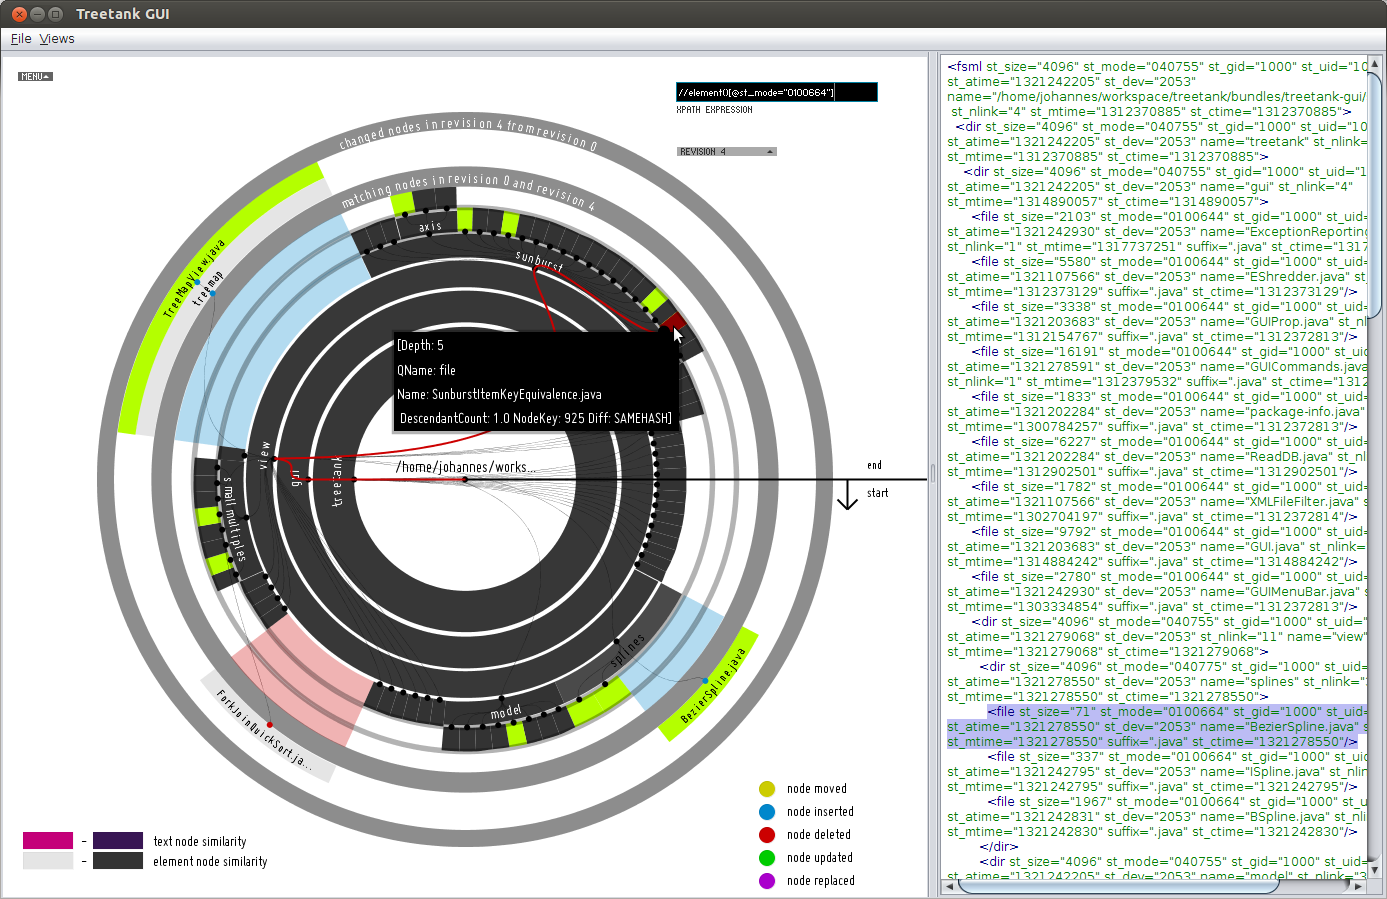
\includegraphics[width=\textwidth]
{figures/fsml-gui}}
\caption{\label{fig:fsml-gui} FSML comparsion of the GUI src-folder.}
\end{figure}

The alert reader might think that some of the nodes for instance the subtree of the "sunburst"-subtree which are plotted should not have been processed by the ID-based diff algorithm because we are utilizing the hash-based diffing algorithm, but by close inspection it is revealed that these nodes have different hash values (on mouseover the details are revealed, that is type \texttt{DiffType.SAME} instead of \texttt{DiffType.SAMEHASH}). We currently do not color-encode nodes which have identical hash-values differently to nodes with identical node-IDs but different hash-values. Moreover up until now we have always used the ID-based diffing mode which does not include namespace/attribute comparisons. However, once including checks for namespace/attribute equivalence we are able to detect updates of certain nodes (Fig. \ref{fig:fsml-gui-fulldiff}) due to last access time of a file/directory which is denoted through the \texttt{st\_atime}-attribute. Each time either a namespace- or an attribute-node differs the parent \texttt{ElementNode} is emitted as being updated once the full diff mode is enabled.

\begin{figure}[tb]
\center{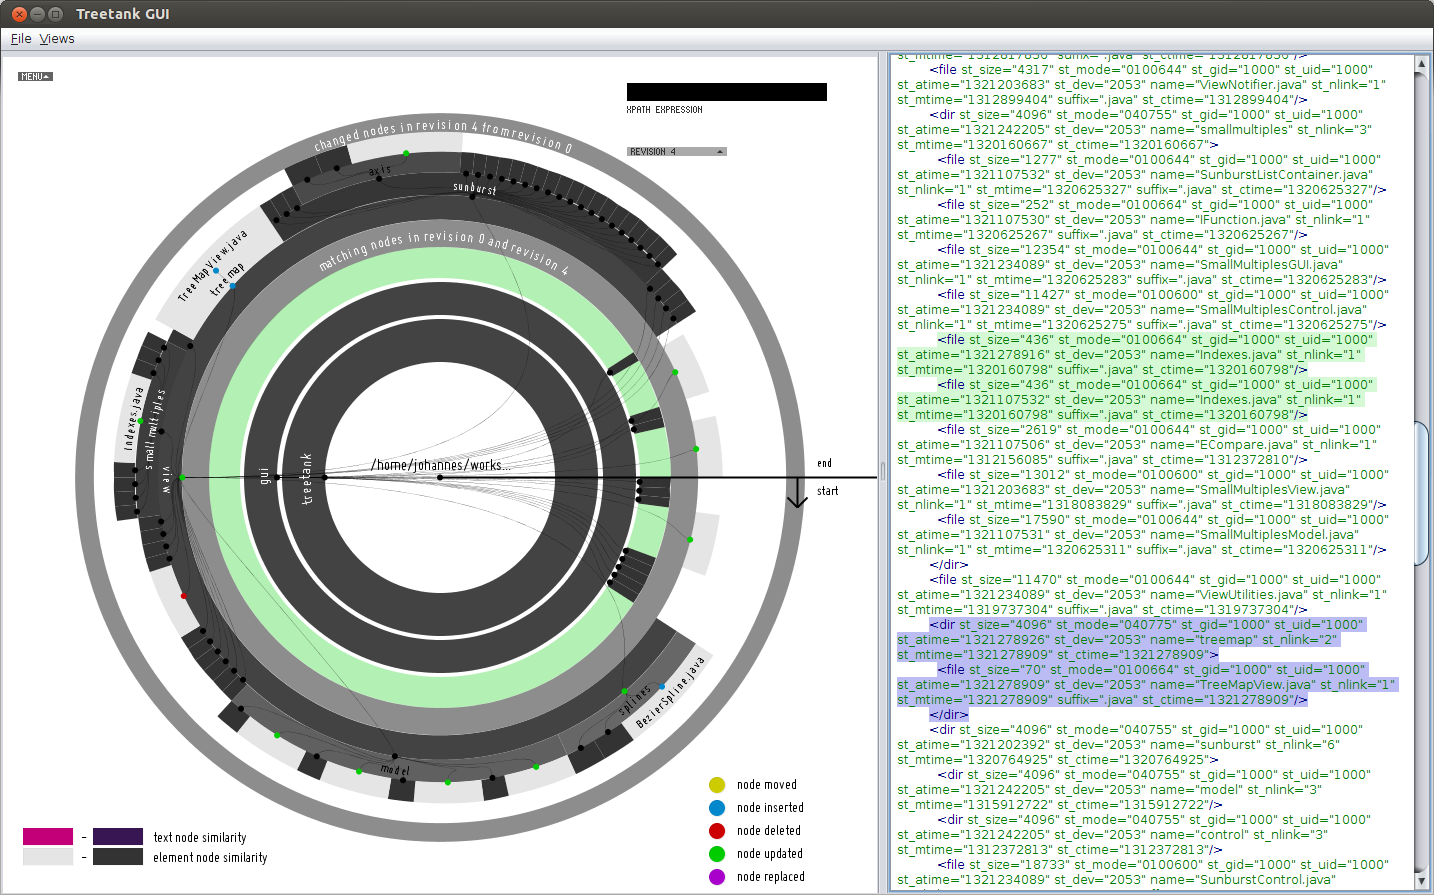
\includegraphics[width=\textwidth]
{figures/gui-fsml-fulldiff}}
\caption{\label{fig:fsml-gui-fulldiff} FSML comparsion of the GUI src-folder using a full diff including namespaces and attributes.}
\end{figure}

We conclude, that the preprocessing step of matching nodes in the FMSE-algorithm works reasonably well on FSML-data as no similar \texttt{TextNode}s are included. However we aim to support the extraction of metadata for several kinds of files which might introduce the possibility of mismatches in the future.

In order to avoid any mismatches and therefore executing too many update-operations on nodes which have not changed at all as well as to avoid the costly execution of the FMSE-algorithm in the first place the capabilities of current filesystems to register for modification-events are additionally used. The steps are as follows:

\begin{enumerate}
\item To obtain the hierarchical structure of filesystems the Java7 Filesystem-Walker API is used instead of the Python-Script. A new database is created in Treetank with a standard resource named "fsml" whereas the hierarchical structure is mapped to the resource while traversing a directory. 
\item The new \texttt{WatchService} is used to detect subsequent changes in a watched directory. In order to support watching all subdirectories as well a suitable datastructure as for instance an associative array has to be used in the first place. Java does not permit recursive watching of all subdirectories, as it is not supported by some filesystems.
\end{enumerate}

The \texttt{WatchService} detects the following events:

\begin{itemize}
\item \texttt{ENTRY\_CREATE}: File or directory has been created.
\item \texttt{ENTRY\_DELETE}: File or directory has been deleted.
\item \texttt{ENTRY\_MODIFY}: File has been modified.
\end{itemize}

Therefore moves and renames are not supported out of the box. The path to the directories and files is translated to an XPath query, which locates the appropriate node in the database/resource. In case a new file or directory has been created a new \texttt{ElementNode} is pre\-pen\-ded as a first child of the parent node as filesystem-trees are unordered. In this case the XPath-query translates the parent-path into the appropriate XPath-query, that is it is of the form \\\texttt{/dir[@name='pathComp1Name']/dir|file[@name='pathComp2Name']}. The path component usually denotes a directory whereas the last component might be a directory or file in case of an \texttt{ENTRY\_DELETE} event. Deleted directories have to be removed from a WatchService/Path-mapping in an associative array. Furthermore all paths have to be saved in another datastructure to denote if the deleted path pointed to either a file or directory. Thus another associative array is used to save a Path $\Leftrightarrow$ EPath mapping for inserted nodes. EPath is a Java enum to determine the type (file or directory). 

The FSML-subdialect currently used is very simple. Listing \ref{lst:fsml} provides an example of the simple structure. Directories are mapped to \texttt{dir}-elements, whereas files are mapped to \texttt{file}-elements. Note that the names can not be used without preprocessing to denote the elements, as for instance whitespaces are not permitted in QNames. Thus, either whitespace characters and other not allowed characters are escaped or as in our case saved as attribute-values in \texttt{name=""}-attributes. The labels in the visualizations are optionally based on this special attribute.

While this representation currently does not incorporate most of the strengths FSML usually provides it is easy to add metadata about files and to incorporate text-files. Optionally instances of custom classes are pluggable to provide any type of extensibility. Thus it is possible to provide extractors for certain types of files and to incorporate text-files into the FSML-representation itself, possibly by adding a link to another resource in the fsml-database.

\begin{code}[caption=FSML structure]
<fsml>
  <dir name="Desktop">
    <dir name="Lichtenberger">
      <dir name="Bachelor">
        ...
      </dir>
      <dir name="Master">
        <dir name="Thesis">
          <dir name="figures">
            <file name="fsml-incremental.png" suffix=".png"/>
            ...
          </dir>
          <file name="thesis.tex" suffix=".text"/>
          ...
        </dir>
        ...
      </dir>
    </dir>
    ...
  </dir>
</fsml>
\end{code}
\label{lst:fsml}

Fig. \ref{fig:fsml-itemsize-pruning} is an example of mapping the author's Desktop-folder to a database in Treetank (move- and replace-detection is disabled). Subsequent revisions are commited every five minutes.

\begin{figure}[tb]
\center{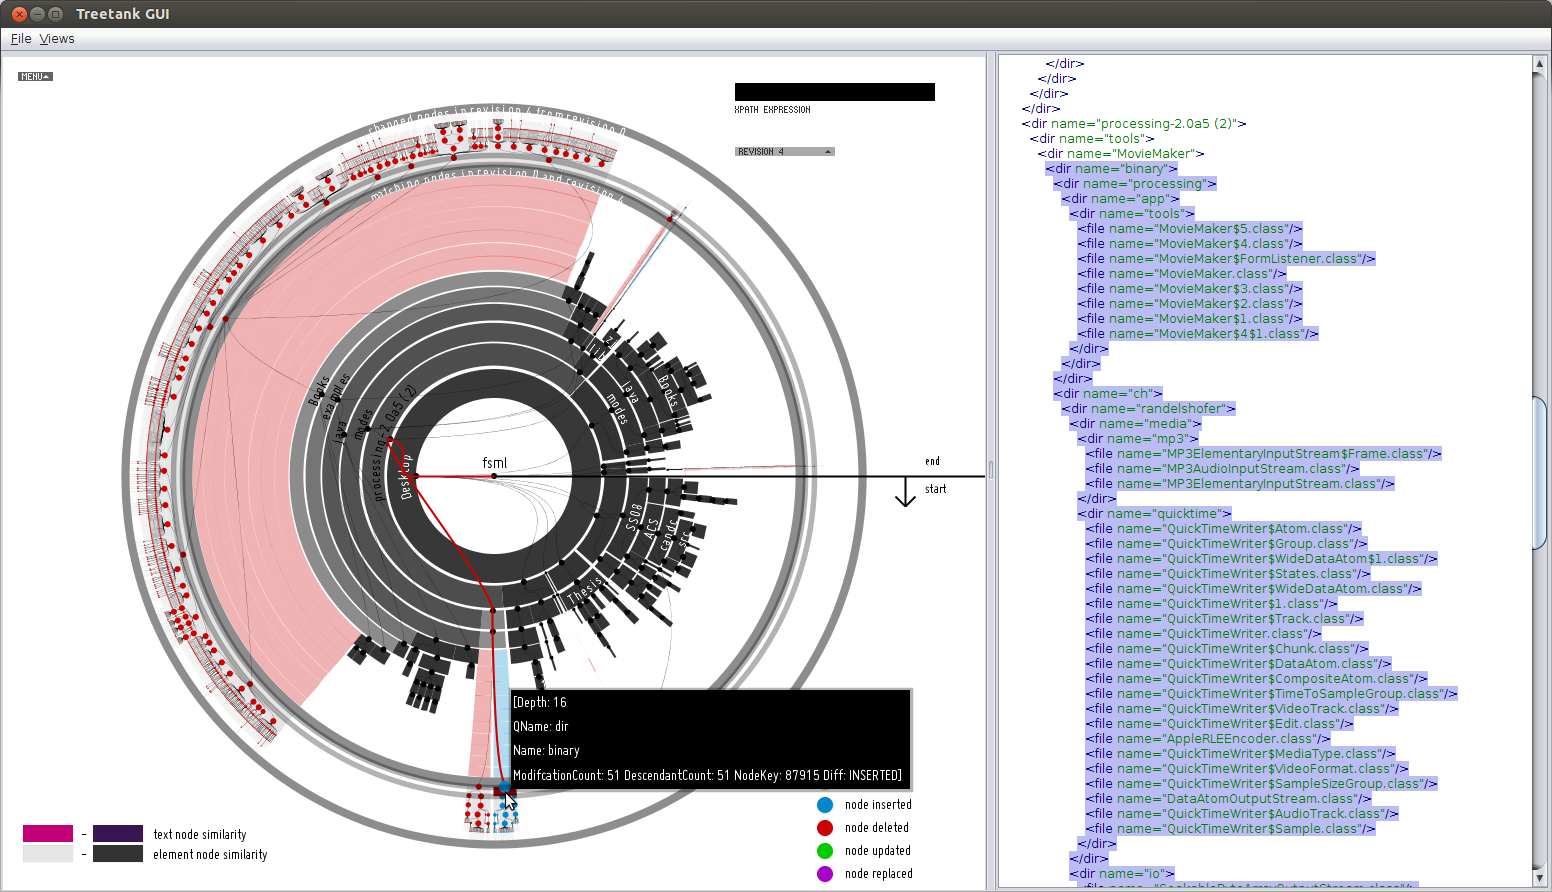
\includegraphics[width=\textwidth]
{figures/fsml-changes-itemsize-pruning.png}}
\caption{\label{fig:fsml-itemsize-pruning} FSML comparsion of the author's desktop.}
\end{figure}

Most files and directories are unchanged. Usually subtrees of changed items (besides the processing-subfolder which has been deleted) are rather small compared to most unchanged nodes. Thus, we study the effect of changing the filtering method. Pruning by same hashes instead of the itemsize is displayed in Fig. \ref{fig:fsml-pruned-by-samehashes}. Sunburst items for the large subtrees of the unchanged nodes are not generated. As a direct consequence items of interest are enlarged and thus much better visible. %Two subdirectories matching the simple XPath-query \texttt{//dir[@name='wiki-sorted']} are highlighted. It is immediately obvious that a subtree rooted at the directory named "wiki-sorted" has been deleted and another one has been inserted. The equal subtree-size suggests that the subtree has been moved. On close inspection, for instance using the subtrees rooted at "wiki-sorted" we see that the subtrees are isomorph (Fig. \ref{fig:desktop-screenshot-compare}). This might be due to the directory traversal which seems to be non-deterministic. We can suggest that the directory therefore has been moved. However in future work we aim to detect moves in the first place and therefore also use the appropriate visualization through splines explained in chapter 3. To compare the two subtrees we used two Treetank-GUI instances on the same database/resource. This is possible due to Treetank permitting multiple read-transactions.  

\begin{figure}
\centering
\subfigure[FSML comparsion of the author's desktop filtered by identical hash-values.]{
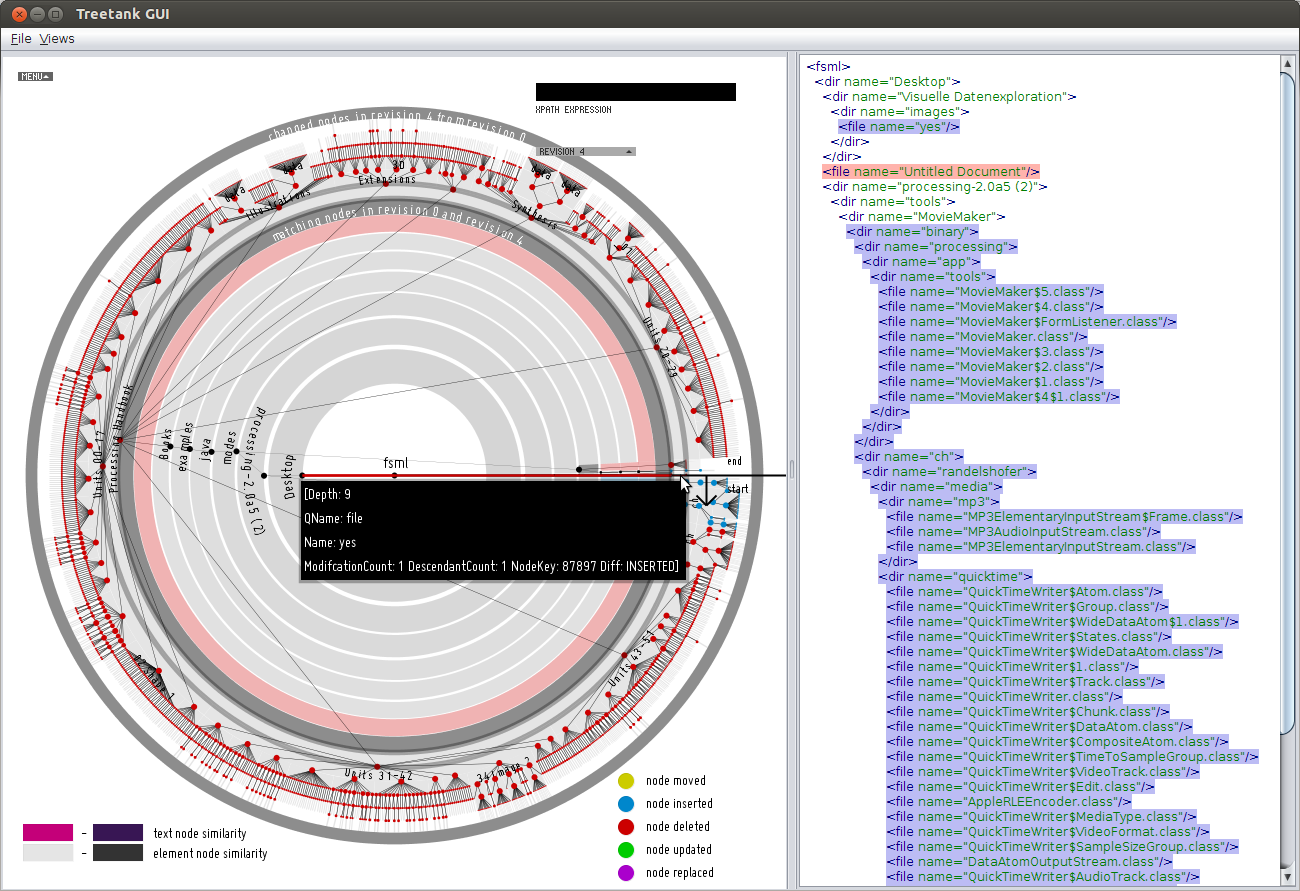
\includegraphics[width=\textwidth - 5em]
{figures/fsml-pruned-by-hashes}
\label{fig:fsml-pruned-by-samehashes}
}
\subfigure[FSML comparsion of the author's desktop (small multiple displays -- incremental view).]{
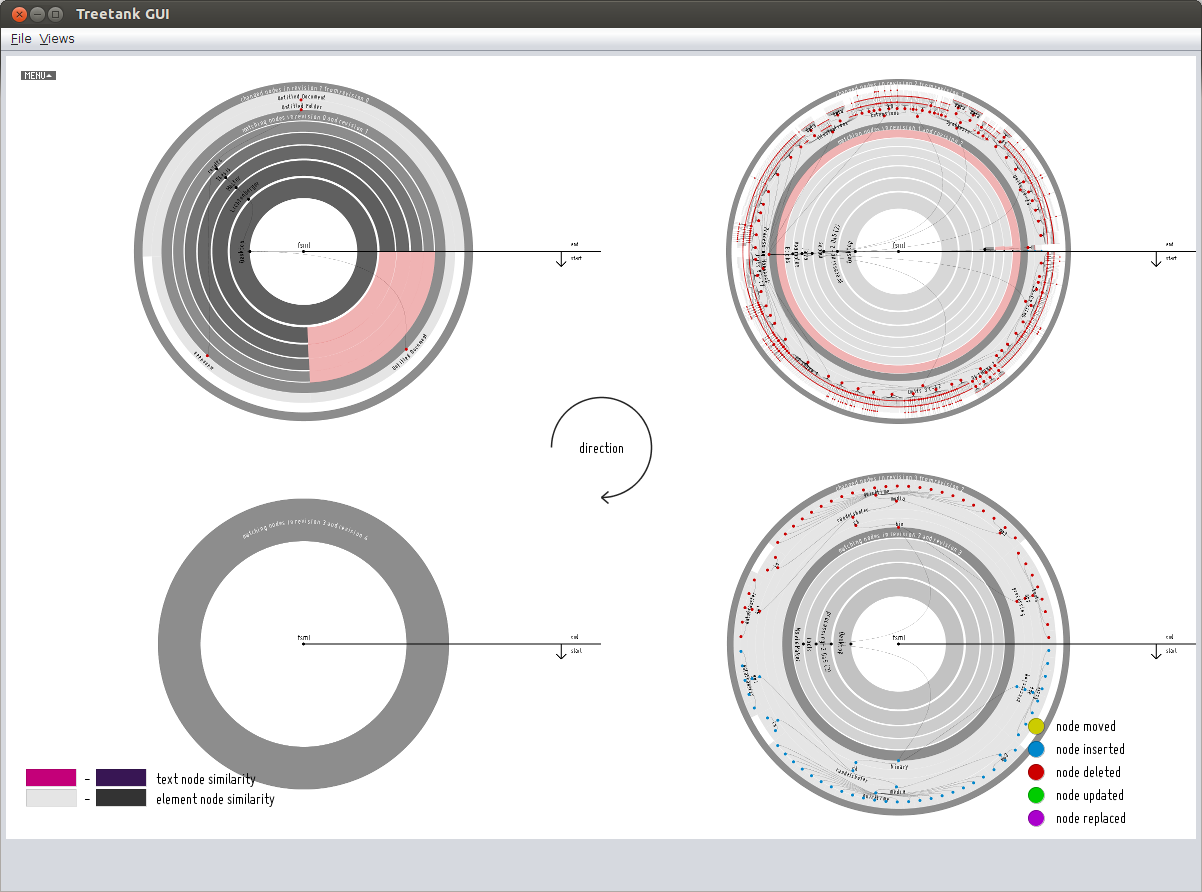
\includegraphics[width=\textwidth - 5em]
{figures/fsml-incremental-pruned-by-samehashes.png}
\label{fig:fsml-smallmultiples-incremental}
}
\caption{FSML comparison.}
\end{figure}


%\begin{figure}[tb]
%\center{\includegraphics[width=\textwidth - 7em]
%{figures/fsml-pruned-by-hashes}}
%\caption{\label{fig:fsml-pruned-by-samehashes} FSML comparsion of the author's desktop filtered by identical hash-values.}
%\end{figure}

%\begin{figure}[tb]
%\center{\includegraphics[width=\textwidth]
%{figures/desktop-screenshot-compare.png}}
%\caption{\label{fig:desktop-screenshot-compare} FSML comparsion of wiki-sorted subtrees}
%\end{figure}

%To reduce the number of \emph{SunburstItem}s and the runtime of creating the items and the offscreen buffer the tree can be pruned by itemsize, just like in the case of the wikipedia-import. Items which are too thin and thus do not add any value to the visualization are pruned. The default modification-weight is used, which is not enough to adjust and enhance the sizes of changed subtrees. Furthermore this type of pruning doesn't impose any positive effect on the subtree-size of changes. Therefore we use the pruning by hash-values (Fig. \ref{fig:desktop-screenshot-pruned-hash}), which skips any unchanged subtrees. The number of created items is reduced drastically without causing any negativ effect. The context is still visible. Furthermore the items are big enough to be readable on the highest level without zooming into subtrees by selecting a new subtree-root node.

%\begin{figure}[htb]
%\center{\includegraphics[width=\textwidth]
%{figures/desktop-screenshot-pruned-hash.png}}
%\caption{\label{fig:desktop-screenshot-pruned-hash} FSML comparsion of "/home/johannes/Desktop" pruned by same hashes}
%\end{figure}

A sequence of comparisons between several revisions is viewable with the incremental small multiple display variant (Fig. \ref{fig:fsml-smallmultiples-incremental}). We used the hash-based pruning without generating items for nodes with identical hash-values, to keep the number of items to a minimum. By hovering the items and comparing the values as well as subtree sizes we are able to determine a directory-rename between revision 2 and 3 in the bottom right view. A \texttt{rename}-operation however is not supported by the Java \texttt{WatchService} such that usually, depending on the filesystem a delete- and an insert-event in either order is received.

In general we are able to answer questions such as 

\begin{itemize}
\item Auditing: Which files are updated/inserted/deleted or not during a sequence of snapshots?
\item Does an employee adhere to company instructions regarding installed software? (by file-extensions or analysing the binaries and storing an additional attribute with "true" or "false" values)
\end{itemize}

%\begin{figure}[tb]
%\center{\includegraphics[width=\textwidth - 7em]
%{figures/fsml-incremental-pruned-by-samehashes.png}}
%\caption{\label{fig:fsml-smallmultiples-incremental} FSML comparsion of the author's desktop (small multiple displays -- incremental view).}
%\end{figure}

\subsection{Summary}
This chapter introduced a few use cases for comparing tree-structures. Depending on the activated views different characteristics are revealed. 

The smallmultiple differential-variant should be used to compare similar, different tree structures. Choosing the incremental variant reveals changes in temporal evolving trees. In case the tree is rather small (for instance less than 5000 nodes) it is arguable that the views can be used without filtering. However, once more items have to be created it is necessary to choose one of the filtering techniques to keep the numer of items small and to prune nodes/subtrees of no interest. Hovering through linking and brushing facilitates keeping track of changed nodes. When one of the pruning techniques is enabled, inserted nodes might not be visible in upcoming comparisons. However, this indicates that the items have not been changed within later revisions. 

The standard \emph{SunburstView} reveals all kinds of differences and furthermore allows two zooming operations. The zooming/panning which transforms the viewing-coordinates through affine transformations may be used if the number of items is small and therefore animations are possible whereas a left-mouseclick on an item transforms the item into a new root-node. As already explained in Chapter \ref{sec::visualizations} this involves either a transformation based on node-copies and adjusting angles or the full pipline has to be passed in case of the itemsize-pruning.

We have merely scratched the surface of the possibilities of our current approach. The small multiple displays will greatly benefit from a temporal XPath-extension. Some proposed axis as \texttt{next::}, \texttt{previous::}, \texttt{future::}, \texttt{past::}, \texttt{revision::} already have been implemented but have to be incorporated in an XPath/XQuery-engine. Simple queries as for instance \\\texttt{//dir[@name='wiki-sorted']/future::node()} will reveal nodes with the attribute \\\texttt{name='wiki-sorted'} in all future revisions. The start-context will be based on the currently opened base-revision. 

\cleardoublepage
\section{Discussion}\label{sec::discussion}
\subsection{Introduction}
This Chapter concludes the main contribution of this thesis with a discussion of the work presented in relation to the state-of-the-art.

The presented approach facilitates the comparison of tree-structures through various linked visualizations showing the tree-structures at varuous levels of detail. The Small multiple variants of a \emph{SunburstView} provide a high level view of the differences between many tree-structures. Linking and brushing is used to highlight nodes in all small visualizations. The \emph{SunburstView} itself incorporates both a mode to visualize one tree-structure and a mode to visualize comparisons between two tree-structures. A new layout-algorithm has been developed to highlight changes in a prominent place. Furthermore different filtering methods allow the comparison of large trees. Details are shown on demand through a mouseover effect and a linked \texttt{TextView}. A selection of a new root-node togehter with a simple undo-operation allows to drill down into the tree as known from other Sunburst-visualizations. However costly recalculation of diff-tuples, modifications and descendants of each node is omitted in all cases but the itemsize-based pruning. Instead we recalculate the maximum depth of unchanged nodes and scale a new list of items to fit the new boundaries. The \texttt{TextView} provides a low-level serialization of (sub)trees linked with the \texttt{SunburstView} also tailored to large tree-structures.

Unlike other visualizations of tree comparisons we have found and described in Chapter \ref{sec::relwork} our approach is entirely database driven. The DBMS is tailored to temporal tree-structures which are stored as snapshots. Each node in the database/resource is unique and remains stable throughout all revisions. As most trees do not inhibit node-IDs we have implemented an ID-less diff-algorithm called FMSE to import differences. Afterwards we are able to use a faster diff-algorithm based on the node-IDs and furthermore are able to utilize hashes to further speed up the algorithm. Due to FMSE our similarity-measure between trees is based on a matching algorithm which computes the longest common subsequence (LCS) bottom up and furthermore tries to find cross-matches of unmatched nodes.

Most proposed visualizations in contrast rely on stable unique IDs (the Contrast Treemap\cite{tu2007visualizing}, Code Flows\cite{telea2008code}, TreeJuxtaposer\cite{munzner2003treejuxtaposer} (unique node labels)) and do not include the detection of \texttt{replace}- and \texttt{move}-operations. However Code Flows visualizes moves due to spline connections between matching nodes with the same ID in two adjacent icicle plots. Due to the reliability on unique node IDs these visualizations do not cover trees which do not include unique node-IDs. In contrast our prototype is able to determine and visualize these tree-structures utilizing the FMSE-algorithm to import differences through similarity metrics for leaf- and inner-nodes.

The next section evaluates our approach similar to Chapter \ref{sec::relwork} according to several attributes.

\subsection{Evaluation Criteria}

\begin{itemize}
\item \emph{SpaceFilling} Space filling techniques try to maximize the usage of available screen space and thus facilitate a higher information density. Sunburst layouts are generally space filling, but in contrast to Treemaps lack space filling properties in the corners. However in our case the corners are used to display GUI components and legends. The small multiple variants currently have too much unused space which is due to the often times non squarified screen viewport depending on the extends of the main window. As we just scale each visualization of the comparison of each two revisions the small multiple variants currently include too much unused space due to often times non squarified screen viewport which depends (1) on the size of the main window and (2) how many visualizations are currently enabled. Thus, in a future version we will use a squarified clip of the view depending on the maximum depth to generate minimized offscreen buffers for the four regions. Other space filling approaches include Icicle plots (Code Flows) which are comparable in space consumption as always the two complete tree-structures to compare are plottet. In our case unchanged nodes are not plotted twice. Furthermore a special stable Spiral-Treemap layout has been proposed which utilizes all available screen space and remains relatively stable after changes. Usual Treemap layouts suffer from abrupt layout changes during modifications of the underlying data.
\item \emph{Hierarchy} The Hierarchy in Sunburst layouts is very well depicted due to the adjacency based layout whereas it is not as obvious in Treemaps which encapsulate child items. Cushion Treemaps have been developed for better readability of hierarchical relationships using shading. However they are still not as good readable as in adjacency based layouts. Code flows utilizes Icicle plots which are rectangular views of the radial Sunburst layout, thus adjacency based and very well readable. Our approach optionally plots a node-link diagram on top of the Sunburst layout to further illustrate the relationships such that the hierarchy is at least as well depicted as in other node-link diagrams (for instance in TreeJuxtaposer and Treevolution). 
\item \emph{Readability} To both use node-link diagrams and a Sunburst layout facilitates a higher information density as individual nodes can be color-coded as well as their child/parent relationship, the links between the nodes. Thus we are able to utilize to map certain attributes to the extension of the Sunburst items, the color of the arcs, the color of the dots/nodes in the node-link diagram. To maximize the information density we could also use histograms in the Sunburst items instead of just using one color for the whole item. However we assume that usually the items will be too small, such that a whole histogram would possibly not be readable in many cases. To support better readability of item-labels our visualization is able to be rotated. Node labels of Treemaps and Icicle plots however usually are better readable due to their rectangular display in comparison to circular plotted labels. Thus the \emph{TextView} has been extended to take the agglomerated tree-structure into account. It is an ideal partner of the \emph{SunburstView} as it provides better readability of small subtrees but lacks the overall overview about all differences provided by the \emph{SunburstView}. 
\item \emph{Similarity of ID-less tree-structures} Some proposed tree-to-tree comparsion visualizations depend on node-IDs (Spiral-/Contrast-Treemap\cite{tu2007visualizing}) or the comparison technique has not been meantioned. Others depend on domain characteristics (Treejuxtaposer\cite{munzner2003treejuxtaposer}, Code Flows\cite{telea2008code}). Juxtaposer seems to rely on unique leaf node labels. Otherwise it is not obvious how to map node labels to their postorder rank on a region plane. In contrast to Treejuxtaposer and other proposed systems our prototype is able to compare every kind of tree-structure.
\item \emph{Structural changes} Our visualizations, in particular the \emph{SunburstView} and the small multiple display variants support the highlighting of all kind of structural-changes (inserts, deletes, updates, replace and move-operations) through color-coded nodes. In case of moves- links, currently depicted as arrows, denote the movement from their original- to their target-place using hierarchical edge bundling to avoid or at least reduce visual clutter due to overlapping lines or curves. Furthermore the extend of the sunburst items is based on the nodes' subtree size \emph{and} the number of modifications in the subtree. Most other visualizations do provide a global distortion to further emphasize changes except Treejuxtaposer to the best of our knowledge.
\item \emph{Non structural changes} in \texttt{TextNode}s are color coded to denote that the value is \texttt{UPDATED} through coloring the node in the overlapping node-link diagram accordingly. Furthermore the color of the SunburstItem reflects their similarity using a Levenshtein String comparison.
\item \emph{Filtering} is one of our primariy concerns. The focus of this thesis evolved around comparing Treetank-resources. As Treetank is a secure storage system it naturally often times stores very large tree-structures. Thus our first consideration was to filter items which can be perceived, that is too small items are not created. However this only effects the creation of SunburstItems and does not concern the ID-based diff-algorithm. To speed up both, the ID-based diff algorithm as well as the construction of SunburstItems we developed the diff-algorithm which skips subtrees with same hashes and moves both transactions to the next node on the XPath-following axis. Thus, in case large subtrees can be skipped the diff-algorithm using hash-comparisons is much faster. Besides even less items have to be created and in case of a subtree-selection only the itemsizes have to be recalculated instead of reinvoking the diff-algorithm, recalculate the descendant- and modification-count, and the whole preorder traversal of the agglomerated tree-structure with all stack-adjustements. Pushing the idea of filtering by hashvalues to its limits involves to avoid the creation of SunburstItems for the nodes, which have the same hashvalues. These filtering techniques furthermore enlarge changed subtrees naturally as the arc of the items is based on the \emph{subtree-size} of each node and the number of \emph{modifications} therein. TreeJuxtaposer once more along with Code Flows to the best of our knowledge seem to be the only systems which are able to handle large tree-structures but the diff-algorithm of TreeJuxtaposer relies on unique node labels. Code Flows does not provide a global filtering method such that their filtering is comparable with our method to drill down into the tree. However, due to filtering by queries the filtering is mightier. Implementing such a behavior in our prototype will be straight forward allowing the user to specify an XPath-query and invoke the diff-algorithm for each result on both revisions. Our current approach is able to filter differences and related context nodes on a global basis and on subtrees once a user drilled down into the Sunburst visualization with a guaranteed visibility of modifications much like in TreeJuxtaposer.
\end{itemize}

\todo{Nochmal Tabelle mit Vergleich zu allen anderen im related work kapitel beschriebenen visualisierungen}

\cleardoublepage
\section{Summary, Conclusion and Future Research}\label{sec::conclusion}
\subsection{Summary}
A full pipeline has been implemented backed by the secure tree-storage system Treetank ranging from (extensive) preprocessing to ID-less and ID-based diff-algorithms to new layout algorithms developed for 

Almost all data is subject to preprocessing. In the case of Wikipedia we aimed at comparing the temporal evolution of several articles. The Wikimedia Foundation provides only full Wikipedia dumps which aren't sorted by revision-timestamps. Therefore it had to be sorted at first using Hadoop. Importing structural changes which should be revealed by the visualizations afterwards requires a diff-algorithm which doesn't operate on unique node IDs. Thus the FMSE-algorithm described in Chapter \ref{sec::relwork} and \ref{sec::differences} has been implemented as well as several missing edit-operations in Treetank (\texttt{copy}, \texttt{move}, \texttt{replace}), whereas others have been extended to adhere to the XPath/XQuery Data Model (XDM) to simplify the internal ID-based diff-algorithm and to add to the visualizations' expressiveness (no two adjacent text-nodes are ever created). The FMSE-algorithm is furthermore useful to compare generic trees. In this case structural changes between a base tree and several other trees are imported consecutively which are visualized by the SmallMultiples differential view in a subsequent step. Other studied applications include the comparison of snapshots of a directory in a filesystem and two revisions of XML-exported LFG-grammars.

An ID-based diff-algorithm has been developed to compare imported data based on snapshots/revisions, whereas the comparison is \emph{not} restricted to both subsequent revisions and whole documents. A fast version utilizes hash-values of each node generated during the import. These are derived from the nodes' descendants and used to reduce the run-time of the algorithm. The algorithm can skip the comparison of the whole subtree of every node with a matching hash-value.

The visualizations trigger the ID-based diff-algorithm if needed. A \emph{SunburstView} based on aggregated tree-structures is one of the major contributions. Drawing a new Sunburst-layout for a selected-node to drill down into the tree doesn't require the invocation of the diff-algorithm. A notable exception is the itemsize-based pruning because the diffs are usually not saved to avoid their constant in-memory space consumption. Instead they are usually subject to garbage collection. The type of diff however is saved as part of the created Sunburst item and used by the visualization. 

A new Sunburst layout algorithm has been designed to specifically support the analysis of structural changes, which are featured prominently between two rings whereas the first inner ring denotes the maximum depth of unchanged nodes and the second denotes the maximum depth of changed nodes. The first changed node in a subtree is semantically zoomed from its original place (the depth is increased) to reside between the two rings supporting a tree-ring metapher based on the analogy of an aging tree in the nature which adds growth rings every year.

The variant of the \emph{SunburstView} which has been designed to compare tree-structures furthermore incorporates three filtering methods. First, an itemsize based approach to filter nodes based on their extend is provided. It is used to speed up the creation of the Sunburst items, but does not effect the run-time of the diff-algorithm used in the first place. Second, a method utilizing the hash-based diff-variant skips whole subtrees of unchanged nodes and thus builds solely interesting items to the task at hand (which is analysing structural changes). A third variant even skips the creation of building items for nodes with unchanged content altogether. This variant is especially interesting for very large tree-structures to keep the memory consumption to a minimum and to provide maximum space for subtrees which contain changed nodes.

Besides filtering uninteresting nodes automatically reducing the run-time of the diff-algorithm and/or the creation of Sunburst items and reducing in-memory space consumption sometimes it is interesting to view the whole aggregated tree in an overview. To still emphasize structural changes the extend of an item is based on the \texttt{descendant-or-self} count of a node as well as of its modification count, whereas the amount which one affects the extend at most can be chosen by a slider. Note that the modification-count is based on the number of modification in the nodes' subtree as well as on a constant factor the which is multiplied as modifications are usually small compared to the whole tree plus the addition of the \texttt{descendant-or-self} count as a fallback which needed in case of zero modifications in the subtree. The addition is needed in case of the slider to adjust how much the modifications contribute to the extension is set to zero, such that the extend is solely based on the \texttt{descendant-or-self} count.

In addition to the enhanced \texttt{SunburstView} supporting comparisons several \emph{SmallMultipleView} variants, based on the \emph{SunburstView} have been developed to support an overview about the changes ranging up to the comparsion of currently at most five revisions. An incremental version displays changes related to a sliding window of two subsequent revisions. The left upper view shows a comparison between the loaded baseRevision and $baseRevision + 1$, the right upper view displays the comparision between $baseRevision + 1$ and $baseRevision + 2$ whereas the comparsion between two subsequent revisions is done clockwise until either no more revisions are available or five revisions have been compared (all four squarified regions are filled with Sunburst views). A differential version compares subsequent revisions to the loaded baseRevision. This version is ideal to compare different tree-structures to a reference tree. A hybrid view first compares the baseRevision with the last revision which can be drawn in the bottom left square of the visualization. Subsequently it computes differences just like in the incremental version but blackens changes which occur in subsequent incremental comparisons.

\subsection{Conclusion}
In retrospective the goals described in the introduction have been achieved. The GUI-frontend embedding the visualizations aids analysts in comparing tree-structures ranging from temporal to generic similar trees. Its main strength is the comparison of structural changes, whereas a smilarity-measure for \texttt{element}-nodes depends on the amount of overlapping nodes in its subtree. In contrast \texttt{text}-nodes are compared based on the Levenshtein-algorithm as \texttt{text}-nodes are always leaf-nodes in a tree. Other algorithms might be easily included for instance to compare numerical values.

Our approach based on a tight storage integration integrates several edit-operations utilizing an expressive aggregated tree-structure build through observing diffs from the ID-based diff algorithm. The ID-based algorithm supports two modes. Either only structural nodes (\texttt{DocumentNode}, \texttt{ElementNode} and \texttt{TextNode}s) are compared or structural and non structural nodes (adding \texttt{NamespaceNode}s and \texttt{AttributeNode}s). The encountered diffs are saved in an associative array and further processed to construct a novel Sunburst layout tailored to tree-comparisons. In contrast to other visual tree-comparison tools our prototype incorporates several edit-operations including moved and replaced nodes which are rarely seen in other visualizations. Filtering-mechanisms facilitate the comparison of very large tree-structures. Note that no other approach described in Chapter \ref{sec::relwork} to the best of our knowledge incorporates such filters and therefore most likely is not useful to inspect large datasets. Two filtering mechanisms depend on hashes which are used to compare the whole subtree of a node including itself. Subtrees are skipped from comparison if the hashes are identical. Thus they are neither traversed nor items are build subsequently. Besides building an aggregated tree-structure from observing changes by the ID-based diff-algorithm no state is involved. Unlike the straight forward approach of building two in memory datastructures with nodes of both revisions which are going to be compared our algorithm uses less space and is much faster. Furthermore a new Guava based cache preloads node pages in a dedicated thread and thus facilitates faster traversal of large tree-structures.

In addition to a novel Sunburst layout we implemented three different \emph{SmallMultiplesView} variants. Two of them, the incremental- and the differential-view compute the diffs and the subsequent visualizations in each of the four screen regions (top-left, top-right, bottom-right, bottom-left assuming five subsequent revisions of the tree-structure to compare exist) in parallel. On mouse-over items are highlighted in each region in which they are present. Compared to an icicle-view which connects unchanged items in each revision by splines our approach features changes much more prominently through the semantic zoom/the tree-ring metapher as well as a modifyable modification-rate. A hybrid variant currently suffers from the lack of visual 

\subsection{Future Research}
Many topics are subject to further research. 

\begin{itemize}
\item First of all we want to incorporate the temporal XPath axis in an XQuery processor, most probably Brackit\cite{Brackit}, which is especially important to further analyse tree-structures. Therefore it will be inevitable to provide indexes for fast response-times of the visualizations.
\item The plotting of moved nodes will be based on Hierarchical Edge Bundles with a line gradient color, whereas most work has already been done.
\item Building an index structures for visualizations of consecutive revisions (the SmallMultiples incremental-view).
\item Writing a proper StAX-implementation to iterate directly through the diffs to better support the \texttt{TextView}.
\item Evaluation and integration/implementation of various other tree-similarity measures.
\end{itemize} 


%%%%%%%%%%%%%%%%%%%%%%%%%%%%%%%%%%%%%%%%%%%%%%%%%%%%%%%%%%%%%%%%%%%%%%%%%%%%%%%%%%%%%%%%%%%%%%%%%%%%%%%%%%%%%%%%%
%%% APPENDIX
%%%%%%%%%%%%%%%%%%%%%%%%%%%%%%%%%%%%%%%%%%%%%%%%%%%%%%%%%%%%%%%%%%%%%%%%%%%%%%%%%%%%%%%%%%%%%%%%%%%%%%%%%%%%%%%%%
\cleardoublepage
\appendix
\section{Treetank}\label{sec::treetank}

\subsection{General persistent storage enhancements}\label{subsec::storage}
While not exclusively developed for our tree-to-tree comparsion for completeness we want to meantion several techniques which have recently been developed to support the persistent storage of large tree-structures efficiently (with a minimum space overhead).

\begin{itemize}
\item Values of \texttt{TextNodes} are compressed by using the Deflate-algorithm which combines the LZ77 algorithm and Huffman coding. Decompressed values are cached in memory once they are requested. Furthermore only values which are greater than a certain length-threshold are compressed.
\item Pointers to neighbour nodes, the first child and the parent node are persisted as ranges.
\item As ranges are persisted node-IDs are efficiently compressed.
\item Whole \texttt{NodePage}s are compressed using the very fast Snappy-algorithms due to a lot of compression/ decompression in case of many modifications of the same NodePage in the BerkeleyDB log.
\item In case of the \texttt{DocumentNode} only the firstChild-pointer and descendant-count has to be persisted. Similar the serialization of \texttt{TextNode}s doesn't include the childCount and descendantCount as well as the firstChild-pointer.
\item The \texttt{NamePage} which is used to store String-names which are commonly repeated in XML-documents now contains index-mappings whereas we opted for different indexes based on an element-QName index, an attribute-QName index and a namespace/URI-index. This allows an XPath- or XQuery- Optimizer to use the index for queries as \texttt{count(//@attribute='foo')} or\\ \texttt{count(//element()='bar')}. We furthermore aim to provide backreferences to the nodes as we encountered far too long response-times on larger tree-structures. A path-like index therefore might be inevitable in the long term.
\item Deletion of \texttt{attribute}- and \texttt{namespace}-nodes in subtrees.
\end{itemize}

\subsection{ACID properties}\label{subsec::acid}
Consistency rules have been enhanced while developing our prototype. The following provides a brief overview about the ACID-properties of Treetank.

\begin{enumerate}
\item \emph{Atomicity} is ensured through the transaction layer and the interchangeable backend (currently BerkeleyDB). As such atomicity is even guaranteed in case of power failures, errors and crashes.
\item \emph{Consistency} as of now involves the checking of \texttt{QName}s for validity. At all times no adjacent text nodes are created which is consistent with the XPath/XQuery Data Model (XDM). We also introduced XML entity encoding for the XML characters serialization (in the \texttt{XMLSerializer} as well as the new \texttt{StAXSerializer} and \texttt{SAXSerializer}). Furthermore we check attribute \texttt{QName}s for duplicates and throw an appropriate runtime exception if a new attribute insertion would yield duplicates. Similarly insertion of duplicate namespace prefixes for namespaces of the same parent element-node are prohibited.
\item \emph{Isolation} is guaranteed through \emph{Snapshot-Isolation} which is based on the transaction-, page- and I/O-layer through versioning. Furthermore currently only one write transaction is allowed per resource. To maximize the properties of tree-structures the implementation of concurrent write-transactions on different subtrees with appropriate locking is in development.
\item \emph{Durability} is guaranteed through the backend. The transaction log created by Treetank's BerkeleyDB-binding implemented as a cache to store all changed pages and nodes is written and flushed on transaction commit.
\end{enumerate}

\subsection{Axis}
The axis in Treetank have been changed to adhere to the \texttt{hasNext()} and \texttt{next()} specifications of the \texttt{Iterable} interface. The check if \texttt{getNext()} is true is added to all axis such that \texttt{hasNext()} is idempotent. It simply checks a flag which is set in \texttt{resetToLastKey()} to make sure the transaction points to the node after the last call to \texttt{hasNext()} without changing the node-ID to which to move in the next call to \texttt{next()}. Furthermore the transaction now is not moved forward in \texttt{hasNext()} anymore which is done only when calling \texttt{next()}. Instead a variable denoting the next node-ID is set which is used by the \texttt{next()} implementation to move to the next node. Furthermore \texttt{next()} now also is idempotent, simply checking if it has been called before. When true and \texttt{hasNext()} has not been called immediately before it is first called by \texttt{next()}.

\subsubsection{Levelorder-Axis}\label{subsubsec::levelorderaxis}
The \texttt{LevelOrderAxis} is described in algorithm \ref{levelOrderAxis}. Just like other axis to traverse certain regions or the whole tree-structure in Treetank it is based on the \texttt{Iterator/Iterable} Java interfaces to support the \texttt{foreach}-loop and iterator-based iteration. All other axis are changed as described in Appendix \ref{sec::treetank}. \emph{mFirstChilds} is a double ended queue to remember all first childs of each node for a subsequent new depth ($depth + 1$). \texttt{processElement()} is invoked to add non structural nodes, that is \texttt{attributes} and \texttt{namespaces} to the queue. After initialization the queue is empty and \emph{mNextKey} is initialized to either the current key (if self is included), the right sibling node key if there is one or the first child node key. The NULL\_NODE\_KEY is a special node key to denote that the traversal is done.

\begin{algorithm}[Hhtbp]
%\SetAlgoLined
\SetKwInOut{Input}{input}\SetKwInOut{Output}{output}
\Input{boolean mFirst, Deque mFirstChilds, long mKey}
\Output{node key of next node}
\BlankLine
\If{getNext()}{
  return true\;
}
  
resetToLastKey()\;

\tcp{Setup.}
INodeReadTrx rtx $\leftarrow$ getTransaction()\;
IStructNode node $\leftarrow$ rtx.getStructuralNode()\;

\tcp{Determines if it is the first call to hasNext().}
\If{mFirst == true}{
  mFirst $\leftarrow$ false\;
  return processFirstCall()\;
}

\tcp{Follow right sibling if there is one.}
\If{node.hasRightSibling()}{
  processElement()\;
  \tcp{Add first child to queue.}
  \If{node.hasFirstChild()}{
    mFirstChilds.add(node.getFirstChildKey())\;
  }
  mKey $\leftarrow$ node.getRightSiblingKey()\;
  return true\;
}

\tcp{Iterate over non structural nodes (attributes/namespaces).} 
\If{mInclude == EInclude.NONSTRUCTURAL}{
  processElement()\;
}
\tcp{Add first child to queue.}
\If{node.hasFirstChild()}{
  mFirstChilds.add(node.getFirstChildKey())\;
}

\tcp{Then follow first child on stack.}
\If{!mFirstChilds.isEmpty()}{
  mKey $\leftarrow$ mFirstChilds.removeFirst()\;
  return true\;
}

\tcp{Then follow first child if there is one.}
\If{node.hasFirstChild()}{
  mKey $\leftarrow$ node.getFirstChildKey()\;
  return true\;
}

\tcp{Then end.}
resetToStartKey()\;
return false\;
\caption{LevelOrderAxis (hasNext())}\label{levelOrderAxis}
\end{algorithm}

\subsection{Edit operations}\label{subsec::operations}
The \texttt{copy}-operation adds the capability to add whole subtrees of another resource or revision to the currently opened \emph{resource/revision}. Actually three \texttt{copy}-operations exist. Either the subtree is inserted as a \texttt{first\-Child}, \texttt{rightSibling} or \texttt{leftSibling} of the currently selected node. The node to copy must be a structural node, that is either an \texttt{ElementNode} or a \texttt{TextNode}. In case the transaction is located at a \texttt{DocumentRootNode} which is a special document node, which can not be deleted and exists in every revision the read transaction has to move to the first child in the first place.

%Algorithm \ref{visitTextNode} describes the handling of \texttt{TextNode}s. However, more interesting are \texttt{ElementNode}s (algorithm \ref{visitElementNode}). The algorithm recursively calls itself (\texttt{mRtx.getNode().acceptVisitor(this)}) to copy the whole subtree. To ensure that only subtrees are copied and no other nodes in document order, the depth starting at zero must be at all times $>0$ except for the root of the subtree to insert.

%\begin{algorithm}[Hhtbp]
%\SetKwInOut{Input}{input}\SetKwInOut{Output}{output}
%\Input{INodeReadTrx mRtx, EInsert mInsert, TextNode pNode, int mDepth}
%\Output{void (none)}
%\BlankLine
%mRtx.moveTo(pNode.getNodeKey())\;
%mInsert.insertNode(mWtx, mRtx)\;

%\If{!mFirst $and$ mRtx.getStructuralNode().hasRightSibling()}{
%  mRtx.moveToRightSibling()\;
%  mInsert $\leftarrow$ EInsert.ASRIGHTSIBLING\;
%  mRtx.getNode().acceptVisitor(this)\;
%}\ElseIf{!mFirst}{
%  insertNextNode();
%}
%\caption{visitNode(TextNode pNode))}\label{visitTextNode}
%\end{algorithm}

%\begin{algorithm}[Hhtbp]
%\SetKwInOut{Input}{input}\SetKwInOut{Output}{output}
%\Input{INodeReadTrx mRtx, EInsert mInsert, int mDepth, ElementNode pNode}
%\Output{void (none)}
%\BlankLine
%mRtx.moveTo(pNode.getNodeKey())\;
%mInsert.insertNode(mWtx, mRtx)\;
%mInsert $\leftarrow$ EInsert.ASNONSTRUCTURAL\;

%\For{int i $\leftarrow$ 0, nspCount $\leftarrow$ pNode.getNamespaceCount(); i $<$ nspCount; i++}{
%  mRtx.moveToNamespace(i)\;
% mInsert.insertNode(mWtx, mRtx)\;
%  mRtx.moveToParent()\;
%}

%\For{int i $\leftarrow$ 0, attrCount $\leftarrow$ pNode.getAttributeCount(); i $<$ attrCount; i++}{
%  mRtx.moveToAttribute(i)\;
%  mInsert.insertNode(mWtx, mRtx)\;
%  mRtx.moveToParent()\;
%}

%\If{pNode.hasFirstChild()}{
%  mFirst $\leftarrow$ false\;
%  mInsert $\leftarrow$ EInsert.ASFIRSTCHILD\;
%  mRtx.moveToFirstChild()\;
%  mDepth+=1\;
%  mRtx.getNode().acceptVisitor(this)\;
%}\ElseIf{!mFirst $and$ paramNode.hasRightSibling()}{
%  mInsert $\leftarrow$ EInsert.ASRIGHTSIBLING\;
%  mRtx.moveToRightSibling()\;
%  mRtx.getNode().acceptVisitor(this)\;
%}\ElseIf{!mFirst}{
%  insertNextNode()\;
%}
%\caption{visitNode(ElementNode pNode))}\label{visitElementNode}
%\end{algorithm}

%\begin{algorithm}[Hhtbp]
%\SetKwInOut{Input}{input}\SetKwInOut{Output}{output}
%\Input{INodeReadTrx mRtx, INodeWriteTrx mWtx, EInsert mInsert}
%\Output{void (none)}
%\BlankLine
%\While{!mRtx.getStructuralNode().hasRightSibling() and mDepth $>$ 0}{
%  mRtx.moveToParent()\;
%  mWtx.moveToParent()\;
%  mDepth-=1\;
%}

%\If{Depth $>$ 0}{
%  mInsert $\leftarrow$ EInsert.ASRIGHTSIBLING\;
%  \If{mRtx.getStructuralNode().hasRightSibling()}{
%    mRtx.moveToRightSibling()\;
%    \tcp{Recursion.}
%    mRtx.getNode().acceptVisitor(this)\;
%  }
%}
%\caption{insertNextNode()}\label{insertNextNode}
%\end{algorithm}

The \texttt{move-} operation just like the \texttt{copy-} operation is implemented in three different versions, \texttt{moveSubtreeToFirstChild(long)}, \\\texttt{moveSubtreeToRightSibling(long)} and \texttt{moveSubtreeToLeftSibling(long)}. Details are omitted, however the new constraint that at no time no adjacency text nodes are allowed as well as keeping the child-count of parent nodes and the descendant-count of ancestor nodes before and after a move consistent adds a lot of complexity. %The third operation is a simple wrapper for the other two, depending on the fact if a left sibling of the current node exists or not. The only parameter is the unique node ID of a node to move along with its descendants. Adjacent text-node merging adds a lot of complexity which affects the childCount and descendantCount of both the old parent node before moving a subtree and the new parent after moving. The move-operations preserve the unique node-ID and therefore are not atomic wrappers for delete- and  subsequent insert-operations or vice versa.

%We examine both operations independently as they require different node manipulations of neighbour nodes including the new and old parent node and the first child node. Both operations are defined in terms of moving structural- and non-structural nodes (the latter in subtrees of the moved node), whereas the root-node to move must be a structural node.

%First, the following constraints are checked:

%\begin{itemize}
%\item The node/subtree to move must be an \texttt{element}- or a \texttt{text}-node.
%\item It is not permitted to move a node to one of its descendants which would introduce , therefore it is checked if the node to move is one of the ancestors of the anchor node.
%\end{itemize}

%The two operation require the following node manipulations. The location the node is moved away is subject to the following changes:
%\begin{itemize}
%\item In case of \texttt{moveSubtreeToFirstChild(long)}: Parent node must point to the right sibling node key of the current node if it was the first child.
%\item Decrement child count of parent node.
%\item Collapse text nodes if both the left- and right- sibling are text nodes, therefore remove the right node and append its value to the left sibling. Furthermore adapt its right sibling pointer to the former right sibling of the right sibling text node which has been deleted.
%\item If no text node collapsing involved: adapt right sibling key of former left sibling to the right sibling key of the moved node provided one exists.
%\item If no text node collapsing involved: adapt left sibling key of former right sibling to the left sibling key of the moved node provided one exists.
%\end{itemize}

%The node to which the new subtree is inserted is subject to the following changes. \\
%In case of \texttt{moveSubtreeToFirstChild(long)}:
%\begin{itemize}
%\item Increment the child counter of the node to which the new subtree is inserted.
%\item Adapt the first child key of the node to which this node is inserted to point to the new node.
%\item Adapt the left sibling pointer of the former first child to the root node of the inserted subtree.
%\end{itemize}

%In case of \texttt{moveSubtreeToRightSibling(long)}:
%\begin{itemize}
%\item Increment the child counter of the parent node.
%\item Adapt the right sibling key to the nodeKey of the moved node.
%\end{itemize}

%The node which is moved is changed in the following ways. \\In case of \texttt{moveSubtreeToFirstChild(long)}:
%\begin{itemize}
%\item Adapt the left sibling pointer to \texttt{NULL\_NODE\_KEY}.
%\item Adapt the right sibling pointer to the former first child of the node to which this node is inserted or \texttt{NULL\_NODE\_KEY} if there was not one.
%\item Adapt the parent pointer to point to the node to which this node is inserted.
%\end{itemize}

%In case of \texttt{moveSubtreeToRightSibling(long)}:
%\begin{itemize}
%\item Adapt the left sibling pointer to the nodeKey of the node where this node is inserted.
%\item Adapt the right sibling pointer to the right sibling key of the node where this node is inserted.
%\end{itemize}

The implementation of the replace-operation is straigth forward using a delete- followed by an insert-operation chaining the two to provide an atomic operation.

Besides, the \texttt{remove}-operation has been modified to merge adjacent \texttt{TextNode}s if the deleted node has two neighbour text nodes to adhere to the XPath/XQuery Data Model (XDM) and to provide meaningful visualizations. \texttt{insert}-operations as of now check if the new \texttt{TextNode} would yield two consecutive \texttt{TextNode}s and, if so, update the value of the existing node with a concatenation of the old- and new-values instead. Therefore the storage consistently avoids consecutive \texttt{TextNode}s. 

%Furthermore a new bulk-insertion method supports a fast bulk insertion of subtrees based on a component which already existed. Hashes are computed in a subsequent postorder traversal of the inserted subtree thus reducing the runtime from $O(n^2)$ to $O(n)$.

\subsection{Visitor}\label{subsec::visitor}
A special \texttt{VisitorDescendantAxis} executes a visitor specific implementation for each visited node before moving to the next node in preorder. The return value of the methods a visitor has to implement (a visitor specific implementation for each node-type) guides the traversal in the axis. The following result types are currently available:

\begin{itemize}
\item \texttt{EVisitResult.TERMINATE}, terminates the traversal of the (sub)tree immediately and returns false for upcoming \texttt{hasNext()} calls.
\item \texttt{EVisitResult.CONTINUE}, continues preorder traversal.
\item \texttt{EVisitResult.SKIPSUBTREE}, signales that the axis skips traversing the subtree of the current node.
\item \texttt{EVisitResult.SKIPSIBLINGS}, signales that the axis should move to the next following node in document order which is not a right-sibling of the current node.
\item \texttt{EVisitResult.POPSKIPSIBLINGS}, is a special type which signals that the element on top of the internal right sibling stack must be popped, which is needed to implement for instance the deletion-visitor for the second FMSE-step.
\end{itemize}

%An implementation must implement a method \\\texttt{EVisitResult visiNode(NodeType pNode)} for each node type. The core of the deletion-visitor used in FMSE (and whenever deletions occur on the fly during a preorder tree-traversal) is described in algorithm \ref{deleteNode}. %The deletion-visitor implementation of the method \texttt{EVisitResult visitNode(ElementNode pNode)} is described in algorithm \ref{visitElementNode}. Note that all \texttt{attribute}- and \texttt{namespace}-nodes, which are going to be deleted, must be temporally saved in a sequence. Afterwards they have to be deleted through a sequence traversal. If the nodes instead are deleted in place the \texttt{attribute}- and/or \texttt{namespace}-counter of the parent \texttt{element}-node is decreased immediately and possibly unmatched nodes with the highest index(es) are not going to be deleted. The \texttt{delete(INode)} method described in \ref{deleteNode} deletes the element node along with all its \texttt{attribute}- and \texttt{namespace}-nodes as well as its subtree. During the removal of a structural node (\texttt{element}- or \texttt{text}- node) and its subtree the transaction is either moved to the right sibling of the deleted node, to the left sibling or to the parent, if it exists in the order described. Note that the parent must exist. For the simple reason that the  transaction is moved to the next node in preorder after invoking the visitor which actually deletes a node, the transaction must be moved to the last node in the \texttt{previous::}-axis. Otherwise it will be moved by the remove-operation in the first place \emph{and} the axis subsequently. The \texttt{VisitorDescendantAxis} moves the transaction to the next node in preorder afterwards. The movement is determined and executed after the deletion of the \texttt{element}-node in the method \texttt{delete(pWtx, pNode)} outlined in algorithm \ref{deleteNode}.

%\begin{algorithm}[Hhtbp]
%\SetKwInOut{Input}{input}\SetKwInOut{Output}{output}
%\Input{WriteTransaction mWtx, Matching mMatching, long mStartKey, ElementNode pNode}
%\Output{EVisitResult type}
%\BlankLine
%Long partner $\leftarrow$ mMatching.partner(pNode.getNodeKey())\;
%\If{partner == null}{
%  EVisitResult retVal $\leftarrow$ delete(mWtx, pNode)\;
%  \If{pNode.getNodeKey() == mStartKey}{
%    retVal = EVisitResult.TERMINATE\;
%  }
%  return retVal\;
%}\Else{
%  long nodeKey $\leftarrow$ pNode.getNodeKey()\;
%  List$<$Long$>$ keysToDelete $\leftarrow$
%                new ArrayList$<>$(pNode.getAttributeCount() + pNode.getNamespaceCount())\;
%  \For{int i = 0; i $<$ pNode.getAttributeCount(); i++}{
%    mWtx.moveToAttribute(i)\;
%    long attNodeKey $\leftarrow$ mWtx.getNode().getNodeKey()\;
%    \If{mMatching.partner(attNodeKey) == null}{
%      keysToDelete.add(attNodeKey)\;
%    }
%    mWtx.moveTo(nodeKey)\;
%  }
%  \For{int i = 0; i $<$ pNode.getNamespaceCount(); i++}{
%    mWtx.moveToNamespace(i)\;
%    long namespNodeKey $\leftarrow$ mWtx.getNode().getNodeKey()\;
%    \If{mMatching.partner(namespNodeKey) == null}{
%      keysToDelete.add(namespNodeKey)\;
%    }
%    mWtx.moveTo(nodeKey)\;
%  }
%
%  \ForEach{long keyToDelete : keysToDelete}{
%    mWtx.moveTo(keyToDelete)\;
%    mWtx.remove()\;
%  }
%
%  mWtx.moveTo(nodeKey)\;
%  return EVisitResult.CONTINUE\;
%}
%\caption{FMSEDeleteVisitor: EVisitResult visit(ElementNode pNode)}\label{visitElementNode}
%\end{algorithm}
\subsection{DeletionVisitor core}\label{subsec::deletionvisitor}
\begin{algorithm}
\SetKwInOut{Input}{input}\SetKwInOut{Output}{output}
\Input{NodeWriteTrx pWtx}
\Output{EVisitResult type}
\BlankLine
long nodeKey $\leftarrow$ pWtx.getNode().getNodeKey()\;
\tcp{Case: Has no right and no left sibl. but the parent has a right sibl.}
pWtx.moveToParent()\;
IStructNode node = pWtx.getStructuralNode()\;
\If{node.getChildCount() == 1 AND node.hasRightSibling()}{
  pWtx.moveTo(nodeKey)\;
  pWtx.remove()\;
  return EVisitResult.SKIPSUBTREEPOPSTACK\;
}
pWtx.moveTo(nodeKey)\;
\tcp{Case: Has left sibl. but no right sibl.}
\If{!pWtx.getStructuralNode().hasRightSibling() AND pWtx.getStructuralNode().hasLeftSibling()}{
  pWtx.remove()\;
  return EVisitResult.CONTINUE\;
}
\tcp{Case: Has right sibl. and left sibl.}
\If{pWtx.getStructuralNode().hasRightSibling() AND pWtx.getStructuralNode().hasLeftSibling()}{
  boolean removeTextNode $\leftarrow$ checkIfTextNodeRemove()\;
  \If{removeTextNode}{
    pWtx.remove()\;
    return EVisitResult.CONTINUE\;
  }\Else{
    pWtx.remove()\;
    pWtx.moveToLeftSibling()\;
    return EVisitResult.SKIPSUBTREE\;
  }
}
\tcp{Case: Has right sibl. but no left sibl.}
%\If{pWtx.getStructuralNode().hasRightSibling() AND !pWtx.getStructuralNode().hasLeftSibling()}{
\tcp{similar to above case (omitted)}
%}
\tcp{Case: Has no right and no left sibl.}
mWtx.remove()\;
return EVisitResult.CONTINUE\;
\caption{FMSEDeleteVisitor: delete(pWtx)}\label{deleteNode}
\end{algorithm}



\cleardoublepage
\section{Acknowledgements}

I would like to thank Sebastian Graf for his guidence as well as \todo{FERTIG MACHEN}.
 % refer your acknowledgments here
%\input{statement}

%%%%%%%%%%%%%%%%%%%%%%%%%%%%%%%%%%%%%%%%%%%%%%%%%%%%%%%%%%%%%%%%%%%%%%%%%%%%%%%%%%%%%%%%%%%%%%%%%%%%%%%%%%%%%%%%%
%%% BIBLIOGRAPHY
%%%%%%%%%%%%%%%%%%%%%%%%%%%%%%%%%%%%%%%%%%%%%%%%%%%%%%%%%%%%%%%%%%%%%%%%%%%%%%%%%%%%%%%%%%%%%%%%%%%%%%%%%%%%%%%%%
\clearpage
\bibliographystyle{IEEEtran}
\bibliography{thesis}
\addcontentsline{toc}{section}{References}

%%%%%%%%%%%%%%%%%%%%%%%%%%%%%%%%%%%%%%%%%%%%%%%%%%%%%%%%%%%%%%%%%%%%%%%%%%%%%%%%%%%%%%%%%%%%%%%%%%%%%%%%%%%%%%%%%
%%% EOD -- That's it folks!!!
%%%%%%%%%%%%%%%%%%%%%%%%%%%%%%%%%%%%%%%%%%%%%%%%%%%%%%%%%%%%%%%%%%%%%%%%%%%%%%%%%%%%%%%%%%%%%%%%%%%%%%%%%%%%%%%%%
\end{document}
